\documentclass[degree=doctor, tocarialchapter]{thuthesis}
% 选项
%   degree=[bachelor|master|doctor|postdoctor], % 必选,学位类型
%   secret,                % 可选(默认:关闭),是否有密级
%   tocarialchapter,       % 可选(默认:关闭),章目录中使用黑体(这项表示同时打开下面两项)
%   tocarialchapterentry,  % 可选(默认:关闭),单独控制章标题在目录中使用黑体
%   tocarialchapterpage,   % 可选(默认:关闭),单独控制章页码在目录中使用黑体
%   pifootnote,            % 可选(默认:关闭),页脚编号采用 pifont 字体符号,建议打开

% 所有其它可能用到的包都统一放到这里了,可以根据自己的实际添加或者删除。
\usepackage{listings}
\usepackage{fancybox}
\usepackage{IEEEtrantools}
\usepackage{thuthesis}

% 定义所有的图片文件在 figures 子目录下
\graphicspath{{figures/}}

% 可以在这里修改配置文件中的定义。导言区可以使用中文。
% \def\myname{薛瑞尼}

\begin{document}

%%% 封面部分
\frontmatter
\thusetup{
  %******************************
  % 注意:
  %   1. 配置里面不要出现空行
  %   2. 不需要的配置信息可以删除
  %******************************
  %
  %=====
  % 秘级
  %=====
  secretlevel={秘密},
  secretyear={10},
  %
  %=========
  % 中文信息
  %=========
  ctitle={C程序接口误用缺陷\\静态检测技术研究},
  cdegree={工学博士},
  cdepartment={软件学院},
  cmajor={软件工程},
  cauthor={谷祖兴},
  csupervisor={顾明教授},
  % cassosupervisor={孙家广教授}, % 副指导老师
  %ccosupervisor={某某某教授}, % 联合指导老师
  % 日期自动使用当前时间,若需指定按如下方式修改:
  % cdate={超新星纪元},
  %
  % 博士后专有部分
  cfirstdiscipline={计算机科学与技术},
  cseconddiscipline={系统结构},
  postdoctordate={2009年7月——2011年7月},
  id={编号}, % 可以留空: id={},
  udc={UDC}, % 可以留空
  catalognumber={分类号}, % 可以留空
  %
  %=========
  % 英文信息
  %=========
  etitle={Static Analysis Based API-Misuse Defect Detection in C Programs},
  % 这块比较复杂,需要分情况讨论:
  % 1. 学术型硕士
  %    edegree:必须为Master of Arts或Master of Science(注意大小写)
  %             “哲学、文学、历史学、法学、教育学、艺术学门类,公共管理学科
  %              填写Master of Arts,其它填写Master of Science”
  %    emajor:“获得一级学科授权的学科填写一级学科名称,其它填写二级学科名称”
  % 2. 专业型硕士
  %    edegree:“填写专业学位英文名称全称”
  %    emajor:“工程硕士填写工程领域,其它专业学位不填写此项”
  % 3. 学术型博士
  %    edegree:Doctor of Philosophy(注意大小写)
  %    emajor:“获得一级学科授权的学科填写一级学科名称,其它填写二级学科名称”
  % 4. 专业型博士
  %    edegree:“填写专业学位英文名称全称”
  %    emajor:不填写此项
  edegree={Doctor of Philosophy},
  emajor={Software Engineering},
  eauthor={Gu Zuxing},
  esupervisor={Professor Gu Ming},
  % eassosupervisor={Professor Sun Jiaguang},
  % 日期自动生成,若需指定按如下方式修改:
  % edate={December, 2005}
  %
  % 关键词用“英文逗号”分割
  %ckeywords={API误用, 静态分析, 调研, 缺陷检测},
  %ekeywords={API misuse, Static analysis, Empirical study, Bug detection}
}

% 定义中英文摘要和关键字
\begin{cabstract}
  软件库是一套用于软件开发的数据和编程代码的组合,通过应用编程接口对已实现的功能进行封装,
  令开发者专注于创新,
  为现代软件提供基础构造模块。
  开发人员在使用这些接口时,需要满足各种各样的使用约束,例如调用条件和调用顺序。
  否则,将会产生接口误用。
  近年来,很多研究人员致力于接口误用缺陷检测。
  其中,静态检测技术可以在开发早期应用而获得广泛关注。
  然而,快速发展的市场需求、复杂的使用模式和大量开源软件库中缺失的说明文档,
  给接口正确使用带来新的挑战。
  接口误用依旧普遍存在于软件系统中,是导致软件错误、系统崩溃和漏洞的重要原因之一。
  为提高接口误用检测的能力,应对项目需求,
  本文以C程序为载体,从面向接口使用约束的领域特定描述方法、规模化静态检测方法和实际项目应用三个方面展开研究,
  主要内容包括:
  \begin{enumerate}
  	\item 提出基于缺陷模式的接口使用约束领域特定语言IMSpec。
  	首先,为理解C程序接口误用缺陷特征,
  	本文对实际开源项目的接口误用缺陷修复报告进行研究,总结常见接口误用缺陷模式。
  	基于缺陷模式的特征,本文提出面向接口使用约束的领域特定语言IMSpec,
  	以描述实际项目中接口使用约束。
  	\item 提出基于约束描述的规模化接口误用缺陷检测方法IMChecker。
  	该方法利用IMSpec语言以支持用户自定义的接口,提升检测能力;
  	通过多入口分析策略将大规模代码静态分析任务分解为独立的子任务,以应对实际项目需求;
  	并基于上下文的语义信息以及基于使用情况的统计信息两种策略对检测结果进行过滤与排序。
  	在公开数据集上的实验结果显示,IMChecker取得13.21\%的误报率和16.80\%的漏报率。
  	该结果领先于主流的开源静态分析工具。
  	\item 整理C程序接口误用缺陷数据集APIMU4C以及实现C程序接口误用缺陷检测工具集Tsmart-IMChecker。
  	APIMU4C包含调研中分析的缺陷实例和C程序接口误用测试数据集,以帮助研究人员和开发者更好的理解接口误用缺陷、评估检测工具的能力以及展开新的研究工作。
  	Tsmart-IMChecker包含可视化规约撰写工具、缺陷分析引擎IMChecker-engine以及基于差异性对比的结果展示工具,以帮助使用者对接口误用缺陷进行检测。
  \end{enumerate}
  
  本文的研究成果均已集成于可信软件工具集TsmartV3中,并成功应用于Linux内核、OpenSSL加密库、Ubuntu系统的应用软件等项目中。在提交的75个新的缺陷报告中,61个已经被开发者确认,32个被开发者修复。
  
  %{\heiti 关键词:API误用;静态分析;调研;缺陷检测}
\end{cabstract}

% 如果习惯关键字跟在摘要文字后面,可以用直接命令来设置,如下:
\ckeywords{API误用;静态分析;实证研究;缺陷检测}

\begin{eabstract}
   A software library is a suite of data and programming code, which provides Application Programming Interfaces (APIs) to encapsulate the internal states. 
   It allows developers to focus on innovation and provide primary building blocks for modern software products.
   Correct usage is required to satisfy rich constraints, such as call conditions or call orders, and violation of these constraints, called API misuses.
   Recently, many tools, techniques and methodologies have been proposed to address API-misuse problems. 
   In particular, static analysis techniques have long prevailed as the most promising techniques, since they are typically available early in the development process.
   In the face of rapidly growing market needs, complex usage patterns and great missing documents of open-source APIs, 
   it becomes a challenging task.
   As a result, API misuses remain widespread and are a prevalent cause of software bugs, crashes, and vulnerabilities.
   In this paper, we aim to augment the current analysis abilities for C programs of real-world programs from three perspectives, including a domain-specific language for API usage constraints description, 
   a constraint-directed static analysis technique for large-scale programs,
   and dataset and GUI clients applied to real-world programs.
   Our main contributions are summarized as follows,
   \begin{enumerate}
   	\item A domain-specific language called IMSpec to specify API-usage constraints.
   	We conduct an empirical study to understand the characteristics
   	of API-misuse bugs in real-world C programs.
   	Leveraging this knowledge, we design a lightweight domain-specific language called IMSpec to specify API-usage constraints of real-world APIs.
   	\item A constraint-directed static analysis technique IMChecker for large-scale programs.
   	We propose IMChecker, a constraint-directed static analysis technique, which employs IMSpec for project-specific APIs, a multiple-entry analysis strategy for large-scale programs, and context semantic and usage statistics to filter and rank detection results.
   	The experimental results on standard benchmarks show that IMChecker achieves 13.21\% false-positive rate and 16.80\% false-negative rate, 
   	which outperform the state-of-the-art tools.
   	\item A dataset APIMU4C and a GUI toolkit Tsmart-IMChecker for API-misuse detection.
   	APIMU4C includes all the API-misuse instances in empirical study and a benchmark for researchers and developers to understand the nature of API misuses, evaluate current detection tools and improve API-misuse detectors.
   	We implement Tsmart-IMChecker, a GUI toolkit to help developers write IMSpec, use IMChecker engine and audit detection results.
   \end{enumerate}

	Our approaches have integrated to TsmartV3 toolkit and successfully applied to real-world programs, such as Linux kernel, OpenSSL and applications of Ubuntu system.
	For all 75 submitted bug reports, 61 have been confirmed by relevant development communities, 32 of which have been fixed and merged into master branch.
	
	%\noindent\textbf{Key Words:} API misuse; Static analysis; Empirical study; Bug detection
\end{eabstract}
\ekeywords{API misuse; Static analysis; Empirical study; Bug detection}

% 如果使用授权说明扫描页,将可选参数中指定为扫描得到的 PDF 文件名,例如:
% \makecover[scan-auth.pdf]
\makecover

%% 目录
\tableofcontents

%% 符号对照表
\begin{denotation}[3cm]
\item[API] 应用程序编程接口(Application Programming Interface)
\item[SSL] 加密套接字协议层(Secure Sockets Layer)
\item[RSSE] 软件工程推荐系统(Recommender Systems for Software Engineering)
\item[CWE] 常见缺陷类型枚举(Common Weakness Enumeration)
\item[CVE] 公共漏洞与暴露库(Common Vulnerabilities and Exposures)
\item[BISL] 接口行为规约描述语言(Behavioral Interface Specification Language)
\item[DSL] 领域特定语言(Domain Specific Language)
\item[CPA] 可配置程序分析(Configurable Program Analysis)
\item[kLOC] 千源代码行 (kilometer Lines Of Code)
\item[SSA] 静态单侧赋值形式(Static Single Assignment Form)
\end{denotation}



%%% 正文部分
\mainmatter
\chapter{绪论}
\label{cha:intro}

\section{研究背景}
在过去的二十年里,软件在我们的日常生活中无处不在。
每一天,新开发的软件服务为我们带来独特的生活视野,使我们的生活更加便捷与高效。
同时,软件开发为经济发展带来了巨大贡献。
%据非盈利国际软件研究组织Software.org~\cite{software-org}评估,
%软件行业为美国2016年国内生产总值贡献超过1.14万亿美元,
%提供就业岗位超过1050万。
%与过去两年相比,平均增长6.5\%~\cite{2017-eco-report}。
2018年软件和信息技术服务业统计公报指出,
2018年我国软件和信息技术服务业从业人员为643万人,
实现利润总额8079亿元,占GDP比重达3.6\%,已成为经济平稳较快增长的重要推动力量\cite{2018-china-report}。


如此庞大的软件产业建立在不断增长的软件产品基础之上。
因此需要软件开发团队持续快速的研发,以减少每种新产品的上市时间。
例如,通过采用持续部署技术,Facebook公司每天产生的新版本能够达到100次
甚至1000次~\cite{16-icse-continuous}。
与此同时,随着软件需求的增加,当今的软件系统越来越复杂。
为能够匹配市场需求的开发速度,
至关重要的一点就是对软件库中组件的重用~\cite{2011-icsr-reuse, 2013-cbse-reuse}。

软件库~\cite{library}是具体语言实现的软件功能模块的集合。
这些库为现代软件提供构建的基础,重用它们可以让开发人员站在巨人的肩膀上,
专注于创新,而不是重塑基本模块。
更具体地说,这些软件库通常提供应用程序编程接口(API)以供开发者来快速构建软件系统。
本文将API简称为接口。


软件开发者在使用这些API时,需要掌握这些接口的功能和约束以正确使用这些编程接口,完成目标任务。
一个接口使用(API usage)是一段使用某个或某些API来完成特定功能的代码片段,
由一些基本程序元素(program element)组成。
例如:目标接口的函数调用,条件判断,算数运算等等。
这些程序元素的组合需要满足目标API的使用约束(usage constraint)。
例如:对目标API参数的检查、API调用顺序关系和异常处理等等。
这些使用约束则和API自身属性相关。
当一个API使用违反了约束中的一个或多个时,我们称为不正确的API使用,即API误用(API misuse)~\cite{16-msr-mubench}。
API误用,已成为导致软件错误、崩溃,
甚至漏洞的重要原因之一~\cite{12-ccs-android,12-ccs-ssl,13-ccs-misuse,13-tosem-missing-call,14-apsys-case,15-icpc-api,16-ase-spec}。
特别地,C语言多应用于操作系统、嵌入式系统、数据库等基础软件中。
因此,对C程序接口误用缺陷研究具有重要价值。
本文将API误用导致的软件错误、崩溃和漏洞,统称为接口误用缺陷,简称为接口缺陷。


图~\ref{fig:1-1-example}展示漏洞CVE-2015-0288~\cite{CVE-2015-0288}的代码片段。
OpenSSL~\cite{openssl}是广泛应用的安全通信软件库。
该库将加密套接字协议层(SSL)~\cite{ssl}中的通信协议和加密算法封装在API中,
以方便客户端开发者使用。
开发者在使用OpenSSL提供的API时,需要对各种证书(certificate)进行验证,
以确保信息的安全性和有效性。
例如,接口\texttt{X509\_get\_pubkey()}用于解码证书,当发生错误时,返回NULL作为错误代码。
因此当开发者忽略对返回值的检查时,则引入一个空指针引用错误(图中第9行所示)。
攻击者可以通过构造非法的证书,利用该漏洞进行拒绝服务攻击(Denial of Service),
造成目标系统崩溃。



\definecolor{dkgreen}{rgb}{0,0.6,0}
\definecolor{gray}{rgb}{0.5,0.5,0.5}
\definecolor{blue}{rgb}{0,0,1}
\definecolor{green}{rgb}{0,0.8,0}
\definecolor{mauve}{rgb}{0.58,0,0.82}
\definecolor{light-gray}{gray}{0.25}
\definecolor{numberColor}{rgb}{0.5,0.5,0.5}
\definecolor{backgroundColour}{rgb}{0.95,0.95,0.92}
\definecolor{diffstart}{rgb}{0.5,0.5,0.5}
\definecolor{diffincl}{rgb}{0,1,0}
\definecolor{diffrem}{rgb}{1,0,0}
\definecolor{black}{rgb}{0,0,0}

\lstset{
	language=C,
	float=[tb],
	aboveskip=0.5em,
	belowskip=0em,
	showstringspaces=false,
	columns=flexible,
	basicstyle={\scriptsize\ttfamily\bfseries},
	numberstyle=\color{numberColor},
	numbers=left,
	xleftmargin=20.0ex,
	% frame=b,
	keywordstyle=\color{blue},
	commentstyle=\color{gray},
	breaklines=true,
	breakatwhitespace=true,
	tabsize=4, 
	sensitive = true,
	morestring=*[d]{"},
	morestring=[s][]{\#\{}{\}},
	morecomment=[f][\color{diffstart}]{@},
	morecomment=[f][\color{diffstart}]{file},
	morecomment=[f][\color{diffstart}]{index},
	morecomment=[f][\color{diffincl}]{+},
	morecomment=[f][\color{diffrem}]{-},
	morecomment=[f][\color{black}]{Log},
	escapeinside={(*@}{@*)},
	float=ht,
	% captionpos=b,
}

\newfontfamily\listingsfont[Scale=.7]{DejaVu Sans Mono}
\begin{figure}
	
	\centering
\begin{lstlisting}
	========== Incorrect Usage ==========
Location: OpenSSL/crypto/x509/x509_req.c: 70
X509_REQ *X509_to_X509_REQ(...){
	[(*@\dots@*)]
	(*@\textcolor{mauve}{pktmp = X509\_get\_pubkey(x);}@*)
	// missing certificate validation of pktmp
	(*@\textcolor{green}{+ if (pktmp == NULL)}@*)
	(*@\textcolor{green}{+ ~~~~goto err;}@*)
	i = X509_REQ_set_pubkey(ret, (*@\textcolor{mauve}{pktmp}@*));
	EVP_PKEY_free(pktmp);
	[(*@\dots@*)]
}

	========== Correct Usage ==========

Location: /crypto/x509/x509_cmp.c: 390
int X509_chain_check_suiteb(...){
	[(*@\dots@*)]
	(*@\textcolor{mauve}{pk = X509\_get\_pubkey(x);}@*)
	rv = check_suite_b((*@\textcolor{mauve}{pk}@*), -1, &tflags);
	[(*@\dots@*)]
} 

static int check_suite_b(EVP_PKEY *(*@\textcolor{mauve}{pkey}@*),...){
	[(*@\dots@*)]
	// ensure pkey not NULL
	(*@\textcolor{mauve}{if (pkey \&\& ...)}@*)
	[...]// error handling
}
\end{lstlisting}
	\caption{
	缺失参数检查导致的漏洞CVE-2015-0288~\cite{CVE-2015-0288}
	}
	\label{fig:1-1-example}
\end{figure}


为帮助使用者理解接口的功能和使用约束,
设计人员通过各种方式提供高质量的文档以及应用案例作为参考。
然而在现有的开发环境下,这些辅助材料并不能有效的帮助开发者理解这些使用约束~\cite{09-icse-doc}。
更严重的是,随着开源软件的蓬勃发展,大量的开源软件库没有完整的文档资料,
甚至存在错误的使用说明~\cite{15-ieee-doc-fail, 17-icse-api-doc}。
此外,当遇到API使用问题时,
开发者更喜欢直接在搜索引擎或者问答论坛Stack-Overflow~\cite{stackoverflow}中进行查询,
而不是查看官方使用说明。
不幸的是,这些问答论坛中同样存在大量的错误~\cite{16-sp-stack}。
研究表明,如何正确使用API是阻碍开发者开发的重要瓶颈之一~\cite{16-icse-cry}。


因此,研究人员采用更加主动的方式协助开发者正确使用API,
即软件工程推荐系统(RSSE)~\cite{10-ieee-rsse}。
该方法的核心是在软件工程任务上下文中,
自动获得重要的信息并提供给开发者,以提高开发者的开发效率。
一方面,通过相似代码检索~\cite{05-icse-rec,16-icse-doc-stack,14-msr-stack}提供API使用样例;
或者通过自动补全技术辅助使用者进行开发~\cite{15-tosem-code-cplt}。
另一方面,研究人员通过自动化的分析方法对已有代码进行缺陷检测,
提示潜在的API误用缺陷,以提高代码质量。


在过去的十几年中,
大量的研究成果被成功应用于自动化API缺陷检测~\cite{15-coufless-static-survey,18-icse-saful,survey18}。
特别地,静态分析技术因只需要源代码,可以在开发的早期进行而获得广泛关注~\cite{05-icse-static}。
尽管在API误用检测方面,研究人员投入大量的工作,
API误用在实际项目中依旧普遍存在~\cite{16-ase-spec, 18-icse-stack}。
一项对Google应用商店的调研显示,在11748个安卓应用中,
10327个被测对象(超过88\%)存在至少一个加密相关的API误用~\cite{13-ccs-misuse}。
特别地,富有经验的开发者的代码中~\cite{18-soups-api-blind},
甚至在对缺陷修复的代码中,同样会出现API误用。
例如,OpenSSL开发者创建缺陷修复补丁(sha: 1c4221)以``修复crl2pkcs7 app中存在的内存泄漏缺陷''。
然而该补丁忽略上下文路径关系,导致在某些可达路径上对``内存重复释放''。
该缺陷被新的补丁(sha: d285b5)修复,修复的日志为``在crl2pl7中避免重复释放缺陷''。


随着软件库接口数量增加、软件规模增长、代码复杂度提高和开源代码广泛应用,
现有的API误用缺陷检测方法面临巨大挑战。
具体来说是检测精度和规模的矛盾关系,
规模则体现在缺陷种类与代码规模两个层面。
一方面,缺陷检测方法需要具有大规模检测能力,即能够支持尽可能多的缺陷类型和大规模实际项目中的缺陷。
另一方面,缺陷检测方法需要具有较高精度。
如果一个检测工具的结果包含大量误报,即缺陷报告中的缺陷并不是实际缺陷,
使用者将会摒弃这些工具~\cite{10-acm-precision}。
同时,为帮助开发者理解缺陷并提高修复效率,检测结果的有效展示形式也是促进检测工具应用的重要因素之一~\cite{13-icse-donotuse}。
因此,对接口误用静态检测技术研究,以解决实际项目中检测精度和规模的矛盾关系具有重要意义。
如何设计有效的API误用缺陷静态检测技术,
为开发人员提供高精度、低漏报的缺陷检测服务,
并能够辅助开发者理解缺陷、提高修复效率,是目前工业界的迫切需求,
也是学术界的研究热点。


%本章将介绍C程序接口缺陷的概念,总结C程序接口缺陷的关键问题与研究现状,说明研究思路与主要贡献。

%API广泛(18P17)

%什么是API误用(18P27)

%API检测难点(18P25)

\section{研究现状}
针对程序接口误用缺陷检测,有三大类技术路线:
代码审查、动态检测和静态检测技术。
代码审查技术旨在通过软件同行协同走查代码的方式,人工方式地找出并修正代码中编码规范错误以及缺陷。
动态检测技术通过执行程序,利用运行时的状态和语义信息检测缺陷。
静态检测技术则不需要执行程序,直接进行缺陷检测。
后文中将通过这三个方面对API误用缺陷检测相关的现有研究进行总结。

\subsection{代码审查}
代码审查(Code Review)是指开发人员通过系统地阅读程序源代码的API使用情况,
以找出并修正程序中错误,从而提升软件质量的活动~\cite{code-review}。
随着版本控制管理工具和开源社区的发展,
在线软件库(例如Github~\cite{github}和Bitbucket~\cite{bitbucket})可以允许开发者远程协同审查代码,
简化代码审查的代价。
一项调研显示,在对于240个一线开发者的调研中,
超过90\%的开发者所在的公司在使用代码审查技术以提高代码质量~\cite{17-profes-code-review}。
通过开发者协同走查代码,能够有效找到程序中的缺陷、维持代码统一编程风格、增加可维护性、
分享领域知识与协调开发进度~\cite{13-icse-code-review}。
特别地,在2008年对超过12000个实际项目开发流程的调研中,
代码审查的缺陷发现率高达60-65\%~\cite{08-code-review}。

然而,代码审查活动需要大量的人工操作,
是代码开发流程中占用时间最多的活动之一~\cite{13-esem-code-review}。
大量的人力和时间成本使得代码审查受到越来越多的质疑。
其中微软公司2015年的调研结果显示,代码审查严重阻碍开发的进度。
在所有的代码审查结果中,只有15\%的内容与缺陷有关~\cite{15-icse-code-review}。
与此同时,随着代码量的增大,代码审查的效率降低,并需要开发者具备更好的领域知识。
这些因素都制约了代码审查在现代软件开发环境中的效果。


\subsection{动态检测}
动态程序检测技术(Dynamic Program Analysis)是程序分析技术的一种~\cite{15-pa},
通过程序的运行时行为检测程序的缺陷。
动态程序检测技术在程序运行时状态或利用运行时捕获的信息,
对程序的内部逻辑以及功能进行缺陷检测。
因此检测结果的正确率可以达到100\%,即没有误报。
针对于接口误用,
典型的动态检测技术是集成测试(Integration Testing)~\cite{17-trustcom-test}。
该方法对已经通过测试的底层API实现模块组合后的代码进行测试,
以检测在组合后API使用代码片段中的误用,
即通过构造输入和输出动态地执行模块以检测程序中API使用的正确性。
近年来,动态验证技术(Runtime Verification)获得广泛的应用~\cite{18-rv}。
动态验证技术从传统的验证技术发展而来,旨在运行时对程序的状态进行监控,以查看程序是否满足预定的属性。
从技术方案上来说,通常需要进行两个步骤:
插桩与日志分析~\cite{07-acm-valgrind, 12-atc-AddressSanitizer}。
插桩通过对源代码或者二进制代码进行语句或者指令的改写,以在运行时输出或者获得程序的状态。
基于获得的程序状态和日志,通过分析技术对程序的运行状态进行查找。
当程序崩溃或者违反预先定义的程序属性时,则找到缺陷。
例如:AddressSanitizer~\cite{12-atc-AddressSanitizer}是由谷歌公司开发针对内存缺陷的检测工具。
该工具已经集成在Clang~\cite{clang}和GCC~\cite{gcc}编译器和Xcode~\cite{Xcode}开发环境中,
找到数百个实际缺陷~\cite{AddressSanitizerFoundBugs}。


动态检测技术具有高精度、跨函数的特点。
能够找到跨越多个函数、复杂的API误用缺陷。
同时,其复杂度与程序的规模呈线性关系,即运行时间不会随着程序规模变化而产生巨大开销。
然而,针对于接口误用缺陷检测,该方法面临以下不足:
(1)程序覆盖率。
动态检测技术对程序的运行时状态进行捕获和分析。
因此,对程序的检测范围取决于测试输入的质量。
模糊测试技术(Fuzzy Testing)~\cite{18-fuzz}通过自动构造随机的输入,
能够有效的增加检测覆盖率,并成功应用于工业界~\cite{18-saner-fuzz}。
然而,在分析过程中依旧只能覆盖程序执行的部分,难以保证所有的程序路径被覆盖。
(2)测试构造与插桩。
一方面,为能够尽可能多地覆盖程序的分支情况,测试人员需要构造大量的测试用例。
然而,这需大量人力资本和时间,同时需要对程序的语义具有深刻理解。
另一方面插桩技术面临不同的程序结构与编译器的优化策略时,可能失效。
同时,修改后的程序运行效率受到影响。
(3)测试环境。
与API实现的测试不同,API使用包含多个程序元素、复杂的逻辑关系以及项目特定的约束条件。
同时,部分API误用缺陷发生在特定的物理环境下~\cite{15-kernel-sv}。
例如:对于特定硬件配置处理的接口,其异常处理需要在特定的环境下才会触发。
这些测试环境的准备需要大量的人力财力。

\subsection{静态检测}
静态检测技术(Static Program Analysis)~\cite{08-ieee-static}与动态检测技术相对,
在不执行程序的情况下对程序中缺陷进行检测。
针对于接口误用缺陷检测,静态检测技术有三类常用方法:
验证技术、静态分析技术和规约挖掘技术。

\paragraph{验证技术}
程序验证技术通过遍历程序的所有可能状态以证明程序的正确性~\cite{08-tcad-sv}。
针对于接口误用缺陷,程序验证技术本身难以直接对缺陷进行检测,
需要将检测问题转化为可达性问题~\cite{rp}。
检测工具需要提供或内部集成相应API正确使用的约束条件,
并将约束条件与程序状态相对应。
当发现到达违反约束的程序状态时,则认为检测到API误用缺陷。

最具代表的接口误用缺陷验证工具是微软公司的SLAM项目~\cite{slam}。
SLAM项目成立于2001年,旨在检测软件接口使用行为是否满足约束条件,以辅助开发者正确地使用接口的功能。
开发者通过使用SLIC规约描述语言~\cite{01-slic}对程序接口的属性进行描述,
并使用Static Driver Verifier(SDV)~\cite{02-acm-slam}工具对目标API进行检查。
SDV对源代码进行解析并根据SLIC规约对代码进行插桩,
并利用反例引导的抽象解释技术(CounterExample-Guided Abstraction Refinement)
~\cite{00-cav-counter,02-acm-abs}对API误用缺陷进行查找。
至2010年,该项目已经支持200余API使用规约,
成功检测Windows操作系统驱动程序中270个API误用缺陷,
有效的提高了接口使用的正确性~\cite{10-cad-slam, 11-acm-slam}。
Avinux~\cite{09-avinux}静态验证工具针对操作系统内核,扩展了SLIC描述语言。
该工具对单个预处理的源代码文件进行缺陷检测。
此外,DDVerify~\cite{07-ase-ddverify}针对操作系统的驱动程序进行场景建模,
并对其中的四种场景进行验证。
其他通用验证工具也能够支持部分API误用缺陷类型,例如
CPAchecker~\cite{07-cav-cpachecker}、CBMC~\cite{14-tacas-cbmc}、SMACK~\cite{14-cav-smack}等。


尽管程序验证技术能够支持API误用缺陷检测,但是其面临如下不足:
(1)规约描述语言(Behavior Specification)能够有效地描述接口使用的约束条件。
然而,现有的描述语言多针对接口的功能实现~\cite{blast, acsl}。
虽然SLIC是针对接口使用设计,但是该语言针对于Windows驱动程序设计,
难以应用于普适性的接口误用缺陷检测。
同时该语言使用复杂,需要较强的理解以设计相应的规约条件。
(2)尽管验证技术能够实现可靠甚至完备的程序正确性分析,
然而该技术的可延展性难以满足现实开发者的需求。
面对真实项目,状态空间爆炸问题(State Space Explosion Problem)是验证技术难以应用的最重要的挑战之一。

\paragraph{静态分析技术}
静态分析技术与验证技术不同,其目标在于通过强大且灵活可控的抽象方法对大规模软件代码高效分析,
以完成对源代码的缺陷检测。
该技术能够在开发的早期使用,有效地降低缺陷检测和修复的成本~\cite{06-cost}。
因此,近年来静态分析技术成为代码质量保证的有效途径之一,并被广泛使用。
静态分析工具在代码的编译时或基于编译后的中间表达(Intermediate Representation),
利用预先定义好的规则基于程序信息对接口误用缺陷进行检测,
即在程序中是否能够发现某些代码违反了正确的编程规则。
例如,API的参数是否为空指针~\cite{00-osdi-npd},
Linux内核API是否使用正确~\cite{09-dsn-linux}等等。

近二十年来,研究人员和开发者设计并实现了大量的开源静态分析工具~\cite{wiki-static-tool}。
支持接口误用缺陷检测的代表性工具包括:Clang Static Analyzer(Clang-SA)~\cite{clang-sa},
Cppcheck~\cite{cppcheck},Infer~\cite{infer},Sparse~\cite{sparse},
Splint~\cite{splint},SSLINT~\cite{15-sp-sslint}等等。
Clang Static Analyzer(Clang-SA)~\cite{clang-sa}是开源编译器框架LLVM~\cite{llvm}的重要模块之一,
能够独立运行。
该工具利用符号执行技术(Symbolic Execution)~\cite{13-acm-se}推理程序的语义信息,
并通过检测插件(checker)的形式对程序中的缺陷进行检测。
Cppcheck~\cite{cppcheck}工具将代码预处理为符号(token)流,
并在符号流中通过模式匹配的方法进行缺陷检测。
为支持用户自定义的接口,Cppcheck提供一套轻量级的规约描述方法,以供使用者撰写项目特定的接口使用约束。
与上述两种通用缺陷静态分析工具互补,
Facebook公司的Infer工具关注内存安全,
Sparse和Splint工具针对Linux操作系统设计,
SSLINT则通过对SSL协议建模以对安全相关API误用进行缺陷检测。


为能够支持大规模、多领域、快速检测的需求,
静态分析技术一方面将规则编码在分析引擎或者检测插件中,
另一方面采用抽象的方法简化程序结构。
因此针对于大规模复杂的API误用缺陷检测,其面临如下不足:
(1)缺陷模式硬编码,对用户自定义API支持不足。
例如,Clang-SA提供大量的检测插件,然而其对用户自定义API支持有限。
同时,该工具缺少轻量级的接口以供使用者开发新的检测器。
虽然Cppcheck提供的规约描述方法能够有效的缓解用户自定义接口缺陷检测困难。
但是其语义简单,难以应对复杂的接口误用缺陷模式。
(2)检测结果难以满足用户实际要求。
为了能够给使用者提供好的用户体验,静态分析工具往往采取保守策略,
即只报告高置信度的缺陷。
因此,大量的实际缺陷被忽略,产生漏报。
如果提高报告率,则产生大量的误报,
即报告的缺陷实际为正确使用。
API使用多包含复杂的上下文语义信息,甚至跨越多层函数调用。
同时,针对不同的路径条件,API使用的约束条件不同。
现有的静态分析工具多基于语法结构进行分析
并忽略路径信息、过程内(intra-procedural)语义信息,
以应对大规模快速分析的需求。
因此,会产生大量的漏报以及误报。
(3)检测结果展示有效性不足。
目前,静态分析工具生成的报告有效信息难以辅助开发者理解缺陷与修复。
为帮助开发者对缺陷修复,
提高缺陷检测结果的展示形式是促进检测工具应用的重要因素之一~\cite{13-icse-donotuse}。

\paragraph{规约挖掘技术}
为了弥补传统静态程序分析技术规约撰写困难、难以支持用户自定义接口的不足,
近年来研究人员通过基于数据驱动的挖掘技术来自动推理API使用约束~\cite{13survey}。
这些技术核心思想是在大规模代码库中,出现次数多的使用形式为正确的模式,出现次数少的则为误用。
通俗来说,首先通过挖掘技术学习程序中API使用的约束。
此后,通过这些约束进行异常检测。
随着开源代码(例如Github)与代码挖掘平台(例如:BOA平台~\cite{15-tosem-boa})的蓬勃发展,
大量的工作被投入到规约挖掘的技术与工具研究中,并成功应用于实际项目中~\cite{survey18}。

基于数据挖掘规约的推理技术,最早由Engler等于2001年提出~\cite{01-sosp-mining}。
该方法通过用户自定义的规则模板,在代码中自动推理API使用约束。
例如,接口\texttt{A}必须与接口\texttt{B}成对出现。
此后,Li等基于频繁项目挖掘技术(Frequent Itemset Mining)~\cite{03-fimi-frequent},
设计并开发了全自动的规约挖掘工具PR-Miner~\cite{05-fse-prminer},
有效地提高这类方法的精度,增加支持的缺陷模式种类。
此后,研究人员不断地设计并实现新的推理技术以支持更多的规约模式。
例如,带有条件的因果调用关系(causal relationship)~\cite{07-fse-temporal},
调用序列~\cite{09-ase-sequence},接口调用前置条件~\cite{14-fse-pre},
异常处理~\cite{16-ase-apex},以及多种API混合使用约束~\cite{16-sec-apisan}。
总结来说,这些方法的不同在于如何对源代码进行标准化表示、
如何统计API使用的次数、如何区别上下文关系和如何通过学习的规约条件进行缺陷检测等等。

尽管规约挖掘技术能够自动化学习API使用约束,同时进行误用缺陷检测,
这些方法在实际应用中经常产生大量误报与漏报。其主要原因包括:
(1)难以获得足够的训练数据。
基于数据驱动的学习技术需要大量的有效数据以学习正确的规约条件。
然而在单个项目中,难以满足数据量的需求,
特别是用户自定义的接口~\cite{15-kernel-sv,survey18}。
(2)无关语句影响学习结果。
现有的学习技术多基于语法层表示,缺失的语义信息导致在学习过程中,
无关语句对结果影响巨大~\cite{16-icse-antminer}。
(3)无法学习隐式规约条件。
基于学习的方法只能够学习显式的规约条件,而对于C程序无法显式表示的条件则无法学习。
例如:C标准库的\texttt{free()}接口不可以释放非堆内存,不然会导致一个释放非堆内存(CWE-590:free of memory not on the heap)错误。
然而C程序语法中无法描述该属性。


\section{研究思路}

\begin{figure}[b]
	\centering
	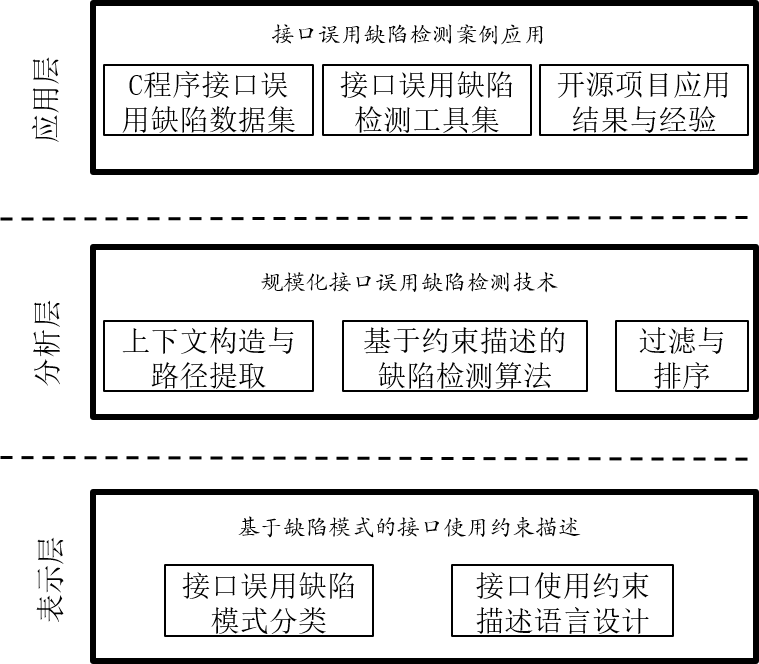
\includegraphics[width=0.85\linewidth]{figures/cp1-overview.png}
	\caption{
		论文研究思路
	}
	\label{fig:1-3-overview}
\end{figure}

随着软件规模增长、代码复杂度提高以及开源代码的广泛使用,现有的API误用检测方法面临巨大挑战。
因此,本文旨在提高接口误用缺陷检测能力,以应对实际项目中接口误用检测精度与规模的矛盾关系。
即在大规模实际项目中支持多种接口误用缺陷类型的同时,尽可能地保证检测的精度。
特别地,C语言多应用于操作系统、嵌入式系统、服务器、数据库等基础软件,需要极高的可靠性和安全性。
因此,本文以C语言作为载体。
针对上述当前研究面临的问题,
本文将提出基于静态分析的C程序接口误用缺陷检测技术
和相关的支持工具集合Tsmart-IMChecker。
整体的研究思路如图~\ref{fig:1-3-overview}所示。
本文将从自底向上的3个层次展开研究:表示层、分析层和应用层。
表示层关注接口使用约束的描述,侧重接口使用约束的描述能力。
对API使用约束条件进行描述是接口缺陷检测的重要基础。
因此,该研究对有效检测接口误用缺陷至关重要。
分析层关注接口误用缺陷检测的方法,侧重检测方法对实际程序中规模与准确性的平衡关系。
随着开源社区的发展,现代软件呈现出大规模、复杂化的特点。
因此,高效、准确的检测方法,是提高代码质量的重要方法。
应用层关注接口误用缺陷检测方法在实际项目中的应用效果,
侧重接口误用测试数据集整理和工具在实际中的应用效果。
本文将总结C程序接口误用缺陷数据集,
开发可视化支撑接口误用缺陷检测工具集。
并将工具在开源项目应用的经验进行总结,
以帮助研究人员和开发人员更好地理解接口误用缺陷。

本文的具体研究思路如下:
\begin{enumerate}
	\item {\kaishu 基于缺陷模式的接口使用约束描述。}
	规约描述语言能够有效地定义API使用的约束条件。
	然而当前已有规约描述语言多关注于接口的实现或特定应用场景。
	自动规约挖掘技术则面临有效数据集缺失的问题,难以支持实际项目中接口误用缺陷的特性。
	因此本文选择接口误用缺陷模式作为切入点,设计一套轻量级的接口使用约束领域特定语言。
	(1)为理解C程序接口误用缺陷的常见模式,本文将对不同领域的开源项目中的实际接口缺陷报告进行调研,
	总结常见接口误用缺陷模式。
	(2)针对C程序接口误用缺陷的常见模式,设计一套面向C程序接口使用约束的领域特定语言。
	该语言应支持多种接口使用约束模式的描述,同时易扩展到新的接口缺陷类型。
	本部分重点研究接口使用约束描述的表达能力,是本文研究的重要基础。
	
	\item {\kaishu 规模化接口误用缺陷检测技术。}
	现代软件具有规模大、结构复杂的特点。
	因此,静态分析的分析效率(大规模程序)与检测准确性(误报率和漏报率)难以同时满足。
	针对两者平衡这一关键问题,面向接口误用缺陷的特点,本文关注如何对静态分析任务进行分而治之,
	以缓解分析过程中路径、状态爆炸等问题。
	同时,在支持大规模代码分析的同时,做到对局部代码的精确分析。
	(1)针对大规模目标程序,本文将采用多入口分析策略,提取和接口缺陷相关的抽象符号路径语义信息,
	并设计基于约束描述的接口缺陷检测算法,以支持用户自定义的接口。
	(2)为降低多入口分析带来的精度损失,本文将通过基于上下文的语义信息和基于使用情况的的统计信息,
	对检测结果进行过滤与排序,以提高检测的精度。
	本部分重点研究检测方法对分析效率和准确性平衡关系,是本文研究的核心技术方法。
	
	\item {\kaishu 接口误用缺陷检测应用。}
	为帮助研究人员更好地理解C程序接口误用缺陷,满足开发者的使用需求,
	本文将提供C程序接口误用缺陷数据集APIMU4C与C程序接口误用缺陷检测工具集Tsmart-IMChecker。
	(1)为帮助研究人员与开发者更好地理解C程序接口误用缺陷,
	本文将对接口误用缺陷模式调研中的实例进行总结。
	同时,为更好地评估现有接口缺陷检测工具的能力与引导新的检测技术的开发,
	本文将结合现有测试数据集与接口误用缺陷模式,构造针对C程序的接口误用测试数据集。
	(2)
	如何降低用户的使用代价和提供有效的缺陷展示功能以辅助开发者理解缺陷是使用者对静态分析工具的迫切需求。
	因此,为提高检测工具的用户友好性以及辅助使用者理解缺陷检测结果,
	本文将开发一系列可视化的工具来辅助开发者进行接口使用约束的撰写、缺陷检测和结果分析。
	(3)
	最后,本文将对工具集在开源项目中进行案例应用,并总结应用的结果和经验。
	本部分重点研究针对C程序接口误用缺陷的数据集以及工具应用,是本文方法的实际应用。
\end{enumerate}




\section{论文贡献}
本文根据上述研究思路,针对C程序接口误用缺陷的静态检测技术进行系统性研究,取得相应的理论效果,
实现了对应的工具软件集合~\cite{19-icse-imchecker, 19-tase-imspec, 19-compsac-empirical}。论文的具体贡献如下:

\begin{enumerate}
	\item 提出用于描述C程序接口使用约束的领域特定语言以及规模化接口误用缺陷检测方法。
	首先,为理解C程序接口误用缺陷的特点,
	本文对不同领域、广泛应用的六个开源项目中830个实际API误用缺陷修复报告进行调研,
	共总结出三大类常见接口误用缺陷模式。
	%据作者所知,这是第一个针对C程序接口误用缺陷的调研工作。
	基于缺陷模式,本文设计C程序接口使用约束的领域特定语言IMSpec,
	并与传统自然语言描述方式对比。
	实验结果表明,IMSpec能够有效描述多种接口使用约束,
	帮助开发者多找到43.7\%的误用缺陷实例。
	同时本文设计并实现基于约束描述的规模化接口误用缺陷检测方法。
	该方法利用多入口分析策略、抽象路径提取和基于程序语义和使用情况的过滤排序技术,
	将规模化代码分析任务分而治之,达到高效率分析的同时,实现局部的精确分析。
	本文选择Juliet Test Suite~\cite{juliet}中13个接口缺陷相关CWE分类的共2172个程序进行评估。
	结果表明,本文提出的方法误报率和漏报率分别为13.21\%和16.80\%,
	优于主流的开源静态分析工具。
	
	\item 总结C程序接口误用缺陷数据集并开发基于图形化的检测工具集。
	基于开源项目和公开测试数据集,本文提供C程序接口误用缺陷数据集APIMU4C。
	据作者所知,这是第一个针对C程序接口误用缺陷的数据集。
	APIMU4C数据集能够帮助研究人员和开发者理解C程序接口缺陷,以及评估检测工具的能力。
	同时本文设计并实现可视化支撑的C程序接口误用缺陷检测工具集。
	在工具集中,本文集成规约撰写工具IMSpec-writer、接口缺陷分析引擎IMChecker-engine
	和基于差异性对比的结果展示工具IMDisplayer,以辅助开发者撰写IMSpec约束文件和理解缺陷检测结果。
	本文将Tsmart-IMChecker工具集应用于广受关注的开源软件中,
	在Linux内核、OpenSSL库以及Ubuntu操作系统中找到超过112个新的接口误用缺陷。
	至今,在75个提交的缺陷报告中,61个缺陷被开发者确认,其中32个已经被开发者在主分支修复。
	本文对实际应用 结果和经验进行总结,供研究人员和开发人员参考。
	
	
	
\end{enumerate}
\section{论文结构}
本文共包括5个章节。第2章介绍针对接口使用约束的领域特定语言,
包括基于实际案例的接口误用缺陷模式以及领域特定语言的设计思路、语法和语义。
第3章讨论规模化接口误用缺陷静态检测方法。
第4章对接口误用缺陷数据集和检测工具集进行介绍,并对工具集在开源项目的应用结果进行总结。
最后第5章总结全文并展望延伸本文工作的若干方向。

\chapter{接口使用约束描述方法研究}
\label{cha:impsec}
随着软件规模的提升与开源社区的蓬勃发展,
开发者经常利用现有的应用编程接口(API)来快速构建系统。
在使用API完成特定功能时,
需要满足对应的约束条件。
例如:检查参数的有效性,正确的调用序列等等。
违反这些约束中的一条或多条,
则会产生接口误用(API misuse),
导致程序错误、系统崩溃,甚至被攻击者利用。
对接口使用约束进行描述,
是避免接口误用的前提条件。
接口行为规约描述语言(BISL)提供面向代码层次的形式化描述,
能够有效的帮助开发者理解API的行为以及使用条件。
因此,基于接口误用缺陷特点的领域特定语言是接口使用约束描述的有效方法。


本章首先针对不同领域的开源C程序中接口误用缺陷实例进行分析,
总结常见缺陷模式。
接着基于缺陷模式,提出C程序接口使用约束领域特定语言IMSpec,
并对语言的设计动机进行介绍,定义该语言语法和语义。
本章将IMSpec应用于调研中收集的接口缺陷实例,以验证语言的有效性。
从全文的研究体系上看,本章的工作旨在通过形式化的方法对接口使用约束描述,
是接口缺陷检测工作的重要基础。


\section{引言}
开发者在使用API构造软件系统时,
需要满足特定的使用约束条件以正确的完成相应的功能。
例如:API参数为指针类型时,该指针不可以为空,
否则可能会产生一个空指针错误;
当通过内存管理接口申请内存资源后,需要使用相应的释放接口以归还资源,
否则产生一个内存泄漏错误。
这些由于误用API产生的缺陷是软件错误、系统崩溃的重要原因之一,
甚至会被攻击者利用,带来巨大影响。


为了保证API的正确使用,
一方面,API的设计者提供了各种各样的文档、应用案例,
以帮助使用者理解API的功能和对应的使用约束条件,
然而,现在的文档形式难以满足实际需求~\cite{09-icse-doc}。
更严重的是,随着开源软件的蓬勃发展,
大量的软件库没有完整的文档资料,
甚至没有或者存在错误的使用说明~\cite{15-ieee-doc-fail, 17-icse-api-doc}。
同时,相对于直接查找官方的API使用文档,
更多的开发者通过网络搜索来快速的找到相应的使用方法。
但是网络资源的可靠性难以保障~\cite{18-icse-stack}。
另一方面,研究人员通过缺陷检测的方法对API误用进行查找,
以提高代码质量。
然而现有的检测方法难以满足实际需求。
基于静态分析技术的检测工具,
多通过预先实现的检测器来进行缺陷查找~\cite{15-coufless-static-survey}。
因此,该方法难以找到为定义的API缺陷。
基于数据挖掘技术的方法,通过推理API使用余数,
再基于这些约束来进行缺陷检测。
然而,现有的数据集质量难以满足学习算法的数据要求~\cite{survey18}。
因此,
无论是API的设计人员还是缺陷检测的研究人员,
如何有效的定义API使用约束是保证接口正确使用的重要基础。

BISL提供面向代码级别的形式化描述方法,
能够有效的帮助程序员理解API的行为以及使用条件~\cite{survey12}。
通俗来说,这些规约描述为接口的开发者和使用者提供一种形式化的契约模式(software contract)~\cite{92-ieee-contract}。
即,这些规约描述通过形式化的表达形式描述
API在使用时需要满足的特定约束条件。
然而,针对于API使用约束的描述,
现有的BISL具有若干不足:
(1)现有的针对普适性程序特征的BISL多面向接口实现而设计,
即有利于描述API的内部属性。
随着软件的规模和复杂性增加,API的使用情景复杂化。
普适性的BISL描述API使用约束条件的易用性不足。
(2)现有的针对接口使用约束的BISL通常为某个特定领域的接口而设计,
语言表达能力不足,难以应用到普适性的API使用约束条件。
例如:SLIC~\cite{01-slic}针对于Windows驱动程序设计,
SSLINT~\cite{15-sp-sslint}针对于SSL的若干API设计。


为解决上述方法中的不足,本章提出IMSpec领域特定语言(DSL),
一个基于缺陷模式的C程序接口使用约束描述语言。
首先,为能够深入理解C程序接口误用缺陷的特点从而总结接口使用约束模式,
本章以不同领域、广泛使用的六个开源软件为对象,
对近五年来830个实际接口误用实例进行分析。
本文共总结出三大类常见接口缺陷模式:
(1)不正确的参数使用(Improper Parameter Using, IPU),
(2)不正确的异常处理(Improper Error Handling, IEH),
(3)不正确的因果调用关系(Improper Causal Calling, ICC)。
这些缺陷模式一方面可以为描述语言的设计提供基础,
简化语言的复杂度。
另一方面,有利于辅助研究人员和开发者理解实际项目中的缺陷模式,
从而提高接口设计以及避免接口误用。
基于缺陷模式,本章提出面向C程序接口使用约束的领域特定语言IMSpec。
本章对IMSpec的设计原则进行介绍,并定义语法结构与形式化语义。
最后,本章将IMSpec应用于调研中发现的典型缺陷实例中,
以展示该语言的描述能力和有效性。
结果显示,IMSpec能够支持调研实例中90.67\%的接口使用约束,平均每个实例4.35行,
对接口使用约束具备描述能力。
同时,在和基于自然语言描述方式的对比中,
实际开发者基于IMSpec多找到了43.7\%的缺陷。
因此IMSpec能够有效地对接口使用约束进行描述。


本章其余部分组织结构如下:
\ref{sec:2.2}节对相关研究进行总结;
\ref{sec:2.3}节给出接口误用缺陷调研的方法,总结调研结果;
\ref{sec:2.4}节给出IMSpec的设计思路,定义语法与语义;
\ref{sec:2.5}节对IMSpec进行实际案例应用与评估;
最后在\ref{sec:2.6}节总结本章工作。

\section{相关工作}
\label{sec:2.2}
本章相关的研究包括两个方面:
接口使用相关的调研工作与规约描述语言的设计工作。
本节将分别对这两方面内容进行总结。

\paragraph{接口使用调研}
过去的二十年内,研究人员对接口使用从不同的角度开展大量的调研工作以保证其被正确使用
~\cite{16-icse-cry,17-tse-survey, 12-fse-parallel,12-fse-deprecation,	18-sqj-evolution,11-etaps-doc, 15-ese-evolution, 11-ese-learning, 15-tse-change,13-etaps-mapping}。
一方面,研究人员从API本身入手,
对API文档~\cite{12-fse-deprecation, 18-sqj-evolution,11-etaps-doc}、
API演化~\cite{15-ese-evolution,15-tse-change}等进行分析;
另一方面,则从使用者的角度,对API使用中的问题进行分析~\cite{16-icse-cry,17-tse-survey,12-fse-parallel,11-ese-learning,13-etaps-mapping}。

随着软件库的更新,新的API用来替换过时的API,
以增加稳定性以及提升效率。
使用这些过期的API,则导致API误用。
Robbes~\cite{12-fse-deprecation, 18-sqj-evolution}在超过2600个系统中分析了577个不同的API,
以分析使用过期API带来的影响。
其结果显示,虽然只有14\%的API在升级后会与其他的系统模块相关,
但是这些改变会带来极大地影响。
其中最多的一个API实例涉及到80个开发者,120个项目。
然而,很多开发者对此并没有做出相应的更新措施,
极大地降低系统的可靠性。

从使用的角度,Zhong~\cite{17-tse-survey}针对于不同类型API的使用情况进行调研分析,
总结出9个与API使用相关的发现,
以设计更好的规约挖掘技术。
特别地,该论文指出,在对API使用进行规约描述时,
需要考虑非顺序调用关系、类型信息和顺序关系三个特点。
同时,随着多核处理器的发展,开发人可以利用并行化技术来加快问题求解。

Okur~\cite{12-fse-parallel}对655个开源项目中并行计算软件库中的API使用情况进行分析。
结果显示,超过10\%的开发者误用这些API,导致程序并没有并行化运行,而是在串行执行。
同时,由于对API使用规则的生疏,开发者撰写的代码复杂度高,难以理解与维护。

与Okur的工作类似,Nadi~\cite{16-icse-cry}针对加密算法的API使用情况进行分析。
该研究针对100个StackOverflow的问题与回答、100个Github上的开源项目和48个实际开发者进行调研。
其结果显示,尽管开发者认为这些API使用难度大,但是他们依旧坚信能够正确使用这些接口。
但是,加密算法相关API误用却普遍存在~\cite{13-ccs-misuse}。

Robillard~\cite{11-ese-learning}从开发者的角度对API使用进行调研。
通过多阶段的调研问卷与面对面的讨论,
该研究发现开发者认为API学习难度大。
其主要原因是现有的文档形式难以有效地帮助使用者理解如何正确使用接口。
特别地,缺少足够的使用样例是文档最大的不足。
因此,虽然API的设计者提供了格式良好的文档,
但是开发者多利用网络资源以快速的掌握API的使用情况。
%这也对缺陷检测后的结果展示提出要求。

现有的接口使用调研工作多针对面向对象编程语言展开~\cite{16-icse-cry,17-tse-survey, 12-fse-parallel,12-fse-deprecation},
因此其结果难以直接应用于C程序。
针对接口误用缺陷,Okur对并行化API的缺陷模式进行分析以及
Nadi对加密算法相关的API使用情况进行分析。
这些方法都只针对于某一个特殊领域,其结果难以直接适用于普适性接口缺陷模式。


\paragraph{规约描述语言}
软件行为规约(behavorial specification)是对软件系统或者组件预期行为的精确描述。
独立的代码实现并不能有效描述其功能和使用约束,
所以规范记录下来的信息对于软件维护有着重要的作用,
能够有效的描述API开发者和使用者之间的协议~\cite{92-ieee-contract}。
特别地,形式化的规约描述语言能够消除自然语言的歧义。
规约能够在软件的整个开发周期使用。
一方面,开发人员可以根据规约进行内部功能实现。
另一方面,测试人员能够在调试阶段根据规约去分离错误,划分责任~\cite{05-vstte-spec}。
近三十年来,研究人员针对不同的语言和目标,设计并实现各种各样的BISL~\cite{survey12}。
例如,针对通用属性检测的BLAST~\cite{blast}、ACSL~\cite{acsl};
针对领域特定的BISL,包括:SSL安全的SSLINT~\cite{15-sp-sslint}、
Windows内核驱动程序的SLIC~\cite{01-slic}、Epex工具中对异常处理检测的规约~\cite{16-sec-epex}等等。


BLAST~\cite{blast}由Dirk Beyer教授提出,是面向时序安全属性的规约描述语言,
用于BLAST自动化验证工具。
该语言从两个不同的精度水平对程序属性进行描述。
微观来说,该语言能够通过描述检测自动机(monitor automata)的内部转移,
以在程序的运行时轨迹上对程序时序属性进行分析。
宏观来讲,该语言通过撰写可达性查询语句,
对程序的状态与位置进行查询。
通过两个精度水平的描述,能够有效的将验证问题转化到多个独立的模型检测引擎中,
以降低验证工作的复杂性。

ACSL(ANSI/ISO C Specification Language)是Frama-C~\cite{16-rv-framac}代码分析平台用来形式化定义C程序属性的规约描述语言。
该语言通过注释的方式对程序中属性进行描述,以辅助验证工具对代码实现情况进行检测。
ACSL注重函数合约(function contract),
即函数的参数与函数执行后需要满足的性质。
其中,前者也被称作前置条件(pre-condition);后者被称作后置条件(post-condition)。
特别地,前置条件多针对于API使用者,即在调用目标API之前需要满足的约束。
ACSL以代码注释的形式撰写,因此,为了利用ACSL,
分析工具需要理解ACSL的语法与语义,同时将ACSL与目标C程序的源代码进行转化。


针对于C程序接口误用缺陷检测,微软公司SLAM项目~\cite{slam}是典型代表之一。
开发者通过使用SLIC规约描述语言~\cite{01-slic}对程序接口的属性进行描述,
并使用基于反例引导的抽象解释技术的SDV验证工具对目标API进行检查。
至2010年,该项目已经积累超过200个API使用规约,
成功检测到Windows操作系统驱动程序中270个API误用缺陷,
有效提高接口使用的正确性~\cite{10-cad-slam, 11-acm-slam}。
此外,SSLINT基于程序依赖图(program dependency graph)对SSL安全相关的API进行建模,
并通过Cypher~\cite{18-sigmod-cypher}图查询语言对预定义好的模式进行查询,
以检测API误用。
Epex对API返回值的约束条件进行描述,
并利用规约对C程序中接口误用后异常处理缺陷进行检测。

现有规约描述语言对于C程序接口使用约束的描述存在若干不足。
一方面,通用语言针对多种程序属性设计,多针对于功能实现设计,语法结构多样,语义丰富。
然而,接口使用多含有复杂的程序结构,设计多个API的协同使用。
因此通用语言描述使用约束需要复杂的组合。
另一方面,现有针对接口使用的描述语言多针对某个特定领域或者某个特定接口使用类型,
难以扩展到普适性的接口使用约束。
例如SLIC语言能够有效的应用于Windows操作系统驱动程序,
却难以应用于SSL安全库中的接口。


\section{接口误用缺陷分类}
\label{sec:2.3}
为能够在实践中更加有效的解决API误用问题,
对API误用缺陷的特点进行深入研究以总结API误用缺陷类型具有重要意义。
一方面,可以通过缺陷分类标准进行提取;
另一方面则可以通过现有研究中接口误用缺陷对象进行概括与总结。

IEEE组织在1993发布IEEE-1044软件异常分类,并在2009年更新~\cite{09-ieee-classification}。
基于该标准的内容,IBM公司提出Orthogonal Defect Classification(ODC)分类标准~\cite{92-tse-odc}。
ODC基于缺陷类型(defect type)对缺陷进行分类,
即通过代码结构的组成进行分类。
例如函数、检测、赋值、文档等等。
%一个缺陷类型具体可以表现为两种异常类型(violation type),即缺失或者误用。
2016年Beller~\cite{16-saner-evaluation}基于ODC提出General Defect Classification(GCD),
以更加精确的比较静态分析技术的检测能力。
然而现有的缺陷分类方式,一方面没有对所有的软件缺陷进行描述,因此无法涵盖所有接口误用缺陷域;
另一方面缺少对API误用缺陷的详细分类情况。

过去的十几年内,研究人员对不同的接口误用缺陷进行过检测。
例如,Monperrus~\cite{13-tosem-missing-call}研究指出,
缺失必要的API调用普遍存在于缺陷跟踪系统、论文和源代码以及代码的注释中。
Thummalapenta~\cite{09-icse-exception}针对API调用前需要满足的前置条件进行研究。
Wasylkowski~\cite{07-fse-object}则对接口调用的顺序错误进行检测。
然而,这些研究都只针对接口缺陷中某一个特定的种类。
Adama~\cite{survey18}在其研究结果中,针对Java程序提出API-Misuse Classification(MUC),
以对API误用缺陷进行分类,并比较现有工具的检测能力。
该分类基于API使用元素与缺陷表现类型进行分类。
一个缺陷类型具体可以表现为两种异常类型(violation type),即缺失(missing)或者误用(misuse)。
本文针对C程序的API缺陷进行研究,C程序与Java程序存在巨大设计理念差异。
该结果难以直接应用于本文研究内,但是对本文的研究就有重要参考意义。
另一方面,研究人员从API使用本身入手,
调研并给出针对于API使用说明性质的(directive)分类~\cite{09-icse-doc,12-ese-directive}。
API使用说明,是API文档中的一段自然语言描述,
用来提醒开发者在使用API时需要满足的约束条件。
当这些约束条件被使用者忽略或者违反时,认为使用者产生了一个API误用。
然而只有部分说明可以直接对应于误用以及产生的缺陷,其他的则更注重API的内部功能或者特殊用法。
例如:明确地说明API的参数可以为空是针对API使用中不同方式的引导。
不过这些调研结果可以作为本文的重要参考内容。


据本文作者调研结果显示,目前并没有工作对C程序接口误用缺陷的问题域进行定义或描述。
因此,研究人员难以对直接对现有研究进行系统的了解与总结。
特别是哪些API缺陷种类已经被研究过和哪些没有被研究过,
以及现有的方法能够解决多少问题和方法之间的效果比较。
因此,为更好的应对C程序API误用缺陷检测,
我们需要一个具有针对性以及来源于实际程序的缺陷类别,帮助设计更有效的接口使用约束描述方法。
本节剩余部分将对数据收集和分类结果进行详细描述,
并对接口缺陷分类调研结果进行讨论。

\subsection{数据收集}
本小结将针对数据收集的主要步骤进行详细描述,
包括研究对象、缺陷实例收集方法和缺陷分析方法。

\paragraph{研究对象}
\begin{table}[t]
	\centering
	\begin{minipage}[t]{0.9\linewidth} % 如果想在表格中使用脚注,minipage是个不错的办法
		\caption{API误用缺陷研究对象。}
		\label{tab:2-3-target}
		\begin{tabular}{lp{3cm}<{\centering}p{3cm}<{\centering}p{4cm}<{\centering}}
			\hline
			{\heiti 研究对象} & 
			\multicolumn{1}{c}{\heiti 关注数\footnote{本文选取Github上Watch和Star中较多者。}} &
			\multicolumn{1}{c}{\heiti 提交次数} & 
			\multicolumn{1}{c}{\heiti 可用时间\footnote{Github上可以追溯的代码修改时间。}} \\
			\hline
			Linux内核   & 69,697 & 812,391 & 20050416-至今\\
			OpenSSL   & 9,510 & 23,412 & 19981221-至今\\
			FFmpeg   & 13,907 & 93,218 & 20001220-至今\\
			Curl   & 24,009 & 12,130 & 19991229-至今\\
			FreeRDP   & 2,959 & 13,030 & 20110630-至今\\
			Httpd   & 2,028 & 31,341 & 19960703-至今\\
			\hline
		\end{tabular}
	\end{minipage}
\end{table}


当代软件开发模式多利用开源社区已有的实现,对功能进行封装,
因此对开源软件的研究更加迫切。
为能够更好地理解现实中C程序API误用缺陷的特点以及开发者如何对这些缺陷进行修复,
本文对不同领域、广泛使用的六个开源软件进行分析。
如表\ref{tab:2-3-target}所示:
这六个项目为:
\begin{enumerate}
	\item Linux内核~\cite{linux}:
	Linux内核是一种开源的类Unix操作系统内核,由芬兰赫尔辛基大学学生Linus Torvalds于1991年创建。
	该内核由一系列的程序组成,包括中断服务程序、负责管理多个进程从而分享处理器时间的调度程序、
	负责管理地址空间的内存管理程序、网络、进程间通信的系统服务程序等。
	随着开源社区的发展、软件日益复杂的功能和各种硬件的发展,越来越多的驱动程序被集成在Linux内核中。
	Linux内核在近年来发展迅速,代码量已经到达13000kLOC。
	
	\item OpenSSL~\cite{openssl}:
	安全套接层协议(SSL)可以在网络上对传输内容进行加密,以提供秘密性传输的功能。
	OpenSSL则是实现该协议的开源软件库。
	该库提供三个主要的功能模块:SSL协议库、密码算法库以及应用程序。
	OpenSSL提供强大和全面的功能,囊括主要的密码算法、常用的密钥和证书封装管理功能以及SSL协议,
	并提供丰富的应用程序供测试或其它目的使用。
	应用程序可以使用OpenSSL进行安全通信,避免窃听。
	
	
	\item FFmpeg~\cite{ffmpeg}:
	FFmpeg是一套针对多媒体处理的开源软件库与应用程序,
	可以用来记录和转换数字音频、视频,
	并能将其转化为流数据。
	该库由若干子项目组成,包括:多媒体编码解码算法、
	公用工具函数库、视频场景处理库、
	后期效果处理库、格式转换、基于HTTP多媒体及时广播串流服务器以及
	多媒体播放器等等。
	
	\item Curl~\cite{curl}:
	Curl是一个利用URL语法~\cite{url},在命令行下工作的文件传输工具。
	该工具支持文件的上传和下载,被称作为综合传输工具。
	Curl支持多种通信协议,同时还提供多种安全验证机制。
	自1997年首次发行以来,该工具被开发者广泛应用,吸引上千开发者的贡献。
	已经成功应用于汽车、电视、交换机、打印机、手机、平板电脑等多个领域。
	同时,Curl还提供基于程序开发的libcurl接口库。
	
	\item FreeRDP~\cite{freerdp}:
	远程桌面协议(Remote Desktop Protocol,RDP)是一个多通道的远程连接协议,
	能够让客户端连接提供远程服务的Windows服务机。
	FreeRDP是一款基于Apache协议实现RDP协议的开源软件。
	目前该软件已经成功应用于多个Linux发布版以及Mac系统。
	
	
	\item Httpd~\cite{httpd}:
	Httpd是Apache开源组织研发面向超文本传输协议(HTTP)服务器的主程序。
	该程序以独立运行的后台进程存在,并通过子进程或者线程池形式对请求进行处理。
	Httpd代码开源,并被广泛应用于各种网络服务中,
	目前已经成为网络上最受欢迎的服务器之一。
	
\end{enumerate}

上述研究对象涵盖不同的领域:操作系统(Linux内核),开源API库(OpenSSL和FFmpeg),
Ubuntu应用软件(Curl,FreeRDP和Httpd)。
具有多年的开发历史,并且现在依旧活跃于开源社区中,
被应用人员广泛使用。
一方面,活跃的开发者和用户社区有利于缺陷的报告和修复;
另一方面,被广泛使用使得这些软件的代码质量更具有代表性。
特别是针对于代码质量,
大量的使用者和开源社区贡献,能够快速的对程序中的缺陷进行修复。
同时,这些项目都在Github网站上开源、具有完整的修改记录和缺陷跟踪系统。
这些修改记录和缺陷跟踪系统有利于对缺陷实例的收集和总结。
因此,本文对以上项目进行分析。
本文将数据抽取的工具和方法公布,
方便研究人员和开发者进行扩展或者研究其他领域问题。

\paragraph{缺陷实例收集}
\begin{table}[t]
	\centering
	\begin{minipage}[t]{0.9\linewidth} % 如果想在表格中使用脚注,minipage是个不错的办法
		\caption{API误用缺陷研究对象}
		\label{tab:2-3-statistics}
			\begin{tabular}{crcrrr}
			\hline
			\multirow{2}{*}{项目名称} & \multirow{2}{*}{Loc} & 研究 & \multicolumn{1}{c}{修改}& \multicolumn{1}{c}{缺陷}& \multicolumn{1}{c}{API误用}\\
			&  & 时间 & \multicolumn{1}{c}{总数} & \multicolumn{1}{c}{数目}& \multicolumn{1}{c}{数目} \\
			\hline
			Linux & 12.96M & 20170901-20171231 & 24651 & 6401 & 868 \\
			%\hline
			OpenSSL & 454K & 20150701-20171231 & 7564 & 2391 & 529 \\
			%\hline
			FFmpeg & 915K & 20160701-20171231 & 8162 & 2783 & 610 \\
			%\hline
			Curl & 113K & 20130101-20170630 & 7082 & 2043 & 499 \\
			%\hline
			FreeRDP & 259K & 20130701-20171231 & 7565 & 3535 & 495 \\
			%\hline
			Httpd & 203K & 20130701-20171231 & 6072 & 1323 & 149 \\
			\hline
			Total & 14.90M & - & 61096& 18476 & 3150 \\
			\hline
		\end{tabular}
	\end{minipage}
\end{table}


本文通过对软件开发的版本修改记录日志分析,以完成API误用缺陷实例收集工作。
如表\ref{tab:2-3-statistics}所示,本文在六个开源项目中,
共对61096个修改记录进行分析,在18476个缺陷修复记录中收集3150个API误用缺陷实例。
下文将详细描述缺陷实例的收集方法。

首先,通过Github上的日志记录追踪系统,对所有的修改记录进行下载和备份。
针对于每一次修改记录,抽取修改说明(description)、
修改的差异性报告(diff文件)以及修改前和修改后的源代码文件。
图\ref{fig:2-3-description}给出Linux内核修改sha:059c98599的修改说明。
包括:修改的哈希值、概要总结、详细说明、作者、时间以及上一版本的哈希值。
根据本次修改的哈希值以及上一修改的哈希值,可以抽取(checkout)相应版本的源文件,
即修改前和修改后的文件。
图\ref{fig:2-3-diff}给出该修改的差异性报告。
其中以“+”开始的绿色行为增加的行,以“-”开始的红色的为删掉的行。

\begin{figure}[t]
	\centering
	\begin{minipage}{0.75\linewidth}
{\footnotesize	
%\begin{lstlisting}
"hash": "059c98599b1ab1e2e479e1f4617948d4c2a32b84",\\
"summary": "wl18xx: add checks on wl18xx\_top\_reg\_write() return value",\\
"description": 
"wl18xx: add checks on wl18xx\_top\_reg\_write() return value.
Check return value from call to wl18xx\_top\_reg\_write(),
so in case of error jump to goto label out and return.
Also, remove unnecessary value check before goto label out.\\
Addresses-Coverity-ID: 1226938\\
Signed-off-by: Gustavo A. R. Silva <garsilva@embeddedor.com>\\
Signed-off-by: Kalle Valo <kvalo@codeaurora.org>",\\
"date": "2017-06-28 21:18:40",\\
"author": "Gustavo A. R. Silva",\\
"parent\_hash": "69551f5f370cc20342fab17ca54716b6ec7e332d"	
%\end{lstlisting}
}
	\end{minipage}
	\caption{
	Linux内核修改sha:059c98599的修改说明。
	}
	\label{fig:2-3-description}
\end{figure}
\begin{figure}
	\centering
\begin{lstlisting}
drivers/net/wireless/ti/wl18xx/main.c
=======================================================
lhs: 100644 | d1aa3eee0e81f8cc7612eddabc4cf630dbbd1e79
rhs: 100644 | 0cf3b4013dd646104b1f153c3d8a191f12a5dba8
@@ -793,9 +793,13 @@ static int wl18xx_set_clk(struct wl1271 *wl)
ret = wl18xx_top_reg_write(wl, PLLSH_WCS_PLL_P_FACTOR_CFG_2,
	(wl18xx_clk_table[clk_freq].p >> 16) &
	PLLSH_WCS_PLL_P_FACTOR_CFG_2_MASK);
+		if (ret < 0)
+			goto out;
} else {
ret = wl18xx_top_reg_write(wl, PLLSH_WCS_PLL_SWALLOW_EN,
	PLLSH_WCS_PLL_SWALLOW_EN_VAL2);
+		if (ret < 0)
+			goto out;
}

/* choose WCS PLL */
@@ -819,8 +823,6 @@ static int wl18xx_set_clk(struct wl1271 *wl)
/* reset the swallowing logic */
ret = wl18xx_top_reg_write(wl, PLLSH_COEX_PLL_SWALLOW_EN,
	PLLSH_COEX_PLL_SWALLOW_EN_VAL2);
-	if (ret < 0)
-		goto out;

out:
return ret;

\end{lstlisting}
	\caption{
	Linux内核修改sha:059c98599的差异性报告。
	}
	\label{fig:2-3-diff}
\end{figure}

接着对修改记录进行分析,抽取本文关心的接口误用缺陷实例。
如表\ref{tab:2-3-statistics}所示,在六个项目中,本文共抽取61096个修改记录实例。
由于不同的领域背景、代码的复杂性、接口的熟悉程度等原因,
在现阶段情况下,针对每一个实例进行分析难以完成。
因此本文通过自然语言处理的方式,在修改说明中对接口误用缺陷进行抽取:
\begin{enumerate}
	\item 针对六个项目,本文随机的在每一个项目中选择100个修改记录实例进行详细分析。
	通过API文档研究、代码查看、开发者讨论等方式,本文筛选出与缺陷修复(bug fix)相关的实例,
	并总结这些实例中的普适性关键词。
	例如:“bug”,“error”,“fix”和“check”等等。
	\item 在缺陷修复相关的实例中,进一步筛选和API误用缺陷相关的实例。
	本文利用在已发表论文中的缺陷类型以及其他针对软件缺陷分类中的类型作为基础,
	对缺陷的原因进行判断。
	如果缺陷的产生原因出现在上述分类中的一种或者多种,那么就认为这是一个API误用缺陷。
	本文对这些缺陷修改中描述的普适性关键词进行总结,
	例如:“fix API”,“missing check”,“null pointer dereference”,“add check” “memory leak”以及“return value”等等。
	\item 基于这些关键词本文在已经抽取的所有缺陷实例中进行文本匹配,
	通过筛选缺陷修改说明来获取目标研究对象中的缺陷实例。
	对于选中的结果,本文过滤掉所有没有修改过*.c源文件的修改记录。
\end{enumerate}

图\ref{fig:2-3-description}和图\ref{fig:2-3-diff}是一个缺陷实例。
在Linux项目中,通过关键词的所搜,本文认为修改sha:059c98599的修改与缺陷修复有关。
因为修改的描述中包含关键词“check”,即“\underline{Check} return value from call to wl18xx\_top\_reg\_write()”。
此后在API误用缺陷搜索的过程中,
该修改还包括“\underline{add checks} on wl18xx\_top\_reg\_write() return value”。
因此,本文认为该修改与接口缺陷相关。
如图\ref{fig:2-3-diff}所示,该修改用来修复不正确的API返回值检查缺陷。
该缺陷的原因以及缺陷模式将在后文中进行详细分析。

针对于该方法的有效性,本文在抽取的结果中通过随机取样进行验证。
在所有的API误用缺陷修复实例中,本文在每个项目中随机抽取了30个样例。
通过对这180个实例的详细分析,发现其中的166个是API误用缺陷修复实例,
即准确率达到92.22\%。
在所有的误报实例中,虽然修改说明中出现相应的关键词,
但是修改的内容本身与API误用无关。
例如:OpenSSL的一个修改记录sha:4af389为“Fix compilation with OPENSSL API compat”。
该描述中包含“fix API”关键词,然而,该修改针对于编译错误。
因此,本文认为通过以上方法能够有效的在修改记录中获取API误用缺陷实例。

在预实验阶段,由于缺少领域知识、对API掌握熟练度不足、以及缺陷的复杂性,
平均每个缺陷的理解时间在3.5小时。
特别地,有的缺陷报告涉及多个文件,包含API缺陷修改、重构、文档等多个内容。
现阶段情况下难以在有限的时间内,针对每一个实例进行详细分析。
因此,本文在3150个API误用缺陷实例中,
在每个项目中抽取35\%的缺陷实例。
针对于这部分缺陷,进一步将修改超过两个文件、修改行数大于30行的修改记录进行过滤。
如表\ref{tab:2-3-studied}所示,最终本文在3150个API缺陷实例中,
对随机抽取的830个缺陷实例(26.35~\%)进行深入分析。

\begin{table}[t]
	\centering
	\begin{minipage}[t]{0.85\linewidth} % 如果想在表格中使用脚注,minipage是个不错的办法
		\caption{API误用缺陷实例统计信息}
		\label{tab:2-3-studied}
		\begin{tabular}{cccccc}
			\hline
			\multirow{2}{*}{项目名称} & \multirow{2}{*}{缺陷总数} & \multicolumn{2}{c}{API误用}& \multicolumn{2}{c}{研究实例}\\
			\cline{3-4}\cline{5-6}
			&  & 数量 & 百分比(\%)\footnote{与缺陷总数的百分比} & 数量& 百分比(\%)\footnote{与API误用缺陷总数的百分比} \\
			\hline
			Linux & 6401 & 868 & 13.56 & 283 & 32.60 \\
			%\hline
			OpenSSL & 2391 & 529 & 22.12 &127  & 24.00 \\
			%\hline
			FFmpeg & 2783 & 610 & 21.92 & 126 & 20.66 \\
			%\hline
			Curl & 2043 & 499 & 24.42 & 134 & 26.85 \\
			%\hline
			FreeRDP & 3535 & 495 & 14.00 & 119 & 24.04 \\
			%\hline
			Httpd & 1323 & 149 & 11.26 & 41 & 27.52 \\
			\hline
			总计 & 18476 & 3150 & 17.05 & 830 & 26.35 \\
			\hline
		\end{tabular}
	\end{minipage}
\end{table}
\paragraph{缺陷分析}
基于上述步骤收集的的缺陷实例,本文通过对修改说明文件的内容、差异性报告以及
源代码文件对缺陷进行理解。
包括:接口误用上下文语义中的根本原因、修复的模式以及误用的其他统计信息等。
特别地,为了能够理解API误用缺陷的本质,
本文关注API误用的根本原因,即在API使用的整个代码片段中,哪一部分的错误导致API误用。

以图\ref{fig:2-3-diff}为例。
通过缺陷描述可知,
该缺陷的产生的原因是没有对接口~\texttt{wl18xx\_top\_reg\_write()}的返回值进行检查。
同时,差异性报告中显示,该缺陷的修改方式是增加返回值\texttt{ret}的检查,
即该返回值是否小于零。
此外本文发现,如果小于零则添加\texttt{goto}语句,跳转并进行异常处理。
总结来说,该缺陷产生的上下文是~\texttt{wl18xx\_top\_reg\_write()}函数调用后,没有进行返回值检查;
缺陷的根本原因则是没有对该函数进行异常处理;
修复的模式则相对简单,即进行检查并添加跳转语句。


\subsection{调研结果}
如表\ref{tab:2-3-studied}所示,
在18476个缺陷修复实例中,有3150个与API修复有关,
平均百分比为17.05\%。
其中Curl占比例最多,为24.42\%;
Httpd最少,为11.26\%。
在上文介绍的预实验方法和结果中,平均92.22\%的API误用缺陷为真正例(True Positive,TP)。
因此,本文相信API误用缺陷并不是开发阶段发生的偶然事件。
其具有普遍性。

\vspace*{10pt}
\begin{center}
\noindent\shadowbox{
	\centering
	\begin{minipage}{0.85\textwidth}
		{\kaishu 发现1:API误用缺陷普遍存在被分析系统中。
			调研结果显示,平均17.05\%缺陷修复相关的修改记录与API误用相关。}
	\end{minipage}
}
\end{center}

为能够理解API误用缺陷的本质原因,本文对随机选取的830缺陷实例进行分析,
包括出错的根本原因、误用缺陷的修复模式以及API误用重复发生的统计信息。
下文将对调研的结果进行仔细分析。

\begin{table}[b]
	\centering
	\begin{minipage}[t]{\linewidth} % 如果想在表格中使用脚注,minipage是个不错的办法
		\caption{API误用缺陷实例统计信息}
		\label{tab:2-3-root-causes}
		\begin{tabular}{cccccccccc}
			\hline
			\multirow{2}{*}{项目名称} & 实例 & \multicolumn{2}{c}{IPU}& \multicolumn{2}{c}{IEH}& \multicolumn{2}{c}{ICC}& \multicolumn{2}{c}{其他}\\
			\cline{3-10}
			& 个数 & 数量 & 百分比 & 数量& 百分比 & 数量& 百分比& 数量& 百分比 \\
			\hline
			Linux  & 283 & 43 & 15.1 & {96} & {33.92} & 77 & 27.21 & 67 & 23.67 \\
			%\hline
			OpenSSL  & 127 & 21 & 16.54 & 42 & 33.07 & {49} & {38.58} & 15 & 11.81 \\ 
			%\hline
			FFmpeg  & 126  &  18 & 14.29 & 43 & 34.13 & 52 & 41.27 & 13 & 10.32 \\
			%\hline
			Curl  & 134   & 23 & 17.16 & 38 & 28.36 & 57 & 42.54 & 16 & 11.94 \\ 
			%\hline
			FreeRDP   & 119 & 22 & 18.49 & 30 & 25.21 & 48 & 40.34 & 19 & 15.97 \\ 
			%\hline
			Httpd  & 41 & 8 & 19.51 & 8 & 19.51 & 16 & 39.02 & 9 & 21.95 \\ 
			\hline
			Total  & 830 & \multicolumn{2}{c}{135 (16.27\%)} & \multicolumn{2}{c}{257 (30.96\%)} & \multicolumn{2}{c}{299 (36.02\%)} & \multicolumn{2}{c}{139 (16.75\%)}\\ 
			\hline
		\end{tabular}
	\end{minipage}
\end{table}
\paragraph{根本原因}

在对所有的目标用例分析后,本文将统计结果总结于表\ref{tab:2-3-root-causes}中。
虽然每个项目中,出错的根本原因分布不同。
但是可以总结出三大类常见C程序接口误用缺陷模式:
不正确的参数使用(Improper Parameter Using, IPU)、
不正确的异常处理(Improper Error Handling, IEH)、
不正确的因果调用关系(Improper Causal Calling, ICC)。
下文中将通过缺陷实例对这些缺陷类型进行讲解。

\begin{figure}[b]
	\centering
\begin{lstlisting}
"description": "Fixed API nonnull warning."
"date": "2014-11-17 00:00:09"
"author": "Armin Novak"
libfreerdp/core/gateway/http.c
=======================================================
lhs: 100644 | 4cef378c8cafdc4ad4a237f88a092c511c250ffa
rhs: 100644 | 51c5c04dc257975756a4ee3ded16cae493dea95c
@@ -330,10 +330,12 @@ void http_request_free(HttpRequest* http_request)

BOOL http_response_parse_header_status_line(HttpResponse* http_response, char* status_line)
{
-	char* separator;
+	char* separator = NULL;
char* status_code;
char* reason_phrase;
-	separator = strchr(status_line, ' ');
+
+	if (status_line)
+		separator = strchr(status_line, ' ');

if (!separator)
	return FALSE;
@@ -433,7 +435,10 @@ BOOL http_response_parse_header(HttpResponse* http_response)
*                 |     |
*         colon_pos     value
*/
-		colon_pos = strchr(line, ':');
+		if (line)
+			colon_pos = strchr(line, ':');
+		else
+			colon_pos = NULL;

if ((colon_pos == NULL) || (colon_pos == line))
	return FALSE;

\end{lstlisting}
	\caption{
	FreeRDP中空指针引用导致的IPU-API误用缺陷(sha:9e5be6f7e8)。
	}
	\label{fig:2-3-ipu-1}
\end{figure}

\noindent{\textbf{IPU}}:软件库的开发者提供API,
以实现对特定功能封装,达到软件复用的作用。
然而,开发者在使用这些API的时候,需要满足特定的条件,
以保证API使用时上下文环境正确。
这些API使用前需要满足的条件,亦被称作前置条件(pre-condition)~\cite{14-fse-pre}。

例如,一个API的参数中包含指针类型,
那么通常情况下在调用该API之前,需求保证该指针不为空指针NULL。
然而,本文发现API的使用者经常忽略这些约束条件,
导致空指针解引用错误。
图\ref{fig:2-3-ipu-1}给出一个FreeRDP项目中的缺陷修改记录。
接口\texttt{strchr(str, c)}用来搜索字符串\texttt{str}中,
第一次出现字母\texttt{c}的位置。
其中\texttt{str}是一个指向字符串的指针。
在FreeRDP项目http.c文件中定义的接口\texttt{http\_response\_parse\_header\_status\_line()}中,
将来自外部输入的参数\texttt{status\_line}作为参数传递给\texttt{strchr}。
然而在调用\texttt{strchr}之前(16行与27行),并没有对该参数进行非空指针检查。
如果该参数为空指针,则会产生一个API误用,导致程序崩溃。
为避免该缺陷,开发者增加参数非空检查的条件判断,如图中18-19行与28-31行所示。


\begin{figure}[t]
	\centering
\begin{lstlisting}
"hash": "f7d183f08472e566a2e6b62a80e200a12670ed0e",
(*@\textcolor{black}{"summary": "libxvid: Check return value of write() call",}@*)
"date": "2016-11-11 10:17:07",
"author": "Diego Biurrun",
libavcodec/libxvid_rc.c
=======================================================
lhs: 100644 | eddbbe8c651407bdc85652191a7ba964c1776f74
rhs: 100644 | 94301a2ac1ffc10a8b22ba491c70013463107452
@@ -87,7 +87,10 @@ av_cold int ff_xvid_rate_control_init(MpegEncContext *s)
(rce->i_tex_bits + rce->p_tex_bits + rce->misc_bits + 7) / 8,
(rce->header_bits + rce->mv_bits + 7) / 8);

-    write(fd, tmp, strlen(tmp));
+    if (strlen(tmp) > write(fd, tmp, strlen(tmp))) {
+        av_log(s, AV_LOG_ERROR, "Cannot write to temporary pass2 file.\n");
+        return AVERROR(EIO);
+    }
}

close(fd);

\end{lstlisting}
	\caption{
	FFmpeg中参数、返回值关系的IPU-API误用缺陷(sha:f7d183f084)
	}
	\label{fig:2-3-ipu-2}
\end{figure}
此外,函数参数的关系、参数与返回值的关系也需要考虑。
最典型的就是C标准库中内存操作相关的接口。
例如,接口\texttt{memcpy(d, s, n)}用来从源头内存区间\texttt{s}中,
拷贝\texttt{n}个字符到目标内存区间\texttt{d}。
因此,该函数在使用的时候,目标内存区间\texttt{d}的大小要大于或者等于拷贝长度\texttt{n}。
否则将产生一个内存越界错误。
另一方面,参数与返回值之间也可能存在语义关联关系。
例如,接口\texttt{size t write(int fd, void* buf, size t cnt)}从参数\texttt{buf}指向的内存区域内,
读取\text{cnt}个字符到参数\texttt{fd}所标志的文件或者网络链接(socket)。
该接口的返回值记录实际输出字节个数。
特别地,\texttt{write()}的返回值为负数时,则表明该函数调用发生错误。
因此如果需要确保\texttt{cnt}个字节被写入到目标地址时,
需要检查该值与函数的返回值之间的关系,以保证软件的鲁棒性。
然而如图\ref{fig:2-3-ipu-2}中13行所示,
FFmpeg项目中libxvid\_rc.c文件在调用该接口后并有对返回值与参数进行比对,
从而忽略API参数与返回值之间的约束关系。
为避免该错误,开发者增加返回值与参数之间的约束关系检查,如图中14-17行所示。

\vspace*{10pt}
\begin{center}
	\noindent\shadowbox{
		\centering
		\begin{minipage}{0.85\textwidth}
			{\kaishu 发现2:在所有被研究的API误用缺陷实例中,14.29-19.51\%缺陷产生的原因是
				不正确的参数使用(Improper Parameter Using,IPU),
				包括缺失或者错误地对单个参数属性、参数之间以及参数和返回值之间的约束检查。
			}
		\end{minipage}
	}
\end{center}


\noindent{\textbf{IEH}}:
安全可靠的软件需要对所有可能出错的条件进行捕获,
并对捕获的异常进行对应的处理。
因此,现在编程语言多提供一套完整的异常处理机制,
以保证即使底层的功能出错,系统整体也能够正常处理,不会崩溃。
不幸的是,C语言并没有提供原生的异常处理机制。
所以,在C程序中开发者需要自己定义这样的异常处理机制。
由于缺少统一的处理方式,异常处理代码经常和项目的领域特定信息相关,
形式多样、重复性高、代码繁琐等等。
特别地,当函数调用发生错误后,未能正确进行异常处理则会产生异常处理缺陷,
甚至会导致严重的安全漏洞,
例如:CVE-2014-0092~\cite{CVE-2014-0092},CVE-2015-0208~\cite{CVE-2015-0208},
CVE-2015-0285~\cite{CVE-2015-0285},CVE-2017-3318~\cite{CVE-2017-3318},
CVE-2017-5350~\cite{CVE-2017-5350}等等。
事实上,根据开源网络应用安全项目(The Open Web Application Security Project)指出,
不正确的异常处理是导致软件安全漏洞的十大因素之一~\cite{07-owasp}。

\begin{figure}[t]
	\centering
\begin{lstlisting}
"hash": "086ad79970f3cd0463558bfb69122f6acdc9d2da",
"summary": "ldap: check Curl_client_write() (*@\textcolor{black}{return}@*) codes",
"date": "2014-12-10 00:41:32",
"author": "Daniel Stenberg",
ib/ldap.c
=======================================================
lhs: 100644 | 14437c3b54715cb5ad161d78ee7b89a412b64a9d
rhs: 100644 | 96521bf21862540e32368e229365ed49d6f43cff
---@@ -384,9 +384,17 @@ static CURLcode Curl_ldap(struct connectdata *conn, bool *done)
char  *dn = ldap_get_dn(server, entryIterator);
int i;

-    Curl_client_write(conn, CLIENTWRITE_BODY, (char *)"DN: ", 4);
-    Curl_client_write(conn, CLIENTWRITE_BODY, (char *)dn, 0);
-    Curl_client_write(conn, CLIENTWRITE_BODY, (char *)"\n", 1);
+    result = Curl_client_write(conn, CLIENTWRITE_BODY, (char *)"DN: ", 4);
+    if(result)
+      goto quit;
+
+    result = Curl_client_write(conn, CLIENTWRITE_BODY, (char *)dn, 0);
+    if(result)
+      goto quit;
+
+    result = Curl_client_write(conn, CLIENTWRITE_BODY, (char *)"\n", 1);
+    if(result)
+      goto quit;

\end{lstlisting}
	\caption{
	Curl中忘记对错误状态代码检查的IEH-API误用缺陷(sha:086ad79970)。
	}
	\label{fig:2-3-ieh-1}
\end{figure}

开发者设计并实现各种领域特定、项目相关的模式,以处理C程序中的异常。
特别地,使用特定的值来表示异常代码,并记录在函数的返回值中~\cite{08-fast-eio}。
因此调用可能发生异常的目标接口\texttt{f}后,
需要在调用上下文\texttt{Context}中对\texttt{f}的返回值进行检查。
并根据检查的情况,针对正确和异常发生的错误状态代码(error status code)分别进行处理。
即是否正常执行后续步骤,或者根据错误状态代码进行对应的异常处理。
然而调研结果显示,开发者经常会忘记进行这样的异常检测。
如图\ref{fig:2-3-ieh-1}所示,
Curl项目中接口\texttt{Curl\_client\_write()}用来将数据写入到回调函数中,
并将运行状态保留在CURLcode枚举类型返回值中。
当CURLcode为0时,代表程序正确,其他值则为错误。
因此,在开发者调用该函数时,需要对返回值检查以保证该函数运行正确。
然而,图中13-15行的三次调用都忽略对该返回值的检查。
如果\texttt{Curl\_client\_write()}执行错误,那么程序功能将被破坏,甚至导致程序崩溃。
为避免该缺陷,开发人员对返回值进行检查,如图中17、21以及25行所示。
同时,如果发现错误则跳转到异常处理模块,如图中18、22以及26行所示。

\begin{figure}[t]
	\centering
\begin{lstlisting}
"hash": "520833cbe1601feed1c6473bd28c4c894e7ee63e",
"summary": "ossl_recv: SSL_read() returning 0 is an error too",
"date": "2013-05-22 23:42:33",
"author": "Mike Giancola",
lib/ssluse.c

=======================================================
lhs: 100644 | 80fa119574f7940861e3ba855574ae59cd5cf833
rhs: 100644 | 36c38042ac964669a6e3b8b21e1dc223dd65ab4b
@@ -2595,7 +2595,7 @@ static ssize_t ossl_recv(struct connectdata *conn, /* connection data */

buffsize = (buffersize > (size_t)INT_MAX) ? INT_MAX : (int)buffersize;

nread = (ssize_t)SSL_read(conn->ssl[num].handle, buf, buffsize);
-  if(nread < 0) {
+  if(nread <= 0) {

	/* failed SSL_read */
	int err = SSL_get_error(conn->ssl[num].handle, (int)nread);

\end{lstlisting}
	\caption{
	Curl中错误状态代码检查错误的IEH-API误用缺陷(sha:520833cbe1)
	}
	\label{fig:2-3-ieh-2}
\end{figure}

为能够区别异常发生的原因,开发者通常使用不同的缺陷代码表示不同的缺陷原因。
因此对错误状态代码检测并不是一件容易的事情。
特别地,当无法正确处理边界条件时,则会遗漏错误情况,导致系统鲁棒性降低,甚至被攻击者利用。
如图\ref{fig:2-3-ieh-2}所示,Curl项目ssluse.c文件中调用OpenSSL库的接口\texttt{SSL\_read()},
从而在SSL连接中读取字符串。
该接口如果遇到链接关闭、未知的错误发生以及调用上下文的强制终止命令时,
返回一个小于或者等于0的错误状态代码,从而通知外部环境。
然而,图中13行中,虽然开发者对返回值进行检查,却忽略0也是错误代码之一。
为避免该缺陷,开发者修正错误状态代码检测的条件判断,
如图中14行所示。

\begin{figure}[b]
	\centering
\begin{lstlisting}
"hash": "1f152a42ae9c2985b8a0cedf90d3b63b2e64a898",
"summary": "sspi: print out InitializeSecurityContext() error message",
"date": "2017-04-07 08:49:20",
"author": "Isaac Boukris",
"parent_hash": "aa2e9e90173bb379ccff800c9019d6626b69c452"
lib/vauth/spnego_sspi.c
=======================================================
@@ -224,6 +225,8 @@ CURLcode Curl_auth_decode_spnego_message(struct Curl_easy *data,
nego->status = s_pSecFn->InitializeSecurityContext(...)
...
if(GSS_ERROR(nego->status)) {
+    failf(data, "InitializeSecurityContext failed: %s",
+          Curl_sspi_strerror(data->easy_conn, nego->status));
return CURLE_OUT_OF_MEMORY;
}


"hash": "884a790e17a22eed42f1fe41ccaebd8c1fe18902",
"summary": "Fix missing NULL checks in key_share processing",
"date": "2016-11-23 22:39:27",
"author": "Matt Caswell",
ssl/t1_lib.c
=======================================================
@@ -1538,6 +1538,10 @@ static int add_client_key_share_ext(SSL *s, WPACKET *pkt, int *al)
}
skey = ssl_generate_pkey(ckey);
+    if (skey == NULL) {
+        SSLerr(SSL_F_ADD_CLIENT_KEY_SHARE_EXT, ERR_R_MALLOC_FAILURE);
+        return 0;
+    }
...
\end{lstlisting}
	\caption{
	Curl(sha:1f152a42ae)与OpenSSL(sha:884a790e17)中异常处理代码示例。
	}
	\label{fig:2-3-ieh-3}
\end{figure}

为保障系统的鲁棒性,开发者需要对所有可能发生的异常进行捕获,并针对每一种异常分别处理。
在经过调研后,本文发现开发者多基于两种方式对异常进行处理,
即,错误状态代码传递(error propagation)与异常日志输出。
图\ref{fig:2-3-ieh-3}给出Curl项目与OpenSSL异常处理的例子。
如图中所示,两个项目在对错误状态代码进行检查后,
分别调用项目特定的错误日志处理打印接口输出日志信息。
即在12-13行Curl通过\texttt{failf()},在28行OpenSSL通过\texttt{SSLerr()}分别进行异常日志输出。
同时,Curl项目在14行返回错误代码\texttt{CURLE\_OUT\_OF\_MEMORY},
以将错误状态向外传递,并指明错误的原因是内存空间不足。
OpenSSL则是在29行,返回错误代码0。

\vspace*{10pt}
\begin{center}
	\noindent\shadowbox{
		\centering
		\begin{minipage}{0.85\textwidth}
			{\kaishu 发现3:在所有被研究的API误用缺陷实例中,19.51-34.13\%缺陷产生的原因是
				不正确的异常处理(Improper Error Handling,IEH),
				包括缺失或者错误地对错误状态代码的检查,以及缺失或者错误地进行异常处理操作。
			}
		\end{minipage}
	}
\end{center}


\noindent{\textbf{ICC}}:
因果调用关系以及接口调用的时序关系,都可以表示成a-b的模式。
即接口\texttt{a}和\texttt{b}需要协同完成特定功能。
最典型的就是资源管理接口,例如锁机制中的\texttt{lock/unlock},
内存管理中的\texttt{malloc/free}等等。
在使用第一个接口\texttt{a}后,缺失第二个接口\texttt{b}则会导致资源泄漏(resource leak)缺陷。

\begin{figure}[t]
	\centering
\begin{lstlisting}
"hash": "0a618df059d93bf7fe9e3ec92e04db8bc1eeff07",
"summary": "Fix a mem leak on an error path in OBJ_NAME_add()",
"date": "2016-05-24 00:09:56",
"author": "Matt Caswell",
crypto/objects/o_names.c
=======================================================
lhs: 100644 | e43fb30a760464a6e1d45bbd9edfeec4ecedb25a
rhs: 100644 | c655a908ddb8560cf76f73570a9f71d39d624d7d
@@ -191,7 +191,7 @@ int OBJ_NAME_add(const char *name, int type, const char *data)
onp = OPENSSL_malloc(sizeof(*onp));
if (onp == NULL) {
/* ERROR */
-        return (0);
+        return 0;
}

onp->name = name;
@@ -216,10 +216,11 @@ int OBJ_NAME_add(const char *name, int type, const char *data)
} else {
if (lh_OBJ_NAME_error(names_lh)) {
/* ERROR */
-            return (0);
+            OPENSSL_free(onp);
+            return 0;
}

-    return (1);
+    return 1;
}

\end{lstlisting}
	\caption{
	OpenSSL中忽略内存释放导致的ICC-API误用缺陷(sha:0a618df059)。
	}
	\label{fig:2-3-icc-1}
\end{figure}

例如,在OpenSSL项目中\texttt{OPENSSL\_malloc()/OPENSLL\_free()}接口封装C标准库中
\texttt{malloc/free}的功能,以协同完成内存的管理。
当通过\texttt{OPENSSL\_malloc()}申请的内存没有被\texttt{OPENSLL\_free()}释放时,
则会造成内存泄漏缺陷。
图\ref{fig:2-3-icc-1}给出一个这种缺陷实例。
如图所示,开发者在第10行进行内存申请操作,并在第11行确认申请成功。
然而在后续的一条路径上,并没有释放该内存对象,导致系统资源泄漏。
该缺陷在累积后会导致系统资源消耗完,使得系统崩溃。
为修复该缺陷,开发者需要保证该内存对象在所有的分支条件中都被正确的释放。
本例中,开发者在第23行增加内存释放的操作。

\begin{figure}[b]
	\centering
\begin{lstlisting}
"hash": "1845c0b59098565d656c4703adfa40d7bcfb90cf",
"summary": "Fixed possible memory leak.",
"date": "2014-09-15 08:55:00",
"author": "Armin Novak",
client/common/cmdline.c
=======================================================
lhs: 100644 | 1000cb8af5aab2339cbf0266718b8c32ecb85d6a
rhs: 100644 | 104f910058603ccdef5f8b4f0a5254d5bb182ba7
@@ -1124,12 +1124,14 @@ int freerdp_client_settings_*_print(rdpSettings* settings, int

layouts = freerdp_keyboard_get_layouts(RDP_KEYBOARD_LAYOUT_TYPE_STANDARD);
WLog_INFO(TAG, "Keyboard Layouts");
for (i = 0; layouts[i].code; i++)
	WLog_INFO(TAG, "0x%08X\t%s", (int) layouts[i].code, layouts[i].name);
+free(layouts);
layouts = freerdp_keyboard_get_layouts(RDP_KEYBOARD_LAYOUT_TYPE_VARIANT);
WLog_INFO(TAG, "Keyboard Layout Variants");
for (i = 0; layouts[i].code; i++)
	WLog_INFO(TAG, "0x%08X\t%s", (int) layouts[i].code, layouts[i].name);
+free(layouts);
layouts = freerdp_keyboard_get_layouts(RDP_KEYBOARD_LAYOUT_TYPE_IME);
WLog_INFO(TAG, "Keyboard Input Method Editors (IMEs)");
...
free(layouts);
\end{lstlisting}
	\caption{
	FreeRDP中忽略调用关系中参数和返回值的语义关系导致的ICC-API误用缺陷(sha:1845c0b590)
	}
	\label{fig:2-3-icc-2}
\end{figure}

因果调用关系最直接的模式a-b,然而正确的使用该模式不仅仅包含成对出现的函数调用,
还需要考虑函数\texttt{a/b}参数、返回值之间的关系。
如图\ref{fig:2-3-icc-1}中11行所示,只有在内存申请成功时,
才需要调用第二个函数。
此外,如图\ref{fig:2-3-icc-2}所示,
FreeRDP项目中通过\texttt{freerdp\_keyboard\_get\_layouts()}接口来申请内存空间,
以适配键盘展示格式信息。
在内存对象生命周期后,需要通过调用\texttt{free()}函数对内存进行释放。
虽然图中代码片段在29行进行内存空间的释放,然而该段代码依旧存在内存泄漏缺陷。
如图所示,开发者在第11、18以及25行分别申请内存空间,并依次赋值给\texttt{layouts}变量。
因此,29行的\texttt{free()}函数只释放25行的内存申请操作,导致11行和18行的内存对象泄漏。
所以,因果调用关系不仅仅需要考虑a-b模式,
还需要考虑参数之间、参数与返回值之间的上下文约束关系。

另一方面,如果在因果调用关系a-b模式中,第二个接口\texttt{b}出现次数比\texttt{a}多,
则会产生重复释放缺陷(double free)。
如图\ref{fig:2-3-icc-3}所示,
开发者在12行通过接口\texttt{sk\_OPENSSL\_STRING\_new\_null()}申请内存空间并存储在变量\texttt{certflst}中。
在对接口\texttt{sk\_OPENSSL\_STRING\_push()}的运行状态检查后,
在错误的路径上对\texttt{certflst}指向的内存进行释放操作。
在15行通过函数\texttt{sk\_OPENSSL\_STRING\_free()}后,跳转到20行。
然而,在20行之后的代码中,存在第二个释放函数。
这将产生重复释放缺陷。
该缺陷会使得程序的行为不可预判(undefined behavior),
即程序的行为将完全不可控制。
实时上,该类缺陷往往会使得操作系统的内存管理机制失效。

\begin{figure}[t]
	\centering
\begin{lstlisting}
"hash": "d285b5418ee1ff361f06545e0489ece61bdd1a50",
(*@\textcolor{black}{"summary": "Avoid a double-free in crl2pl7",}@*)
"date": "2016-06-14 11:27:10",
"author": "Matt Caswell",
apps/crl2p7.c
=======================================================
lhs: 100644 | 1631258793ec96ae5d653be3b6ebb7bfa7f3c26d
rhs: 100644 | 9c5f79f9f37988d0db709eda6eeaf82d44a1044a
@@ -84,10 +84,8 @@ int crl2pkcs7_main(int argc, char **argv)


if ((certflst == NULL) && (certflst = sk_OPENSSL_STRING_new_null()) == NULL)
	goto end;
-if (!sk_OPENSSL_STRING_push(certflst, opt_arg())) {
-	sk_OPENSSL_STRING_free(certflst);
+if (!sk_OPENSSL_STRING_push(certflst, opt_arg()))
	goto end;
-}

end:
	sk_OPENSSL_STRING_free(certflst);
\end{lstlisting}
	\caption{
	OpenSSL中重复释放内存对象导致的ICC-API误用缺陷(sha:d285b5418e)
	}
	\label{fig:2-3-icc-3}
\end{figure}
\vspace*{10pt}
\begin{center}
	\noindent\shadowbox{
		\centering
		\begin{minipage}{0.85\textwidth}
			{\kaishu 发现4:在所有被研究的API误用缺陷实例中,27.21-42.54\%缺陷产生的原因是
				不正确的因果调用关系(Improper Causal Calling,ICC),
				包括缺失或者重复地调用函数对、函数序列,以及忽略因果函数调用之间的上下文约束关系。
			}
		\end{minipage}
	}
\end{center}

\noindent{\textbf{其他}}:
在所有的分析实例中,139个缺陷实例的原因与项目特定的语义或者需求相关,
难以被应用于普适性的结果中。
例如,有些缺陷产生的本质原因是不恰当的接口设计,所以开发者通过重构接口的定义来修复这些缺陷
(Curl-82232bbbaf、FreeRDP-1bcale7820等等)。
再例如,为提供更好的异常处理机制,开发者对日志记录接口(Linux-5b60fc0980)、
异常处理中输出的日志信息(OpenSSL-0cb8c9d85e)等等进行修改。
此外,还有一些修复用来处理其他接口相关错误,包括:
修复笔误(typo)造成的缺陷(Curl-27ac643455)、移除过期函数(FFmpeg-2dafbae994)、
代码优化以避免编译警告(Curl-4dae049157)等等。

\paragraph{修复模式}
对于所有被分析的API误用缺陷实例,本文对修复报告进行详细分析,
以总结开发者如何进行修复以及修复的难度。
下文将对总结的内容进行描述。

{\kaishu {修复策略}}:
如上文图中各例子所示,缺陷修复的模式与缺陷发生的根本原因有直接关系。即:
\begin{itemize}
	\item 针对IPU缺陷模式,需要在API调用之前,增加相应的参数约束的检查。
	如果参数与返回值存在语义关系,那么同时还需要对参数和返回值之间的关系进行检查。
	\item 针对IEH缺陷模式,需要在API调用之后,显式的对错误状态代码进行检查。
	特别地,该检查需要考虑所有预定义、领域相关的错误代码。
	同时,在异常处理的路径上,正确的对异常进行处理。
	通过调研,本文发现两种常见的异常处理方式包括:输出错误日志与将错误状态向上传递。
	\item 针对ICC缺陷模式,需要考虑具有因果关系的接口对。
	同时,考虑这些这些接口对之间的语义关联关系,即个数一致、参数一致、返回值与参数一致等等。
	特别地,接口对之间可能存在因果关系。
	即,需要考虑第一个函数的成功与否,
	如果成功才需要调用第二个函数。
	另外,在成功调用第一个函数后,每一条后续路径中都需要对第二个函数进行调用,且不可以重复调用。
\end{itemize}

{\kaishu {修复复杂度}}:
\begin{table}[t]
	\centering
	\begin{minipage}[t]{0.95\linewidth} % 如果想在表格中使用脚注,minipage是个不错的办法
		\caption{API误用缺陷实例修复行数统计信息}
		\label{tab:2-3-patch}
		\begin{tabular}{cccccccc}
			\hline
			\multirow{2}{*}{项目名称} & \multirow{2}{*}{缺陷数目} & \multicolumn{6}{c}{缺陷修复相关的行数\footnote{修复行数为+/-开始的行数的总和。其中,如果一个修改记录包含多个API实例,我们计算平均值。}} \\
			\cline{3-8}
			& & 1-5& 6-10& 10+ & 平均 & 中位数 & 最大值 \\
			\hline
			Linux & 283 & 225&47 & 11&  3.88& 4& 14\\
			%\hline
			OpenSSL & 127 & 108& 17& 2&  3.07 & 2 & 13\\
			%\hline
			FFmpeg & 126& 95& 26& 5&  4.01 & 3 & 21 \\
			%\hline
			Curl & 134 & 98 & 26& 10&  4.65& 3 & 21 \\
			%\hline
			FreeRDP & 119& 103& 14& 2& 2.63 & 2 &11 \\
			%\hline
			Httpd & 41& 30& 9& 2& 4.04 & 3 &11\\
			%\hline
			\multirow{2}{*}{总结} & \multirow{2}{*}{830}& 659& 139& 32& \multirow{2}{*}{3.73} & \multirow{2}{*}{3} & \multirow{2}{*}{21}\\
			
			& & (79.40\%)& (16.75\%)& (3.85\%)&  &  & \\
			\hline
		\end{tabular}
	\end{minipage}
\end{table}

对于所有的缺陷修复报告,本文在差异性报告中统计缺陷修复的行数,从而量化评估修复的复杂度。
本文将统计的信息汇总于表\ref{tab:2-3-patch}中。
如表中结果所示,约79.40\%的修复在5行及以内完成,近96.15\%的缺陷能够在10行以内完成修复。
最大修复行数也只有21行。

\begin{figure}[t]
	\centering
\begin{lstlisting}
"hash": "0426670f0a8ffa69df64a3babfb5caed522feb7f",
"summary": "Check CA certificate in curl_darwinssl.c.",
"date": "2014-09-01 00:34:37",
"author": "Vilmos Nebehaj",
lib/vtls/curl_darwinssl.c
=======================================================
lhs: 100644 | 9ba287d0e91ee470fad880a5aa7d7981a9cfdeb1
rhs: 100644 | 3726357472fc3f5d01e6a5959a20c121ba6a0966
@@ -1671,6 +1671,16 @@ static int append_cert_to_array(struct SessionHandle *data,
	SecCertificateRef cacert =
	SecCertificateCreateWithData(kCFAllocatorDefault, certdata);
	...
	
+    /* Check if cacert is valid. */
+    SecKeyRef key;
+    OSStatus ret = SecCertificateCopyPublicKey(cacert, &key);
+    if(ret != noErr) {
+      CFRelease(cacert);
+      failf(data, "SSL: invalid CA certificate");
+      return CURLE_SSL_CACERT;
+    }
+    CFRelease(key);
+
CFArrayAppendValue(array, cacert);
CFRelease(cacert);

\end{lstlisting}
	\caption{
	Curl中对参数添加项目相关的参数检查(sha:0426670f0a)
	}
	\label{fig:2-3-fix}
\end{figure}

然而,修改行数不能完全代表修复的复杂度。
对所有的修复报告总结后,本文发现修复的复杂度与项目领域特定语义、
接口的行为与语义、使用的上下文等多个因素都有密切关系。
例如,对于IPU错误,最简单的修复策略就是在API调用之前显式的添加参数检查。
但是,现实程序中很多检查不仅仅是空指针或者常数的整数比较,而且与项目特定需求相关。
如图\ref{fig:2-3-fix}所示,Curl项目中接口\texttt{SecCertificateCreateWithData()}
即使在遇到不合法或者错误地数据时,依然不返回空指针。
因此,开发者需要显式的调用\texttt{SecCertificateCopyPublicKey()},
完成其有效性检查,确保函数\texttt{CFArrayAppendValue()}参数的正确性。
虽然该修复只有9行,然而如图\ref{fig:2-3-fix}中13-21行所示,
该修复设计复杂的语义信息。


此外,针对于图\ref{fig:2-3-icc-2}中的缺陷,虽然修复只包含两行代码
(即添加内存释放操作于17行以及24行),
但是该修复涉及到数据流关系和上下文语义关系。
特别地,如果内存申请后有复杂的路径信息,开发者需要保证在每条路径上都正确的操作内存对象。
否则就会导致如图\ref{fig:2-3-ieh-1}中的内存泄漏与
图\ref{fig:2-3-icc-3}中重复释放错误。
其中图\ref{fig:2-3-icc-3}中的错误是由于开发者在前一个代码修改中,
为了修复部分可达路径上内存泄漏缺陷(sha:1c4221)所引入。

\vspace*{10pt}
\begin{center}
	\noindent\shadowbox{
		\centering
		\begin{minipage}{0.85\textwidth}
			{\kaishu 发现5:在所有被研究的API误用缺陷实例中,大部分缺陷(92.89\%)的修复代码行数在10行以内。然而,缺陷修复语义复杂,需要深入的理解缺陷发生的上下文信息。
			}
		\end{minipage}
	}
\end{center}

\begin{figure}[t]
	\centering
\begin{lstlisting}
"hash": "5625567f9c7daaa2e2689647e10e4c5d7370718f",
"summary": "Fix another possible crash in rsa_ossl_mod_exp.",
"date": "2017-06-14 09:35:48",
"author": "Bernd Edlinger",
crypto/rsa/rsa_ossl.c
=======================================================
lhs: 100644 | 5e0ad92cb1c3c4257f1fd21da0bfad4107d399e5
rhs: 100644 | 92c4be1868a5b1608c1ab7841281014c1a51a692

正确用法片段1
// Line-96
ret = BN_CTX_get(ctx);
num = BN_num_bytes(rsa->n);
buf = OPENSSL_malloc(num);
if (f == NULL || ret == NULL || buf == NULL) {
	RSAerr(RSA_F_RSA_OSSL_PUBLIC_ENCRYPT, ERR_R_MALLOC_FAILURE);
	goto err;
}

正确用法片段2
// Line-256
f = BN_CTX_get(ctx);
ret = BN_CTX_get(ctx);
num = BN_num_bytes(rsa->n);
buf = OPENSSL_malloc(num);
if (f == NULL || ret == NULL || buf == NULL) {
	RSAerr(RSA_F_RSA_OSSL_PRIVATE_ENCRYPT, ERR_R_MALLOC_FAILURE);
	goto err;
}

错误用法以及修复
@@ -608,6 +608,8 @@ static int rsa_ossl_mod_exp(BIGNUM *r0, const BIGNUM *I, RSA 
vrfy = BN_CTX_get(ctx);
+    if (vrfy == NULL)
+        goto err;

{
BIGNUM *p = BN_new(), *q = BN_new();

相同的错误
7928e-crypto\dh\dh_key.c(2017-01-24, Bernd Edlinger)
1ff74-crypto\dsa\dsa_gen.c(2016-09-21, Matt Caswell)
\end{lstlisting}
	\caption{
	OpenSSL项目中接口BN\_CTX\_get()被多次误用
	}
	\label{fig:2-3-dul}
\end{figure}

\paragraph{误用重复性}
在对API误用实例的调研过程中,本文发现即使存在完善的API使用手册,一个API仍然可能被多次误用。
例如,OpenSSL中接口\texttt{BN\_CTX\_get()}用来获取临时结果。
如果该过程发生错误,则返回一个空指针NULL。
因此开发者需要显式的对该返回值进行检测。
然而,在OpenSSL的修复实例中,本文发现两个作者,三次误用该接口。
特别地,在这些错误代码的同一个文件中,已经存在该API的正确用法,
如图\ref{fig:2-3-dul}所示。

在所有的误用实例中,本文共发现55个不同的API被误用多次。
其中Linux内核10个,OpenSSL10个,FFmpeg14个,Curl14个,FreeRDP5个以及Httpd2个。
这些被误用的API共发生178次,占所有实例的21.45\%。
特别地,C语言标准库的接口\texttt{calloc()}在FreeRDP项目中共出21次误用,
占该项目的15.67\%。
此外,误用第三方库API在应用软件中普遍存在。
其中,Curl误用13次OpenSSL中的API,FreeRDP误用6次,Httpd误用3次。
例如,在Curl项目中,修复(sha:0b5efa57ad)通过添加参数检查,来处理误用OpenSSL接口
\texttt{SSL\_CTX\_load\_verify\_locations()}。


\subsection{讨论}
由于现有研究中并没有针对C程序接口误用缺陷的调研工作或者分类研究,
因此,本文通过对接口缺陷实例分析,以完成对误用模式的总结。
这些误用模式能够有效的帮助研究人员和开发者理解接口使用中需要关注的约束条件。
下文中,本文将对该调研方法中可能的不足进行讨论。

一方面,本文的缺陷实例在六个开源项目和给定时间段的修改记录中提取。
因此,这些缺陷并没有涵盖所有类型的项目,并且在时间外的缺陷没有被分析。
此外,本文通过自然语言处理的方式,从修改记录中提取关键词,并基于关键词匹配策略抽取目标修改实例。
然而,开发者可能不会在修改记录中撰写相关的关键词。
尽管如此,本文所选的六个项目来自不同的领域,并且被广泛关注,具有大量的开发人员和良好的日志记录。
本文在跨越五年的历史记录中,共分析830个缺陷实例。
针对于关键词,本文在600个实例上进行预实验,以总结相关的关键词。
此外,本文参考已有的缺陷分类和针对API误用的研究工作,从而帮助对缺陷模式总结。
因此,遗漏一大类普遍存在的API误用缺陷模式的概率比较低。

另一方面,本文对每个缺陷的分析可能存在主观偏差性。
对于每个缺陷实例,本文仔细的研究缺陷描述文件、差异性报告和源代码,
并与开发者进行套路,以理解缺陷的详细信息。
针对于所有的调研结果,本文与至少两个实际开发人员或者软件工程相关从业人员进行核对。
因此,本文认为所有的缺陷实例为真正例,并且具有研究价值。
为复现该调研工作的结果,
本文将调研中的原始数据发布到Github\footnote{\url{https://github.com/imchecker/compsac19}},供研究人员和开发人员参考。

\section{规约描述语言IMSpec}
\label{sec:2.4}
如上所述,现代软件多基于程序接口开发。
在使用API时,需要满足接口使用约束以保证其功能能够正确执行。
软件库在提供API时,通常会提供基于自然语言描述的规约使用说明。
然而,这些说明可能存在歧义、内容复杂,从而会被使用者忽略,导致API被误用。
基于形式化的规约描述语言能够有效的描述API使用时的约束条件。
尤其当描述语言基于程序语言的语法结构设计时,能够快速的被使用者接受。
另一方面,传统的静态分析工具将缺陷模型或程序属性编码在分析引擎中。
这种策略能够有效解决预先定义的API,比如C语言的标准库。
然而,对于用户自定义的API则支持不足。
特别地,很多用户定义的API与C的标准库中的API存在一致的使用约束。

为能够帮助使用者理解接口使用约束,同时支持对用户自定义API以及用户使用的第三方API的缺陷检测,
作者基于\ref{sec:2.3}节中总结的API误用缺陷模式,
设计面向C程序接口使用约束的领域特定语言IMSpec。
IMSpec旨在通过轻量级、类程序语言结构的方式,描述API的使用约束条件,
以帮助接口开发者和使用者明确使用约束条件、供检测工具对错误使用API导致的缺陷进行查找。

\subsection{设计动机}
在对接口误用缺陷的调研中,本文发现开发者在各种各样的接口中封装现在的功能。
这些接口多具有不同的表现形式、封装不同的功能,
并且具有丰富的语义信息。
因此,针对于这些API设计并进行独立的缺陷检测器在现实中难以完成。
然而这些API之间存在一些普适性的特点,即其缺陷模式多属于如下三种类型:
不正确的参数使用(IPU)、不正确的异常处理(IEH)以及不正确的因果调用关系(ICC)。

例如,很多开发者通过对C标准库中的\texttt{malloc/free}接口进行封装,
以实现项目特定的资源管理接口。
这些接口的名字多表现为\texttt{*\_malloc/*\_free}。
此外,这些接口在使用的时候,也与标准库中的API一样。
包括,前者对资源的申请如果失败,则返回空指针;
如果资源申请成功,那么两者需要协同使用以保证资源管理的正确性,等等。

另一方面,很多项目特定的API仅在项目中定义和使用。
这些API使用的次数有限,有些甚至少于5次。
这种情况使得基于数据挖掘的技术难以应用。
数据挖掘技术基于统计信息来推断正确和错误,
算法可行性的基础是存在大量可靠的数据对模型进行训练。
然而,有限次的接口使用会导致挖掘技术产生大量的误报和漏报。
即,学习过程中由于出现次数少,达不到学习模型的最小置信度(support),
而忽略这些API的使用。
所以,基于偏离多数情况的使用是错误的统计学习方法,
在现实项目中存在天然缺陷。
因此,这类接口的使用约束只能够通过显式的方式进行描述。


本文希望通过提供一个面向领域特定需求的轻量级、精确的方式,
以支持大多数通用接口使用约束。
通过该语言对API使用约束的描述,能够有效的缩减设计者和使用者间的认知差距。
一方面,使得使用者能够快速、准确的使用这些API;
另一方面,能够使研究人员和测试人员有效的对现有的代码进行缺陷检测。
因此,基于缺陷调研结果与实际开发者讨论后,
我们基于以下原则进行IMSpec的设计:
\begin{enumerate}
	\item 白名单策略:
	对于一个给定的API,API的误用存在很多种不同的形式难以枚举。
	相反,其正确的使用方式有限,能够在有限的资源下做到精确描述。
	所以,本文决定通过白名单的方式进行语言设计。
	即,描述正确使用需要满足的约束,
	并且默认开发者在使用的时候能够显式的对所有的约束进行保证。
	在检测的过程中,如果遇到约束中的某一条或者几条没有满足,
	则认为存在一个接口误用。
	
	\item 数据流分析:
	数据流属性在对接口使用的语义分析中具有重要意义。
	特别地,我们需要区分API在使用时的上下文,以及其相关的程序对象。
	接口缺陷中,很多模式都涉及到数据流关系。
	其产生的重要原因是开发者对程度对象操作的不一致。
	例如,一个指向堆内存的指针,在没有进行有效释放的时候就被重新赋值,
	从而导致内存泄漏缺陷;
	内存释放函数与内存申请函数个数相对,但是内存对象不相对;
	没有在所有的路径上都内存进行有效管理,导致某些异常处理路径中存在内存泄漏等等。
	
	\item API领域特定元素:
	为提供一个语法简单、语义丰富的接口使用描述方式,
	我们需要针对API使用的特点进行重点关注。
	即,在保证描述能力的前提下,尽可能的精简语法结构。
	同时,我们需要考虑接口使用的语义信息。
	特别地,一些语义信息并不能通过C程序的语法进行表示。
	例如:释放一个指向栈内存的指针,将产生一个释放非堆内存的错误(CWE-590:free memory not on heap)。
	
	\item 工具无关的语义:
	接口使用描述语言的一个重要应用是作为缺陷检测工具的输入。
	因此,该语言需要有独立于特定工具实现的语义信息,
	以方便研究人员利用该语言设计不同的缺陷检测工具。
	同时,可以被研究人员在多个应用场景中使用。
	例如:用于文档中对接口使用约束进行定义,以解决自然语言存在的歧义性;
	用于测试用例生成,供动态检测工具分析;
	用于代码插桩技术,将规约转化为C代码中条件语句,在运行时进行监控等等。
\end{enumerate}

\newcommand{\Nat}{\mathbb{N}}
\newcommand{\Int}{\mathbb{Z}}
\newcommand{\ID}{\mathbb{ID}}
\newcommand{\Cond}{\mathit{Cond}}
\newcommand{\true}{\texttt{true}}
\newcommand{\Pre}{\mathit{Pre}}
\newcommand{\Post}{\mathit{Post}}
\newcommand{\Fib}{\mathit{Fib}}
\newcommand{\Ret}{\mathit{Return}}
\newcommand{\ReturnFun}[1]{\texttt{\textbf{RETURN}(}#1\texttt{)}}
\newcommand{\Call}{\mathit{Call}}
\newcommand{\CallFun}[1]{\texttt{\textbf{Call}(}#1\texttt{)}}
\newcommand{\NULL}{\texttt{\textbf{NULL}}}
\newcommand{\FunName}{\mathit{FunName}}
\newcommand{\FunSig}{\mathit{FunSig}}
\newcommand{\Action}{\mathit{Action}}
\newcommand{\Arg}{\mathit{Arg}}
\newcommand{\Opd}{\mathit{Opd}}
\newcommand{\MemberOp}{\mathit{MemberOp}}
\newcommand{\CmpOp}{\mathit{CmpOp}}
\newcommand{\UnOp}{\mathit{UnOp}}
\newcommand{\Set}{\mathit{Set}}
\newcommand{\Type}{\mathit{Type}}
\newcommand{\IN}{\texttt{IN}}
\newcommand{\NOTIN}{\texttt{NOTIN}}
\newcommand{\LEN}{\texttt{LEN}}
\newcommand{\TYPE}{\texttt{TYPE}}
\newcommand{\MEMTYPE}{\texttt{MEMTYPE}}
\newcommand{\myid}{\mathit{id}}
\newcommand{\Target}{\mathit{Target}}
\newcommand{\Spec}{\mathit{Spec}}
\newcommand{\Specs}{\mathit{Specs}}

\subsection{语法与语义}
基于对C程序接口缺陷实例模式的总结以及和开发者讨论,
作者提出C程序接口使用约束的领域特定语言IMSpec。
下文中将对IMSpec的语法和形式语义进行介绍。

\paragraph{IMSpec语法元素}
本文用$\Nat$与$\Int$来表示非负整数以及全体自然数,
$\ID$用来表示所有的标识符。
IMSpec语言的语法结构如图\ref{fig:2-4-syntax}所示,
其中$i\in\Nat$, $n\in\Int$、$id \in \ID$。
下文中首先概括性介绍每一个元素的含义。
接着为帮助读者理解IMSpec语言,
本文将通过一个代码案例以及对应的IMSpec描述进行详细介绍。

IMSpec规约集($\Specs$)由独立的IMSpec描述实例($\Spec$)组成。
一个描述实例旨在对一个目标API的使用约束进行描述。
一个IMSpec的实例主要包含四大部分,
\begin{enumerate}
	\item $\Target$:用来标记目标API,即这个规约描述的对象。
	\item $\Fib$:用来定义危险函数,即不推荐使用的函数。
	包括容易出错的 API 或者已经被弃用的旧版本的 API。
	\item $\Pre$:定义目标接口的前置条件,即在调用API之前,需要满足的约束条件。
	\item $\Post$:定义目标的后置条件,
	即在调用API之后,需要满足的约束条件。
	目前,IMSpec主要关注异常处理、因果调用关系两种和API使用相关的约束。
\end{enumerate}

\newcommand{\Nat}{\mathbb{N}}
\newcommand{\Int}{\mathbb{Z}}
\newcommand{\ID}{\mathbb{ID}}
\newcommand{\Cond}{\mathit{Cond}}
\newcommand{\true}{\texttt{true}}
\newcommand{\Pre}{\mathit{Pre}}
\newcommand{\Post}{\mathit{Post}}
\newcommand{\Return}{\mathit{Return}}
\newcommand{\ReturnFun}[1]{\texttt{\textbf{RETURN}(}#1\texttt{)}}
\newcommand{\Call}{\mathit{Call}}
\newcommand{\CallFun}[1]{\texttt{\textbf{Call}(}#1\texttt{)}}
\newcommand{\NULL}{\texttt{\textbf{NULL}}}
\newcommand{\FunName}{\mathit{FunName}}
\newcommand{\FunSig}{\mathit{FunSig}}
\newcommand{\Action}{\mathit{Action}}
\newcommand{\Arg}{\mathit{Arg}}
\newcommand{\Opd}{\mathit{Opd}}
\newcommand{\MemberOp}{\mathit{MemberOp}}
\newcommand{\CmpOp}{\mathit{CmpOp}}
\newcommand{\UnOp}{\mathit{UnOp}}
\newcommand{\Set}{\mathit{Set}}
\newcommand{\Type}{\mathit{Type}}
\newcommand{\IN}{\texttt{IN}}
\newcommand{\NOTIN}{\texttt{NOTIN}}
\newcommand{\LEN}{\texttt{LEN}}
\newcommand{\TYPE}{\texttt{TYPE}}
\newcommand{\MEMTYPE}{\texttt{MEMTYPE}}
\newcommand{\myid}{\mathit{id}}
\newcommand{\Target}{\mathit{Target}}
\newcommand{\Spec}{\mathit{Spec}}
\newcommand{\Specs}{\mathit{Specs}}

\begin{figure}[t]
	\centering
	{
\begingroup
\footnotesize
\begin{IEEEeqnarray*}{rCl}
\Specs & ::= & \Spec^* \\
\Spec & ::= & \textbf{\texttt{Spec: }}\Target~\Pre~\Post\\
\Target & ::= & \textbf{\texttt{Target: }} \FunSig \\
\Pre & ::= & \textbf{\texttt{Pre: }} \Cond^+ \\
\Post & ::= & \textbf{\texttt{Post: }} (\Cond \texttt{,} \Action^*)^+ \\
\Cond & ::= & \true \mid \Opd~\CmpOp~\Opd \mid \Opd~\MemberOp~\texttt{(}\Set \texttt{)} \\
\Action & ::= & \Return \mid \Call   \\
\Return & ::= & \ReturnFun{n} \mid \ReturnFun{\NULL} \\
\Call & ::= & \CallFun{\FunName \texttt{:} \Cond^*} \\
\Opd & ::= & \Arg \mid \UnOp\texttt{(}\Arg\texttt{)} \mid \textbf{\NULL} \mid n\\
% funName(type*) -> function may have no parameter
\FunSig & ::= & \FunName \texttt{(} \Type^* \texttt{)}~\texttt{->}~ \Type \\  
\Arg & ::= & \FunName \textbf{\texttt{\_arg\_}} i \\
\UnOp & ::= & \textbf{\LEN} \mid \textbf{\TYPE} \mid \textbf{\MEMTYPE} \\
\CmpOp & ::= & \textbf{\texttt{!=}} \mid \textbf{\texttt{==}} \mid \textbf{\texttt{>=}} \mid \textbf{\texttt{>}} \mid \textbf{\texttt{<=}} \mid \textbf{\texttt{<}} \\
\MemberOp & ::= & \textbf{\IN} \mid \textbf{\NOTIN} \\
\Set & ::= & \myid^+ \mid n^+ \\
\FunName & ::= & \myid \\
\Type & ::= & \myid
\end{IEEEeqnarray*}
	\endgroup
	}
	\setlength{\abovecaptionskip}{-10pt}
	\caption{IMSpec语法结构}
	\label{fig:2-4-syntax}
\end{figure}


其他元素的语法,我们概括如下:
\begin{itemize}
	\item $\Cond$:用来描述布尔类型的表达式,可以当作一个谓词关系。
	用在$\Pre$中时,用来描述调用目标API前需要满足的约束;
	用在$\Post$中时,用来描述如果当前约束满足,则需要执行后续的动作;
	用在$\Call$中时,用来描述调用关系中需要满足的数据流关系约束。
	\item $\Action$:用来描述在API执行之后,当特定的约束条件满足时,
	需要执行相应的动作。
	比如异常处理或者处理因果函数调用关系。
	\item $\Ret$:$\Action$的具体表现动作之一,用来描述需要返回特定的值。
	\item $\Call$:$\Action$的具体表现动作之一,用来描述需要调用特定的接口。
	\item $\Opd$:是表达式$\Cond$中的操作数(operand),
	包括函数参数$\Arg$、包含内置$\UnOp$操作符的函数参数$\Arg$、
	空指针以及自然数$\Int$。
	\item $\FunSig$:用来表示接口的声明。
	\item $\Arg$:用来描述接口的参数,其形式为接口名、关键词“arg”以及索引位置i的组合。特别地,令i为0时表示接口的返回值。
	\item $\UnOp$:用来表示内置的操作符,以提供针对接口的语义操作,
	其中\textbf{$\LEN$}用来表示指针指向的内存空间的大小、
	\textbf{$\TYPE$}用来表示参数的类型、
	\textbf{$\MEMTYPE$}用来表示内存类型。
	\item $\CmpOp$:是表达式$\Cond$中的运算符(operator),
	目前IMSpec关注于关系运算符(Relational operators)。
	\item $\MemberOp$:是表达式$\Cond$中针对集合的运算符,
	目前IMSpec关注于属于和不属于两种。
	\item $\Set$:用来表示集合,目前IMSpec关注于字符串以及整数的常量集合。
	\item $\FunName$:用来表示函数名。
	\item $\Type$:用来表示参数类型。
\end{itemize}

\begin{figure}[b]
	\centering
	\begin{minipage}[t]{0.8\linewidth}
\begin{lstlisting}
#define SUCCESS 1
#define FILEERR -1
#define IOERR -2		

int foo(char *fileName){
	char buffer[100] = "";
	FILE *pFile;

// 1. missing parameter validation, resulting NPD
+   if(fileName == NULL) return ERROR;
	pFile = fopen(fileName, "r");
	if (pFile == NULL){

// 2.1 incorrect error propagation
-       return IOERR
+       return FILEERR;
	}

// 2.2 incorrect error code status checking
-   if (fgets(buffer, 100, pFile) < 0){
+   if (fgets(buffer, 100, pFile) == NULL){
		goto err;
	}
	(*@\dots@*)
	fclose(pFile);
	return SUCCESS; 
	err:
		Log("Error read file");

// 3. incorrect causal calling, resulting memory_leak
+   fclose(pFile);
	return IOERR;
}
\end{lstlisting}
	\caption{
	具有多种缺陷模式的接口缺陷样例。
	}
	\label{fig:2-4-example}
	\end{minipage}
\end{figure}

\paragraph{IMSpec案例讲解}
为帮助读者更好的理解IMSpec的语法结构,
作者将通过图\ref{fig:2-4-example}中的例子
以及图\ref{fig:2-4-example-imspec}中针对该例子中出错接口的规约描述实例,
对IMSpec进行详细介绍。
其中共有针对两个API(\texttt{fopen(), fgets()})的四处错误:
(1)第10行中,缺失必要的参数检查;
(2)第15行中,错误的异常处理;
(3)第20行中,错误的错误状态代码检测以及
(4)第31行中,资源泄漏错误。
IMSpec描述中对\texttt{fopen, fgets}的使用约束进行定义。

\begin{figure}[t]
	\centering
	\begin{lstlisting}
// IMSpec for fopen, which opens the file specified in the first parameter. If fails, a NULL pointer will be return.
(*@\textcolor{blue}{Spec:}@*)
(*@\textcolor{blue}{Target:}@*) fopen(char*, char*) -> FILE*
(*@\textcolor{blue}{Pre:}@*) 
(*@\textcolor{black}{- fopen\_arg\_1 != NULL, }@*)
(*@\textcolor{black}{- fopen\_arg\_2 IN (r, w, a, r+, w+, a+)}@*)
(*@\textcolor{blue}{Post:}@*) 
// failure status and error handling actions specific in example
(*@\textcolor{black}{- fopen\_arg\_0 == NULL, RETURN(FILEERR);}@*)
// success status, close file handler
(*@\textcolor{black}{- fopen\_arg\_0 != NULL, CALL(fclose: fopen\_arg\_0 == fclose\_arg\_1)}@*)

// IMSpec for fgets, which reads charactors and stores them. If a read error occurs, a null pointer is returned.
(*@\textcolor{blue}{Spec:}@*)
(*@\textcolor{blue}{Target:}@*) fgets(char*, int, FILE*) -> char*
(*@\textcolor{blue}{Pre:}@*) // omit single parameter validation
(*@\textcolor{black}{- LEN(fgets\_arg\_1) >= fgets\_arg\_2 }@*)
(*@\textcolor{blue}{Post:}@*)
// failure status 
(*@\textcolor{black}{- fgets\_arg\_0 == NULL, CALL(log: true), RETURN(IOERR)}@*)
	\end{lstlisting}
	\caption{
		针对于图~\ref{fig:2-4-example}中目标接口的IMSpec实例。
	}
	\label{fig:2-4-example-imspec}
\end{figure}

IMSpec实例需要明确指出该描述实例的目标对象$\Target$。
例如,图\ref{fig:2-4-example}中规约描述的对象分别是
第3行的\texttt{fopen()}以及第15行的\texttt{fgets()}。
对于每一个IMSpec实例,目标接口的使用规约由三部分组成:
不可以使用的特殊标识符$\Fib$,针对于参数使用的前置条件$\Pre$,
以及针对于异常处理和因果调用关系的后置条件$\Post$。
其中前置条件$\Pre$与后置条件$\Post$的组合能够有效描述
上文中总结出普适性的三种接口使用约束。
特别地,我们使用占位符“\_”来表示约束中我们不关心的部分
(实现中,这部分讲处理为恒成立)。
通俗的讲,可以认为“\_”用来表示所有为真的条件。

\textbf{Fib}标识符用来处理一种特殊的接口使用约束,
即,被标识的API对象不应该出现在整个项目中。
随着软件库的更新,很多旧的API被新的API替换,
以提供更稳定、安全的功能。
另一方面,在C的标准库或者函数库中,有很多的危险函数(容易被误用),
调用这些函数会极大地损失系统的可靠性,
引入软件缺陷(CWE676:Use of Potentially Dangerous Function)。
例如:下边这段代码中,
\begin{lstlisting}[language={[ANSI]C},
basicstyle=\linespread{0.8}\listingsfont,
numbers=none,
xleftmargin=.3\textwidth]
void manipulate_string(char * string){
	char buf[24];
	strcpy(buf, string);
	...
}
\end{lstlisting}
程序员在没有确保字符指针\texttt{string}指向的数据大小是否适合本地缓冲区时,
使用接口\texttt{strcpy()}盲目地复制数据。
如果\texttt{string}可以由攻击者来输入或者字符串参数的内容能够被影响,
则可能导致缓冲区溢出情况。
现实程序中,多存在用户输入的情况。
针对于以上两种情况,一个可行的解决方案就是提供禁止使用的API列表。
在代码中搜索这些API的位置,提示开发者使用更安全的替代方案。
需要说明的是,$\Fib$不与其他元素一同使用。
因此该标志的出现,即可以判断程序不正确。


\textbf{Pre}前置条件用来描述接口使用前,需要满足的约束。
目前,IMSpec只关注参数值相关的约束条件。
一个前置条件$\Pre$由一组布尔类型的表达式$\mathit{Cond}$组成。
即,每一个$\mathit{Cond}$都是一个独立的条件,当这些都满足的时候,
才能够确保API满足被调用的环境,能够正确完成其内部封装的功能。
因此前置条件$\Pre$中的每个$\mathit{Cond}$都必须要为真,才算作正确的使用。

在表达式$\mathit{Cond}$中,我们通过$\mathit{Arg}$来表示API的参数以及返回值。
在$\mathit{Arg}$中,我们通过索引位“i”来表示第几个参数。
例如,
\begin{lstlisting}[language={[ANSI]C},
basicstyle=\linespread{0.8}\listingsfont,
numbers=none,
xleftmargin=.3\textwidth]
fopen_arg_1 != NULL
\end{lstlisting}
表示接口\texttt{fopen()}的第一个参数不为NULL的表达式。
特别地当i为零时,代表接口的返回值。
例如,
\begin{lstlisting}[language={[ANSI]C},
basicstyle=\linespread{0.8}\listingsfont,
numbers=none,
xleftmargin=.3\textwidth,]
fopen_arg_0 == NULL
\end{lstlisting}
则表示接口\texttt{fopen()}的返回值为NULL的表达式。
因此根据图\ref{fig:2-4-example-imspec}中第5行的描述可知,
图\ref{fig:2-4-example}中第11行对接口\texttt{fopen()}存在误用。
即,没有保证第一个参数不为空。


为支持数值关系相关的约束以及C语法无法显式表示的语义约束,
IMSpec提供三个内置的运算符$\UnOp$:
\begin{itemize}
	\item 
	\textbf{\texttt{LEN}}用来表示指针所指向的内存对象的长度。
	需要说明的是,该运算符与指针具体的类型相关。
	例如,下列代码中,
	\begin{lstlisting}[language={[ANSI]C},
	basicstyle=\linespread{0.8}\listingsfont,
	numbers=none,
	xleftmargin=.15\textwidth]
	int* ptr = (int*) malloc(sizeof(int)*100);
	char* ptr_c = (char*) ptr;
	int buffer[100];
	\end{lstlisting}
	\texttt{LEN(ptr)}的值为100,而\texttt{LEN(ptr\_c)}的值为400或者800,
	具体的值取决于系统中int类型的长度。
	再比如下面约束则表示,
	\begin{lstlisting}[language={[ANSI]C},
	basicstyle=\linespread{0.8}\listingsfont,
	numbers=none,
	xleftmargin=.15\textwidth]
	LEN(fgets_arg_1) >= fgets_arg_2
	\end{lstlisting}
	\texttt{fgets()}函数的第一个参数指向的内存区域大小要大于或者等于第二个参数。
	\item 
	\textbf{\texttt{TYPE}}用来表示,该操作符的具体类型。
	该类型信息则在变量声明时就确定。
	例如,上述例子中\texttt{TYPE(ptr)}的值为指向整数类型的指针(int*),
	而\texttt{TYPE(ptr\_c)}的值char*。
	\item 
	 \textbf{\texttt{MEMTYPE}}用来表示指针所指向的内存对象的区域属性,
	即使堆(heap)还是栈(stack)。
	例如,上述例子中\texttt{MEMTYPE(ptr)}的值为heap,
	而\texttt{MEMTYPE(buffer)}的值stack。
	需要说明的是,C语言语法本身无法表示以上三种属性。
\end{itemize}

此外,在实际项目中,某些参数的取值范围需要在特定的值域范围内。
例如一个文件的打开方式只能够是特定模式$(r, w, a, r+, w+, a+)$中的一种。
为能够支持这种约束条件,IMSpec提供集合运算符$\mathit{MemberOp}$。
其中\texttt{\textbf{IN}}表示,操作数需要在一个集合当中;
\texttt{\textbf{NOTIN}}则表示,操作数不可以是集合中的元素。
目前,IMSpec的集合元素用于字符串集合以及整数集合。
其中,整数集合利用区间$[n_1:n_2]$的表现方式,即从$n_1$到$n_2$的所有整数。
因此,图\ref{fig:2-4-example-imspec}中第六行的约束
\begin{lstlisting}[language={[ANSI]C},
basicstyle=\linespread{0.8}\listingsfont,
numbers=none,
xleftmargin=.3\textwidth]
fopen_arg_2 IN (r, w, a, r+, w+, a+)
\end{lstlisting}
的含义是,接口\texttt{fopen()}的第二个参数需要是这个集合中的某个元素。


\textbf{Post}后置条件用于对接口异常检测以及因果调用关系的使用约束进行描述。
如上文中所述,C语言没有内置的异常处理机制。
因此,开发者多在返回值中携带错误状态代码。
所以,为描述接口对于异常检测相关的使用约束,IMSpec需要包含两部分:
错误代码检测的$\mathit{Cond}$表达式,
以及表达式成立时后续的异常处理动作$\mathit{Action}$。
基于对实际项目中接口缺陷模式的总结,IMSpec目前支持两种异常处理动作:
错误代码向上传递的$\Ret$操作,以及调用特定的接口$\Call$。
$\Ret$操作旨在描述当目标API执行中发生错误时,需要通知外界调用者。
所以,返回一个错误代码$n$。
特别地,针对于不同的上下文,返回值可能不同。
IMSpec通过$\Ret$中的函数名进行区别。
同时,如上文所示,当函数名为“\_”时,则表示对所有的上下文适用。
$\Call$旨在描述当目标API执行错误时,需要调用其他的接口来协同处理异常。
例如资源的关闭、调用日志关系接口输出运行错误信息等。
如图~ref{fig:2-4-example-imspec}中第9、20行所示,
\begin{lstlisting}[language={[ANSI]C},
basicstyle=\linespread{0.8}\listingsfont,
numbers=none,
xleftmargin=.15\textwidth]
fopen_arg_0 == NULL, RETURN(foo:FILEERR);
fgets_arg_0 == NULL, CALL(log: true), RETURN(_:IOERR)
\end{lstlisting}
开发者需要对\texttt{fopen()}和\texttt{fgets()}的返回值进行判断。
当\texttt{fopen()}在出错时,会返回一个NULL指针。
因此,该约束表明当发生错误(即返回值为NULL),
开发者需要在\texttt{foo()}上下文中返回一个错误代码\textbf{FILEERR}。
而对于\texttt{fgets()},发生错误后开发者需要进行两个异常处理:
(1)调用异常输出接口\texttt{log()};
(2)返回默认的错误代码\textbf{IOERR}。
由于,开发者通常会对异常代码进行宏定义,所以IMSpec在解析的过程中,
可以提供一个宏定义文件进行替换。

另一方面,$\Post$可以用于对因果调用关系的约束进行描述。
因果调用关系可以简单描述为\texttt{a-[cond]-b}形式,
即调用\texttt{a}后,且\texttt{cond}调用后的某种条件满足(例如:a顺利执行),
那么就调用\texttt{b}接口。
IMSpec通过将接口\texttt{a}作为$\Target$,将\texttt{b}在$\Post$中描述,
来表达这种约束关系。
例如,接口\texttt{fopen()}与\texttt{fclose()}协同对文件的打开和关系进行管理。
同时,当文件被成功打开时,即\texttt{fopen()}返回值不为空时,
才需要调用\texttt{fclose()}关闭文件。
则IMSpec的描述如图\ref{fig:2-4-example-imspec}中11行所示,
\begin{lstlisting}[language={[ANSI]C},
basicstyle=\linespread{0.8}\listingsfont,
numbers=none,
xleftmargin=.15\textwidth]
fopen_arg_0 != NULL, CALL(flose: fopen_arg_0 == fclose_arg_1)
\end{lstlisting}
即接口使用者需要对\texttt{fopen()}的返回值进行检查。
如果不为NULL,
则需要调用关闭接口\texttt{fclose()}。
特别地,需要考虑两者间的数据流关系,即打开和关闭需要针对于同一个文件句柄,
即描述中CALL后面的$\Cond$表达式。
否则,不一致的资源管理会导致资源泄漏或者重复释放缺陷。


\paragraph{IMSpec形式语义}
静态单侧赋值(SSA)~\cite{ssa},是程序中间表达(intermediate representation,IR)的特性,
即每个变数仅被赋值一次。
后文中,作者将基于具有SSA的程序形式对IMSpec的形式语义进行介绍。

\begin{definition}[程序状态]
	一个程序状态$s = (l_s, l_e, inst, \Omega)$,是一个四元组。
	其中 $l_s$ 和 $l_e$分别代表程序的两个位置(program location), 
	$inst$代表程序从$l_s$执行到$l_e$中,执行的具体程序语句(instruction),
	以及在转移后内存中所有变量的值信息$\Omega$。
\end{definition}

直观地,$l_s,l_e$是程序在执行$inst$语句前和执行后到达的位置。
本文对三种程序语句进行抽象表示,包括:
(1)函数调用语句,将对接口\texttt{fName()}的调用表示为\texttt{FCall\_fName};
(2)返回语句,即在函数中返回$v$表示为\texttt{Return\_v};
(3)条件判断语句(if-condition),
即在程序中对值得判断表示为\texttt{Check\_cond}。
对于其他语句,我们用\texttt{EMPTY}来表示。
在程序执行的过程中,内存变量值信息则根据具体的程序语句进行变化。

\begin{definition}[执行轨迹]
	一条程序执行轨迹$\tau = s_0, s_1, \dots, s_n$是一个有限的程序状态集合,
	即从程序位置$s_0.l_s$开始执行,到达$s_n.l_e$结束。
	其中,任意两个连续状态的程序位置相同,即$s_i, s_{i+1} \in \tau$, $s_i.l_e = s_{i+1}.l_s$
\end{definition}

给定一个针对于目标接口$f$的IMspec规约实例$\mathit{spec}$,
以及一条包含目标接口$f$调用的程序执行轨迹$\tau$,
令$s_{\Delta}$来表示在执行轨迹中,$f$被调用的动作。
即,$$s_{\Delta}.inst = \text{\texttt{FCall\_f}}$$
同时,我们令$\tau_{post}$来表示$s_{\Delta}$的下一个状态。
那么,执行轨迹$\tau$可以表示为,
$$\tau = s_0, s_1, \dots, s_{\Delta-1}, s_{\Delta}, \tau_{post}$$
针对于包含$\Fib$的规约,这条轨迹$\tau$显然为误用轨迹。
所以后文中,本文将不对$\Fib$进行讨论。

因此,规约实例
$\mathit{spec} = (f, \mathit{pre}, \mathit{post})$
的语义可以基于执行轨迹$\tau$表示为:
在公式\ref{eq:sat}中定义的函数$sat$是否能够满足,
如果不能满足,那么这条执行轨迹存在目标接口$f$的误用。
其中函数$sat$由两部分组成,针对于前置条件$\mathit{pre}$的函数$sat_{pre}$与
针对于后置条件$\mathit{post}$的函数$sat_{post}$。
\begin{equation}
\label{eq:sat}
sat(\textit{spec}, \tau) = 
sat_{pre}(\mathit{pre},
s_{\Delta-1}) \wedge sat_{post}(\mathit{post},s_{\Delta},\tau_{post})
\end{equation}

其中$sat_{pre}$的定义如公式\ref{eq:pre}所示,
当所有$\Pre$中所有定义的$\Cond$在调用$f$之前满足时,则表明$f$被正确使用。
特别地,我们需要在状态$s_{\Delta-1}$的值中保证这些约束被满足。
否则,该执行轨迹为$f$的误用。
其中,对于所有的$eval(cond, \Omega)$,
一方面如果轨迹中包含相应的显式检查\texttt{Check\_cond},则为真。
如果没有,则通过值$\Omega$进行语义推理。
\begin{equation}
\label{eq:pre}
sat_{pre}(\mathit{pre}, s) = \bigwedge_{cond\,\in\,\mathit{pre}}^{} eval(cond, s.\Omega)
\end{equation}
\begin{equation}
\label{eq:eval}
eval(\mathit{cond}, \Omega) = 
\begin{cases}
True, & \text{$\mathit{cond}$ is satisfied in $\Omega$}\\
False,              & \text{otherwise}
\end{cases}
\end{equation}


针对于后置条件,$sat_{post}$的定义如公式\ref{eq:post}所示。
即,针对于后置条件$\mathit{post}$中的每一组$(c,\mathit{acts})$,
当条件$c$在$f$调用后的程序状态 $s_{\Delta}.\Omega$中满足时,
后续的执行轨迹需要与动作$\mathit{acts}$匹配。
其中\texttt{Check}(c)函数为$eval$的变形,
旨在对$\mathit{acts}$中表达式的可满足行进行判断。
%匹配函数$\mathit{match}(\mathit{as}, \tau)$的定义如公式~\ref{eq:eval}所示,
%即,当该公式为真时,我们认为执行轨迹$\tau$正确。
%否则,该执行轨迹为$f$的误用。
当所有$(c,\mathit{acts})$中$c$满足的后续动作都符合时,
匹配函数$\mathit{match}(\mathit{as}, \tau)$用来判断后续的动作是否满足约束。
公式\ref{eq:post}的值为真,表示使用正确;
反之为误用。
\begin{align}
\label{eq:post}
sat_{post}(\mathit{post},s,\tau) &=  \bigwedge_{(c,acts) \in \mathit{post}}^{} 
\Big( eval(\mathit{c},s.\Omega) \nonumber \\
& \implies
match((\texttt{Check}(c):acts), \tau) \Big)
\end{align}

令后置条件中$\Action$的动作记作为$\mathit{as} = a_1, a_2, \dots,a_n$。
那么,函数$\mathit{match}(\mathit{as}, \tau)$
用来检测在程序状态子集$\tau_{post}$中是否存在一组状态集合
$\rho = s_{q_0}, s_{q_1}, s_{q_2}, \dots,s_{q_n}$
是否满足如下两个条件:
(1)该状态集合中带有执行时间的偏序关系,即
$q_0 < q_1 < \ldots < q_n$ and $s_{q_i}\in\tau$;
(2)状态集合中的状态的执行语句与规约中的动作一致,即
$\mathbb{ABS}(s_{q_i}.inst) \equiv a_i$。
$\mathbb{ABS}$操作符用于提取$s_{q_i}.inst$语句的类型以及语义。
概括来说,
(1)$a_i$是函数调用的动作$\texttt{Call}(\mathit{fName},\mathit{conds})$时,
$s_{q_i}.inst$的类型需要是\texttt{FCall\_fName}。
同时值的关系需要满足,即$sat_{pre}(conds,s_{q_i-1})$为真。
(2)$a_i$是返回值的动作$\texttt{Return}(\mathit{fName},\mathit{v})$时,
$s_{q_i}.inst$的上下文应在\texttt{fName}中,且类型需要是\texttt{Return\_v}。



\section{应用与评估}
\label{sec:2.5}
基于C程序接口误用缺陷实例,本文设计面向接口使用约束的领域特定语言IMSpec。
IMSpec的设计初衷是对接口使用约束进行描述,
以方便开发者和研究人员了解接口使用中需要注意的条件。
本节将IMSpec应用于实际项目中,同时对IMSpec的有效性进行评估。
特别地,本节将从两个角度入手:
\begin{enumerate}
	\item IMSpec是否可以应用于实际项目中,对接口使用约束进行描述?
	\item IMSpec是否能够有效的帮助开发者理解接口使用规约?
\end{enumerate}


\subsection{描述能力评估}
为回答上述“IMSpec是否可以应用于实际项目中,对接口使用约束进行描述?”的问题,
本文计划从描述能力对IMSpec进行应用与评估。

\paragraph{方法}
针对于“可描述性”,本文以\ref{sec:2.3}节调研分析部分缺陷实例中的接口为对象,
随机选取的150个缺陷实例(每个项目25个)。
通过使用IMSpec对这些接口进行描述,
以评估IMSpec是否能对这些使用约束进行有效描述。
一个API的使用约束可能非常复杂,同时需要深入的领域知识。
所以在有限的时间内,难以对所有的约束进行撰写。
因此,作者只针对于接口缺陷实例中出错的约束进行描述。

\paragraph{结果}
\begin{table}[t]
	\centering
	\begin{minipage}[t]{0.6\linewidth} % 如果想在表格中使用脚注,minipage是个不错的办法
		\caption{IMSpec对接口使用约束描述结果}
		\label{tab:2-5-description}
			\begin{tabular}{cccc}
			\hline
			项目名称 & 缺陷数目 & 可描述数目 & 可描述比例 \\
			\hline
			Linux & 25 & 23 & 92\% \\
			%\hline
			OpenSSL & 25 & 25 & 100\% \\
			%\hline
			FFmpeg & 25 & 21 & 84\% \\
			%\hline
			Curl & 25 & 23 & 92\% \\
			%\hline
			FreeRDP & 25 & 22 & 88\% \\
			%\hline
			Httpd & 25 & 22 & 88\% \\
			\hline
			总计 & 150 & 136 & 90.67\% \\
			\hline
		\end{tabular}
	\end{minipage}
\end{table}
如表\ref{tab:2-5-description}所示,
在150个实例中共有136个能够通过现有的IMSpec语法进行描述。
其中,OpenSSL能够全部被支持。
针对于不能够支持的实例,主要原因如下:
\begin{itemize}
	\item 项目特定的语义信息。
	一方面,在随机选择的缺陷实例中,包含非普适性的缺陷类型。
	例如对异常处理中日志信息打印接口的重构(Linux-5b60fc0980)。
	另一方面,则是具有项目特定的语义信息,
	例如图\ref{fig:2-3-fix}(巧合的是该缺陷实例被随机选中)。
	目标接口\texttt{CFArrayAppendValue()}的参数在使用时需要满足特定的约束条件,
	然而该条件与项目特定的语义信息相关,同时表现形式复杂难以描述。
	\item IMSpec语法不足。
	IMSpec语言针对于接口使用约束进行设计。
	同时,为简化语言的复杂度,
	本文在设计时并没有将C语言的所有语法结构考虑在内。
	因此,IMSpec语法存在一定的不足。
	例如,当接口参数不仅仅存在大小关系,
	同时需要满足特定的算数关系时,IMSpec则无法支持。
\end{itemize}
IMSpec针对于接口使用约束设计,其具有丰富的接口使用领域的特性。
因此,描述的平均函数为4.35行。
即,能够有效的在对接口使用约束进行描述。

针对于IMSpec的描述能力,
评估结果显示在测试用例中IMSpec能够支持多数(90.67\%)情况接口使用约束,
且语法结构简单易于使用(平均每个实例4.35行)。
不过,该语言忽略部分C程序属性,难以涵盖所有情况。
对于IMSpec的改进将在第~\ref{sec:5.2}中介绍。
此外上述用例的IMSpec规约也将用于“有效性”评估和第\ref{sec:4.4}节的案例应用中。


\subsection{有效性评估}
为回答上述“IMSpec是否能够有效的帮助开发者理解接口使用规约?”的问题,
本文计划从描述的有效性对IMSpec进行评估。

\begin{figure}[b]
	\centering
	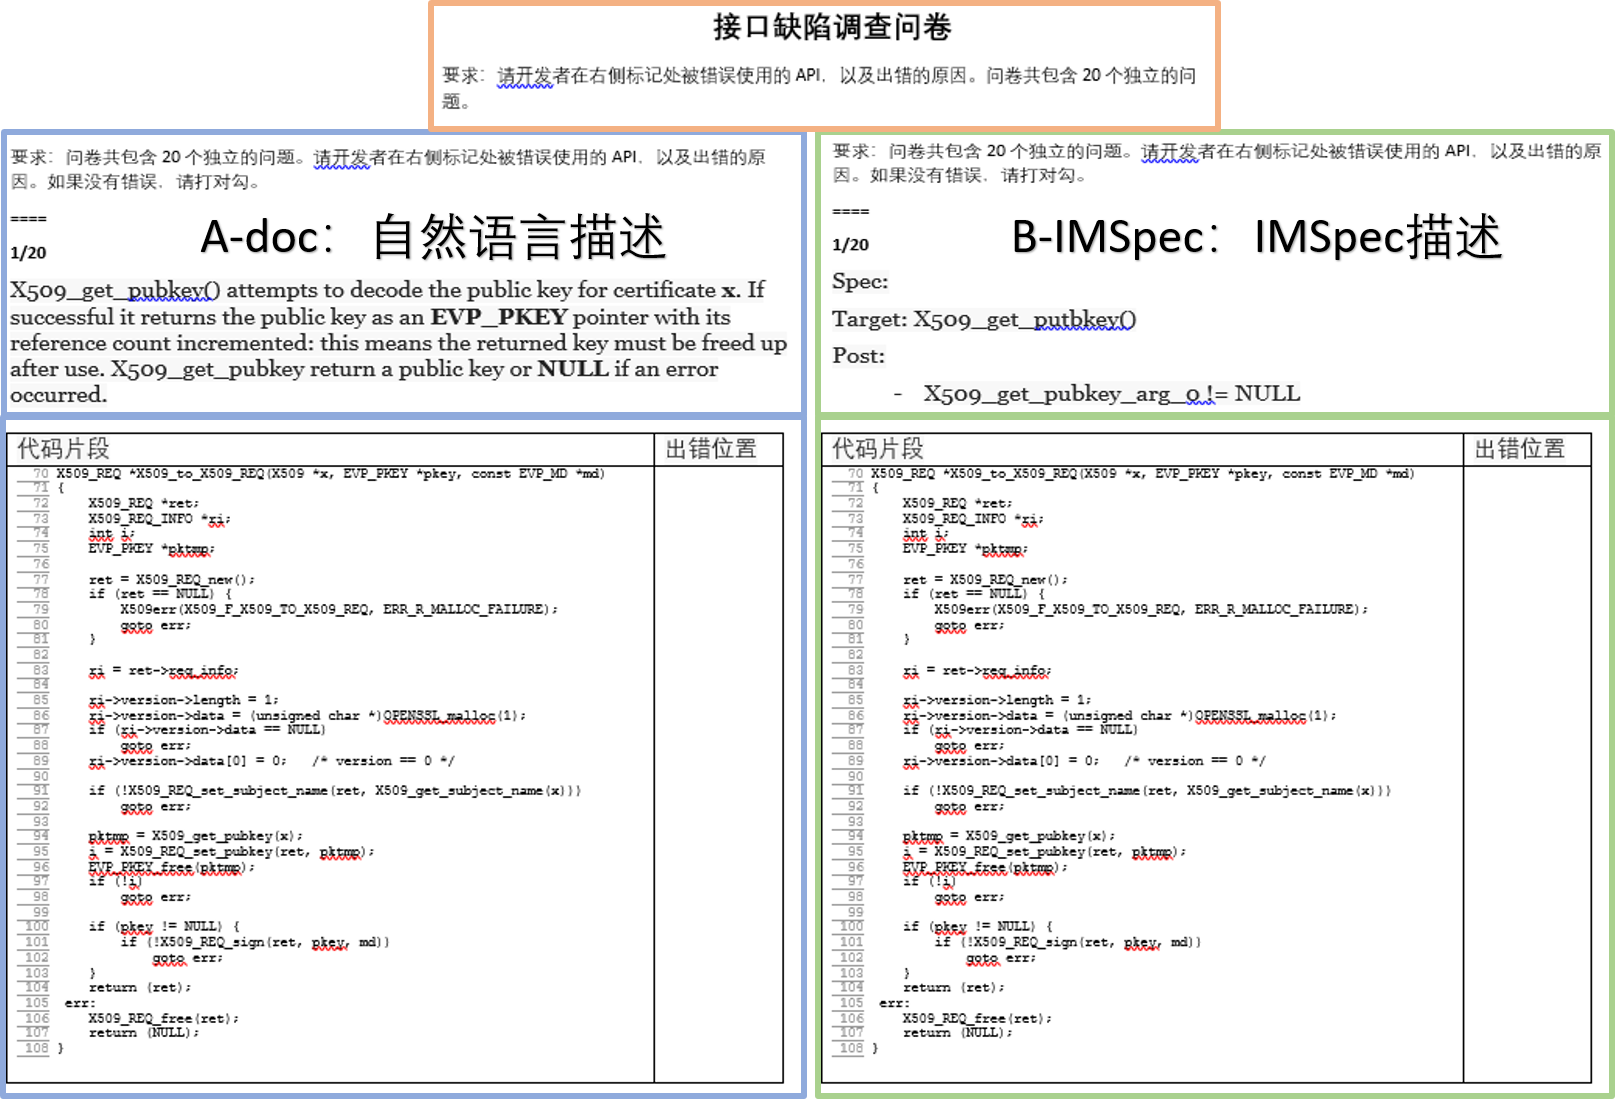
\includegraphics[width=0.85\linewidth]{figures/cp2-survey.png}
	\caption{
		接口缺陷检测调查问卷。
	}
	\label{fig:2-5-survey}
\end{figure}

\paragraph{方法}
针对于“有效性”,本文以实际开发者作为评估对象。
由于OpenSSL提供良好的接口使用用户手册~\footnote{https://www.openssl.org/docs/manmaster/man3/},
因此作者对OpenSSL的缺陷进行随机取样并用于评估。
在预实验中,作者对开发者一次能够接受的缺陷审查的数目进行调研。
结果显示5-10个是开发者能够接受的区间。
所以,作者将随机选择的10个缺陷实例与这些缺陷的修复版本随机排序。
并构造两组测试集:
A-doc组提供OpenSSL项目提供的自然语言描述的使用说明,
B-IMSpec提供基于IMSpec描述的使用约束。
通过随机选择的方式,每组测试集各发放给20名研究或者工作领域与测试、
程序分析等背景相关的实际开发人员。
对于A-doc组被测对象,作者对OpenSSL的背景进行介绍;
对于B-IMSpec组被测对象,作者对OpenSSL背景以及IMSpec进行了简单的介绍。
特别地,为B-IMSpec组提供图~\ref{fig:2-4-example}和图\ref{fig:2-4-example-imspec}作为参考资料。
作者请这些开发人员对代码中存在的缺陷进行标注,
如图\ref{fig:2-5-survey}中所示。
如果代码存在缺陷,请被测对象标注位置和原因;
如果没有则打对勾。
\begin{equation}
\label{eq:p}
P = \dfrac{\text{\# of 开发者报告中的真实缺陷}}{\text{\# of 开发者报告缺陷总数}}
\end{equation}
\begin{equation}
\label{eq:r}
R = \dfrac{\text{\# of 开发者报告中的真实缺陷}}{10}
\end{equation}


令包含误用的测试用例为真实缺陷。
对于开发人员的标注结果,从精度和召回率进行评估。
其中,精度的定义如公式\ref{eq:p}所示,
是被测对象找到缺陷中真实的缺陷个数与缺陷报告总数的比值。
较高的精度值表示缺陷检测效果误报率低,即找到的就是缺陷。
召回率的定义如公式\ref{eq:r}所示,是真实的缺陷与所有缺陷的商。
较高的召回率表示缺陷检测能力强漏报率低,即能够找到更多缺陷。


\begin{table}[b]
	\centering
	\begin{minipage}[t]{\linewidth} % 如果想在表格中使用脚注,minipage是个不错的办法
		\caption{基于两种描述方式的开发者审查结果}
		\label{tab:2-5-survey}
			\begin{tabular}{ccccccccc}
			\hline
			\multirow{2}{*}{实验组} & \multicolumn{2}{c}{问卷情况} & \multicolumn{2}{c}{测试集} & \multicolumn{2}{c}{平局缺陷报告情况} & \multicolumn{2}{c}{平均结果} \\
			\cline{2-9}
			& 发放 & 收回 & 缺陷数& 正确数& 报告总数 & 真实缺陷 & $P$ & $R$ \\
			\hline
		A-doc	& 20 & 13 & 10& 10& 3.92 & 3.69 & 94.13\% & 36.90\% \\
		 B-IMSpec	& 20 & 18 & 10& 10& 8.06 & 7.94 & 98.51\% & 80.60\% \\
			\hline
		\end{tabular}
	\end{minipage}
\end{table}

\paragraph{结果}
本文将针对于有效性的评估结果展示在表\ref{tab:2-5-survey}中。
在所有发放的调查问卷中,A-doc组共收回13份(65\%),
B-IMSpec组共收回18份(90\%)。
在问卷中,共包含10个正确的使用和10个错误的使用。
本文对于收到的调查问卷中的所有缺陷报告进行统计。
特别地,对于问卷中没有做出标记的用例,
本文认为是开发者没有能够找到该缺陷。
即认为是正确使用,效果等同于对勾。
如表中所示,A-doc组平均报告缺陷总数为3.92个,其中3.69个为真实缺陷;
B-IMSpec组平均报告缺陷总数为8.06个,其中7.94个为真实缺陷。
在统计后,本文对两组的开发者进行二次回访,
对没有回复的原因、缺陷定位的方法、误报和漏报的原因、缺陷分析中遇到的困难、
与自然语言相比IMSpec是否能够对接口使用约束描述更有效等问题进行调研。
在分析和比对后,作者总结如下。

{\kaishu 精度与召回率 }
如表\ref{tab:2-5-survey}中所示,两组的精度都很高。
其中A-Doc组的平均检测精度为94.13\%,B-IMSpec的平均检测精度为98.51\%。
该结果显示,测试人员对于自然语言和IMSpec都能够正确理解,
即两者对接口使用约束的条件的描述能力相同。
然而两组的召回率却存在较大差异,
其中A-doc组的召回率为36.9\%,比B-IMSpec组低43.7\%。
在对调查问卷本身和二次回访的结果进行分析和总结后,
本文发现,A-doc组13个返回结果的被测对象中,有10个并没有完全进行。
即,其后几个缺陷没有做出标记,也没有打对勾或者提供任何正确使用的标记。
该现象的一个主要原因是,测试人员对自然语言的描述失去耐心。
在二次回访中,作者将基于IMSpec描述发送给这些被测对象。
结果显示,开发者相比与自然语言,更愿意接着类程序语言的IMSpec。
因此,相对于自然语言,开发者认为IMSpec的描述有效性更好。
	
{\kaishu 被测对象遇到的困难 }
我们对被测对象遇到的困难、误报漏报的原因进行分析和总结。
结果显示,开发者在进行调研问卷的过程中,存在如下几个主要困难:
\begin{enumerate}
	\item 时间问题。
	在二次回访的过程中,A-doc组中有3位第一次没有回复的开发者进行解释。
	他们忽略该调研的主要原因有两个。
	一方面,20个测试用例太多,测试者认为需要大量的时间进行分析。
	另一方面,当看到自然语言描述的规约时,测试者更加放弃进行测试的想法。
	\item 结果不一致。
	在两种测试人员当中,绝大部分被测对象没有OpenSSL的开发经验。
	但是在提供接口使用约束的条件后,
	开发者能够对这些领域相关的API进行缺陷检测。
	然而,被测对象的结果存在两方面的不一致。
	一方面,同一个开发人员,对于同种缺陷模式,
	有的成功找到缺陷位置和原因、有的则没有找到。
	另一方面,同一个缺陷,有的开发者认为是缺陷、有的则认为不是缺陷。
	特别地,对于参数检查问题,不同的开发者理解不同。
	即,有的认为必须进行检查、有的认为可以不检查。
	\item 上下文信息不足。
	为节省篇幅以及对问卷长度的担心,
	本文每个测试用例只提供了目标API的单层函数的代码。
	特别地,对于长度过长的调用,进行程序截取。
	因此,两组测试人员都表示,很多情况下缺失的上下文信息影响了结果的判断。
	该影响主要表现在,召回率上。
\end{enumerate}
	
针对于IMSpec描述的有效性,
实际开发者表示该语言能够有效的描述接口使用约束。
同时,评估结果显示相对于自然语言,
IMSpec的表现形式更利于开发者理解接口使用约束。

\section{本章小结}
\label{sec:2.6}
本章提出基于缺陷模式的C程序接口使用约束领域特定语言。
为有效的进行语言设计,本章首先对C程序中的接口误用缺陷实例进行研究和总结。
以不同领域、广泛使用的六个开源软件作为研究对象,
对开发过程中出现的830个实际接口误用缺陷实例进行分析和归纳。
本章总结出三类常见接口缺陷模式,包括:
不正确的参数使用、不正确的异常处理以及不正确的因果调用关系。
这些缺陷模式有利于研究人员和开发者理解API误用缺陷的本质,
设计和开发更好的API,以及接口缺陷检测工具。
基于常见缺陷模式,
本章提出IMSpec领域特定语言,以描述C程序中接口使用约束,
并给出该语言的设计动机、语法结构和形式语义。
本章将IMSpec应用于实际项目的缺陷实例中。
应用结果表示该语言能够有效地描述实际项目中接口使用约束。

\chapter{接口缺陷静态检测技术研究}
\label{cha:imchecker}
软件库通过应用编程接口(API)来封装已有功能,提高开发效率。
正确的接口使用需要满足特定的约束,否则引入接口误用,导致接口缺陷。
静态检测技术是在不运行程序的前提下对程序的行为进行分析的技术,
能够在开发早期进行应用,
极大地降低缺陷修复的成本。
现有的静态检测技术可以分为两类,基于程序分析的缺陷检测技术和基于数据挖掘的缺陷检测技术。
虽然现有工作能够对实际缺陷进行检测,然而存在若干不足。
主要表现在,(1)缺陷模式难以扩展,对用户自定义的接口支持不足;
(2)语义分析不足,检测结果不精确。
特别地,随着现代软件规模大、结构复杂,以及开源代码的广泛使用,使得检测技术面临新的挑战。
因此,研究精准高效的C程序接口缺陷检测技术,对于提升软件系统可靠性和安全性具有重要意义。

本章旨在研究规模化接口缺陷静态检测技术,以对大规模程序中接口误用缺陷进行准确、高效的检测,
弥补现有静态检测技术不足。
本章首先基于第\ref{cha:imchecker}章的缺陷模式对现有工作进行分析,总结现有工作的特点和不足。
接着提出了基于规约描述的规模化接口缺陷检测技术IMChecker。
IMChecker通过IMSpec规约描述以支持多种缺陷模式和用户自定义的接口,
基于多入口分析策略以应对实际项目中大规模代码,并基于语义信息和统计信息对结果的精度进行提升。
从全文的研究体系上看,
本章的工作是规约描述语言IMSpec的应用,同时是接口缺陷检测实际应用的重要核心。

\section{引言}
开发者在利用API快速构建系统的同时,需要满足接口使用时的约束条件,以正确执行接口内部封装的功能。
否则将会产生接口误用,导致软件缺陷。
对接口误用检测进行研究具有重要意义。
一方面,接口误用是导致软件错误、系统崩溃、漏洞产生的重要愿意之一。
CWE组织2011年发布的最危险的25个软件错误中,有40\%和接口误用相关~\cite{cwe-top25}。
同时,OWASP项目在2017年发布的最危险的10个网络漏洞中,有30\%和接口误用相关~\cite{owasp-top10}。
另一方面,随着开源社区的发展,软件库文档缺失、开发人员对API理解不足,
导致现有的代码中存在大量的接口误用缺陷。

近年来,研究人员设计并实现了各种各样的方法来检测接口缺陷。
特别地,静态检测技术获得广泛的关注和应用。
静态检测技术能够在不执行代码的情况下进行分析。
所以,可以应用于开发的各个阶段,有效的提高代码质量。
同时,静态分析在使用时不需要人工标记、构造测试用例和测试环境。
因此,能够对所有的程序路径进行模拟执行,使用范围广。
针对于接口缺陷检测,从分析策略上来说静态分析包含两种主要的技术路线:
程序分析技术~\cite{16-saner-evaluation}和数据挖掘技术~\cite{survey18}。
基于程序分析技术的检测方法和工具需要研究人员和工具实现者的领域知识,
通过规约描述或者程序硬编码的方式对目标接口使用的约束进行定义。
此后,基于程序语义,通过可达性分析、程序语义匹配等方式进行缺陷检测。
基于数据挖掘技术的方法和工具则通过统计学习的方法,根据算法设计者预定义的模式在项目中进行接口使用约束推理。
此后,基于推理的约束基于统计意义进行缺陷检测。

虽然,两者都能够在实际项目中进行应用并找到新的缺陷。
然而,两者存在两个主要不足:
(1)缺陷模式难以扩展,对用户自定义的接口支持不足。
前者无法应用于未定义的目标API,后者则依赖于大量高质量的数据以学习正确的约束。
(2)语义分析不足,分析精度不够,难以应用于实际项目中。
一方面,现有的工具多基于语法层分析;另一方面,为了支持大规模代码,
工具多在过程内分析,忽略了过程间的语义信息。


为解决上述方法中的不足,本章提出了基于规约描述的规模化接口缺陷静态检测方法IMChecker。
首先,IMChecker通过IMSpec规约描述以支持多种缺陷模式和用户自定义的接口。
精度和效率是静态分析技术需要平衡的重要指标。
高精度的分析技术需要昂贵的计算代价,从而限制了静态分析在实际项目上应用效果。
高效率的分析技术则存在分析精度的损失,产生大量的误报(False Positive, 将正确行为报告称缺陷)
和漏报(False Negative,实际缺陷没有被检测出)。
因此,基于多入口分析策略,将复杂的程序分析问题分而治之,高效率分析的同时,
实现局部的精确分析。
针对于多入口分析策略导致的分析精度的损失,
IMChecker通过基于上下文的语义摘要信息和基于使用情况的统计信息进行结果过滤,
以提交检测的精度。
本章基于目前已知最大规模的开源缺陷测试集Juliet Test Suite中,13个接口缺陷相关的CWE分类对IMChecker方法进行评估。
实验结果显示,IMCHecker方法误报率为13.21\%,漏报率为16.08\%。
检测能力领先于主流的开源软件项目。

本章其余部分组织结构如下:
\ref{sec:3.2}节对相关研究进行总结;
\ref{sec:3.3}节对规模化接口缺陷静态检测算法进行介绍;
\ref{sec:3.4}节给出工具评估和研究评估结果;
最后在\ref{sec:3.5}节总结本章工作。
\section{相关工作}
\label{sec:3.2}

静态缺陷检测方法在不执行程序的情况下,对程序中的缺陷进行检测。
针对于C程序接口缺陷,近年来,研究人员和工具开发者设计并实现了各种各样的静态检测算法和工具~\cite{16-saner-evaluation, survey18}。
本节对其中的典型算法和工具进行调研和总结。

从技术路线上来说,静态缺陷检测方法可以分为两大类,
\begin{itemize}
	\item {\kaishu 程序分析技术}程序分析技术需要明确的提供目标接口的使用约束。
	因此需要研究人员和开发者具有良好的领域知识。
	目前,约束的描述方式有两种:规约描述语言和程序硬编码检测器。
	前者在分析的过程中,首先将语言进行解析并构造监控自动机的中间表达。
	在程序语义分析阶段,通过可达性分析对缺陷进行检测。
	该方法有利于对新的接口进行扩展,即提供对应的缺陷描述。
	后者则在分析的过程中,基于程序语义进行模式匹配对缺陷进行检测。
	该方法难以扩展,需要实现新的检测器。
	基于程序分析技术的工作,最大的优点是可以有效利用积累的领域知识,以及利用语义分析获得更加准确的分析结果。
	\item {\kaishu 数据挖掘技术}数据挖掘技术则不需要用户提供显示的约束,
	可以基于统计信息,基于学习的方法自动推理约束。
	其检测的核心在于,通过对程序形式的转化,构造中间表达。
	并基于预先定义的模式,基于统计信息学习接口使用的约束。
	特别地,大多数方法认为:多数使用为正确用法,少数为错误。
	虽然基于数据挖掘技术的检测方法不要人定义具体的约束,
	但是需要良好领域知识设计学习模型。
	因此,其扩展性交叉。
	基于数据挖掘技术的工作,最大的优点是设计好学习模型后可以实现完全自动化,同时不需要项目特定的领域知识。
\end{itemize}

具体来说,如表~\ref{tab:3-2-survey}中所示,本文共对17个研究工作和工具进行调研的总结。
其中前五个为基于程序分析技术的普适性静态缺陷检测工具,包括开源软件三个,以及两个商业工具的学术使用版。
第6-7个为针对接口设计的基于程序分析技术的静态缺陷检测工具。
最后10个则为基于数据挖掘技术的程序接口缺陷检测技术。
针对于提供工具的工作,作者对工具进行使用;
对于没有工具的工作,作者对论文进行阅读,总结其检测能力。
特别地,为了减少作者的主观臆断带来的影响。
对于每一个工作,作者或直接和论文作者进行结果核对,或同时阅读了3-5个引用该论文的其他工作,与这些论文中的描述进行核对。

\begin{table}[t]
	\centering
	\begin{minipage}[t]{0.85\linewidth} % 如果想在表格中使用脚注,minipage是个不错的办法
		\caption{静态分析工具对C程序接口缺陷检测能力}
		\label{tab:3-2-survey}
			\begin{tabular}{@{\extracolsep{3pt}}ccccccccccc@{}}
			%\begin{tabular}{ccccccccccc}
			\hline
			\multirow{2}{*}{工具名称} & \multicolumn{2}{c}{IPU\footnote{Y:支持,P:部分支持,-:不支持}} & \multicolumn{3}{c}{IEH} & \multicolumn{3}{c}{ICC} & \multirow{2}{*}{扩展性\footnote{难:难以扩展,有限:可以扩展,扩展内容受限,-:不支持,$\checkmark$:方便扩展}} & \multirow{2}{*}{可用性\footnote{$\checkmark$:可用且基本符合预期,P:可用但与预期相差很大,-:不可用}} \\
			\cline{2-3}\cline{4-6}\cline{7-9}
			 & -s & -r & -c & -p & -l & -s & -c & -r & & \\
			\hline
			Clang-SA~\cite{clang-sa} & Y & Y & - & - & - & Y & Y & Y & 难 & $\checkmark$ \\
			Cppcheck~\cite{cppcheck} & Y & Y & P & - & P & Y & Y & Y & 有限 & $\checkmark$ \\
			Infer~\cite{infer} & Y & Y & - & - & - & Y & Y & Y & - & $\checkmark$ \\
			Pinpoint~\cite{pinpoint} & Y & Y & P & - & - & Y & Y & Y & - & $\checkmark$ \\
			Coverity~\cite{coverity} & Y & Y & Y & P & P & Y & Y & Y & 难 & $\checkmark$ \\
			\hline 
			SLAM~\cite{slam} & Y & Y & Y & - & - & Y & Y & Y & 有限 & $\checkmark$ \\
			SSLINT~\cite{15-sp-sslint} & P & - & Y & - & - & Y & Y & - & 有限 & - \\
			\hline
			PR-Miner~\cite{05-fse-prminer} & - & - & - & - & - & Y & Y & - & - & - \\
			RGJ07~\cite{07-PLDI-RGJ07} & Y & Y & - & - & - & Y & Y & - & - & - \\
			Chronicler~\cite{07-icse-chronicler} & - & - & - & - & - & Y & P & - & - & - \\
			EDP~\cite{08-fast-eio} & - & - & Y & Y & - & - & - & - & - & - \\
			Hector~\cite{13-dsn-hector} & - & - & - & - & - & Y & P & - & - & - \\
			Chucky~\cite{13-ccs-chucky} & P & P & Y & - & - & - & - & P &  & \checkmark \\
			NDNR14~\cite{14-fse-pre} & P & Y & - & - & - & - & - & - & - & - \\
			APISan~\cite{16-sec-apisan} & P & P & Y & Y & - & Y & Y & P & - & \checkmark \\
			Antminer~\cite{16-icse-antminer}& P & P & Y & P & - & P & P & - & - & - \\
			ErrDoc~\cite{17-fse-errdoc}& - & - & Y & Y & P & P & - & - & 有限 & P \\
			\hline
		\end{tabular}
	\end{minipage}
\end{table}
如表~\ref{tab:3-2-survey}中所示,本文从三个方面共对17个研究工作和工具进行调研的总结。
即,检测能力、扩展性和可用性。
表中第一列为项目名称。
第2-9列,为工具对于第~\ref{sec:2.3}节中总结实际项目的缺陷模式的支持情况。
特别地,IPU-s代表单个参数的检查、IPU-r代表参数之间和参数与返回值之间的检测;
IEH-c代表异常处理中对接口返回值的检测、IEH-p为异常处理中返回错误代码的检测(error propagation)、
IEH-l为异常处理中对缺陷信息打印支持的检查;
ICC-s为不带上下文关系的接口对、ICC-c为带有上下文关系的接口对、ICC-r代表重复调用的检测。
第10列扩展性关注,算法和工具是否能够针对用户需求预留了扩展的接口,对项目特定的接口检测进行扩展。
其中难表示可以扩展,但是代价非常大,比如Clang-SA需要重新设计检查器插件;
有限代表工具提供了扩展的方式,但是扩展的内容需要满足特定的缺陷模式。
最后一列为工具的可用性,即该工具是否可用。
特别地,工具的效果是否和发表的论文、工具说明一致。
其中,P代表工具可以下载和使用,但是其功能和论文描述不符。
即,工具难以支持论文中明确给出的代码样例。

检测能力方面,
从表中调研结果可知,在所有的工作中,并没有一个工作能够完全的支持所有的接口缺陷模式。
特别地绝大多数基于数据挖掘技术的工作,只能处理某一种特殊的缺陷模式。
检测能力最好的是商业工具Coverity和基于数据挖掘技术的工具APISan。
然而前者实际价格昂贵,难以广泛使用。
后者基于数据挖掘技术,工具作者在论文中指出,具有极高的误报率。
此外,在所有缺陷模式中,单个参数检查、异常处理中返回值检查和
不带有上下文语义关系的函数调用对检查被大多数工具支持。
这些缺陷模式相对简单,能够从语法结构直接进行检查。
然而,本文作者发现,绝大部分工具并没有考虑足够的语义信息。
例如,对于参数的检查,如果缺少参数或者代码中参数与常量比较则工具支持效果较好。
但是如果比较的方式为和变量比较,则工具存在大量漏报。

扩展性方面,只有6个工具提供了扩展的接口。
其中Clang-SA和Coverity需要设计新的检测器插件,扩展难度极大。
SLAM、SSLINT、Errdoc可以通过撰写规约的方式对检测目标扩展,然而其只能针对于特定的缺陷模式或者项目特定的接口扩展。
即SLAM针对于Windows操作系统内核的驱动程序设计,SSLINT针对于SSL/TLS安全协议设计和
Errdoc针对于异常处理设计。
Cppcheck为用户提供了最方便的扩展接口。
通过提供结构化的接受使用描述方式,用户可以对自定义的接口进行扩展。
然而,Cppcheck提供的语言只能够支持单个参数、参数关系、返回值检测和不带因果关系的函数对四种情况。

应用性方面,基于数据挖掘的工作中可用的工具只有Chucky和APISan。
Errdoc工具在适用时,作者发现其与论文描述差距较大。
基于程序分析技术的工具作者选择的都是可以使用工具,因此实用性较好。
然而,在实际项目应用中,作者发现,这些工具的分析报告存在两种极端的表现。
即要么报告数量多,但存在大量的误报;要么报告数极少,与其他工具项目,存在大量的漏报。

总体来说,针对于C程序接口缺陷检测,现有的工作存在两点主要不足。
(1)缺陷模式支持有限,扩展性不足,难以支持用户自定义的接口。
一方面,基于程序分析的技术需要通过规约撰写或者开发新的检测插件。
如第~\ref{sec:2.2}和本章调研结果所示,现有的约束描述方法或过于复杂,或难以扩展到全部接口缺陷模式。
同时,开发新的插件则需要理解工具框架和细节,难以实际使用。
另一方面,基于数据挖掘的技术需要大量可靠数据进行约束学习。
然而,该需求对于独立的项目难以实现。特别地,用户自定义的接口往往使用次数有限,
难以满足学习所需要的数据量。
(2)语义分析不足,检测结果存在大量误报和漏报,难以支持实际项目分析。
一方面,为了提高缺陷检测的效率,现有的工具多基于语法结构对缺陷分析。
因此,难以支持需要语义信息的缺陷。
另一方面,多数工具基于过程内分析策略,以应对大规模程序。
然而,丢失的上下文语义信息,会导致误报和漏报。

\section{接口缺陷静态检测算法}
\label{sec:3.3}
本节提出IMChecker,以解决上述不足。
通过 1 2 3 来做什么


(seke19)
我们以图1.1中的例子作为案例,

介绍总体图和流程

每部分的主要工作
1.5页

\subsection{构造分析上下文}
编译抓取,为什么IR

介绍CFA,给一个图
1页

对于命令式语言的程序可以用控制流自动机(Control-flow Automaton,CFA) cxP3.3.1

多入口分析策略cx89
0.5页

函数展开
循环
0.5

\subsection{抽象符号路径提取}
语法

解释用例子

结果
1.5页
\subsection{缺陷检测算法}
算法
1页
例子解释
0.5页

%\begin{algorithm}
	\KwIn{~~~\textsf{SyncBlock} 计算模型内所有复合构件的 $<connection>$,
		\\~~~~~~~~~~~~~~~顶层复合构件的所有输入端口 $<port\_declaration>$,
		\\~~~~~~~~~~~~~~~顶层的每一个输入端口 $p_i$ 对应的环境输入值 $I_i$。 }
	\KwOut{更新所有与顶层复合构件输入端口相连接的端口的值。}
	\vspace{3ex}
	%\SetAlgoLined
	\For{~~顶层复合构件 $<port\_declaration>$ 中的每一个输入端口 $p_i$~~}{
		$p_i \gets I_i$ \;
		\tcp{取出所有与 $p_i$ 直接相连的内部子构件的端口}
		$p_i \left[\right] \gets Connection\_Target(p_i,~<connection>)$ \;
		\For{~~$p_i \left[\right]$ 中的每个端口 $p_i\left[ j \right]$~~} {
			\tcp{根据端口 $p_i\left[ j \right]$ 的性质,判断是否要继续向下搜索传递}
			\eIf{~~$p_i\left[ j \right]$ 不是原子构件的输入端口~~}{
				\tcp{如果连接上有表达式,进行数据处理再赋值}
				\eIf{~~$<connection>$~上有表达式~~}{
					$p_i\left[ j \right] \gets Comput\_Exp(p_i)$ \;
				}{
					$p_i\left[ j \right] \gets p_i$ \;
				}
				\tcp{取出所有与$p_i\left[ j \right]$ 直接相连的端口,添加到 $p_i \left[\right]$ 中}
				$p_{temp} \left[\right] \gets Connection\_Target(p_i\left[ j \right], <connection>)$ \;
				$p_i \left[\right] \gets Append(p_i \left[\right], p_{temp} \left[\right])$ \;
				
			}{
				\tcp{$p_i\left[ j \right]$ 是原子构件的输入端口,不需要继续向下搜索传递}
				\eIf{~~$<connection>$~上有表达式~~}{
					$p_i\left[ j \right] \gets Comput\_Exp(p_i)$ \;
				}{
					$p_i\left[ j \right] \gets p_i$ \;
				}
			}
			
		}
	}
	\caption{从外部环境读入输入序列,传递到原子构件输入端口}
	\label{alg:Input}
\end{algorithm}


\subsection{检测结果过滤}
为什么

语义例子

统计例子
1.5页
\section{工具实现与实验评估}
\label{sec:3.4}
本节首先介绍规模化接口缺陷检测方法IMChecker的实现细节。
随后在公开数据集上,对IMChecker的分析能力进行评估,并给出IMChecker与主流开源工具的比较结果。

\begin{figure}[t]
	\centering
	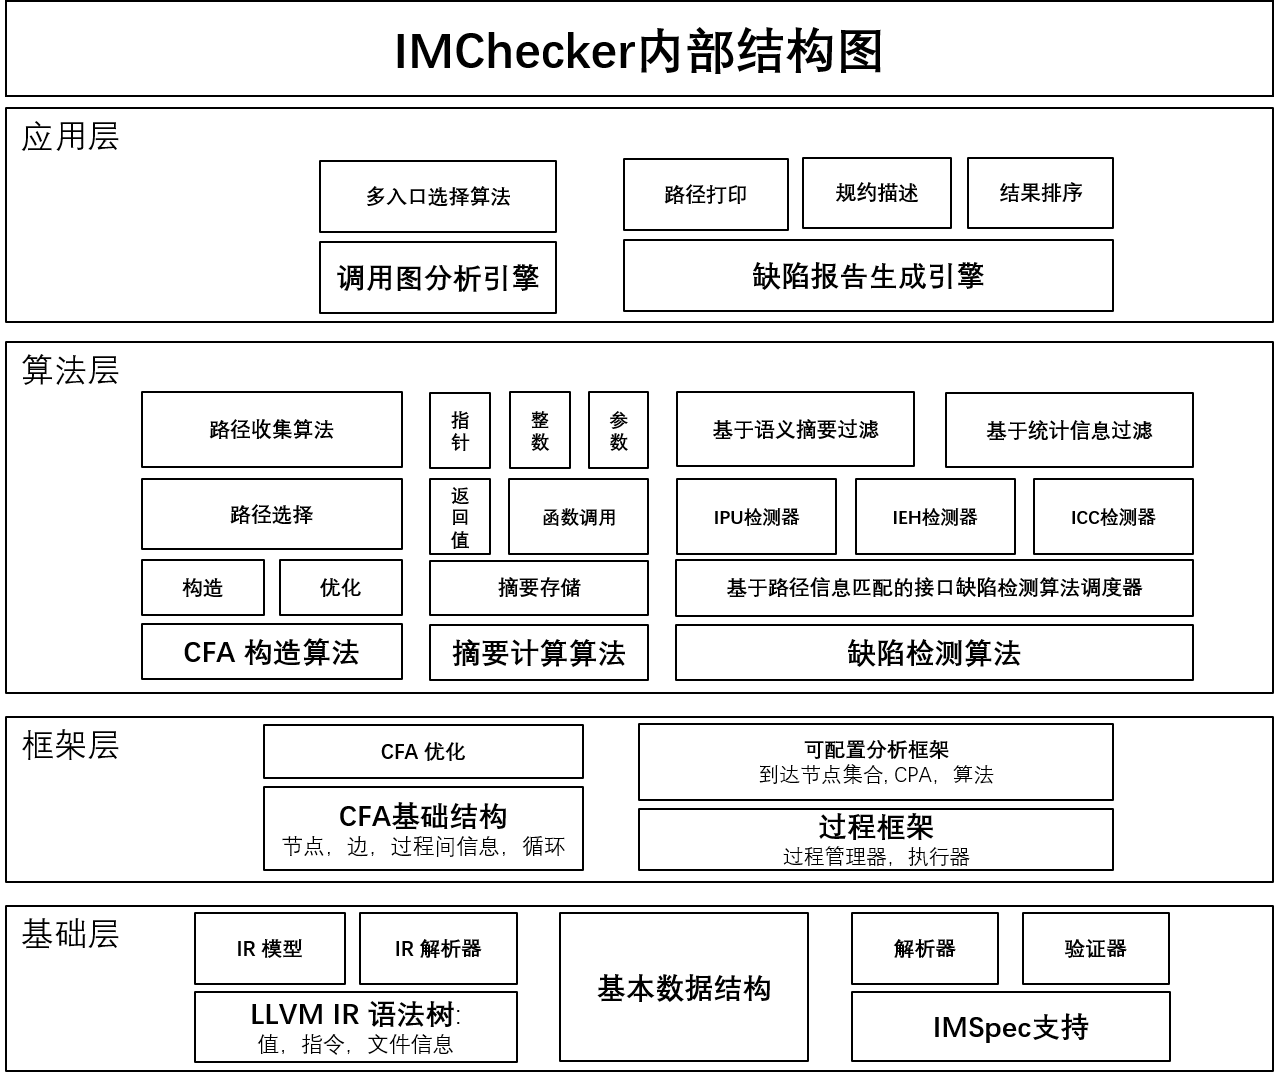
\includegraphics[width=0.9\linewidth]{figures/cp3-implementation.png}
	\caption{
		IMChecker工具内部结构图
	}
	\label{fig:3-4-implementation}
\end{figure}

\subsection{工具实现}
IMChecker基于Java语言实现,依赖于LLVM3.9的IR作为分析的中间表达,
并基于CPA~\cite{07-cav-cpachecker}算法作为整体方法的实现基础。
工具接口用户提供的源代码和IMSpec规约描述作为输入。
其中IMSpec实例和缺陷检测结果都基于Yaml~\cite{yaml}格式存储。
工具实现的内部结构如图~\ref{fig:3-4-implementation}所示。
工具共包含四个层次:基础层、架构层、算法层和应用层。
首先,基础层通过对源代码处理,生成LLVM-IR中间表达;并对IMSpec规约描述进行解析和一致性分析。
架构层构造CFA,将程序转化为图结构;
同时,提供基于CPA算法的分析流程以支持上层语义计算的算法。
算法层,则对CFA进行优化、计算语义摘要信息以及缺陷检测。
最后,应用层通过调用图具体进行分析入口的选择,执行缺陷分析;
并将缺陷检测的结果进行过滤、排序和信息打印。

\paragraph{基础层}
基础层旨在对用于输入的源代码和IMSpec规约描述进行预处理,同时提供分析中需要的基本数据机构。
首先,针对于用户输入的源代码,
如果待测程序是单个的C文件,IMChecker直接使用clang编译器
\begin{lstlisting}[language={bash},
basicstyle=\linespread{0.8}\listingsfont,
numbers=none,
xleftmargin=.25\textwidth]
(*@\textcolor{blue}{Ubuntu@~: clang}@*) path2source -S -emit-llvm -g
\end{lstlisting}
进行预处理以生成自包含的.ll文件。
该文件相比于原.c文件增加了必需的函数和数据结构声明,展开了宏定义,消去了预处理指令等。
同时生成了对应的LLVM-IR中间表达。
如果待测程序是一个Makefile工程,
那么通过解析Makefile中的编译指令并且将所有输出.o文件的指令替换为相应的预处理指令,例如clang -E。
预处理生成的.i文件,再利用上述指令生成.ll文件。
同时,根据Makefile的编译目标,项目被组织成不同的分析任务。
通过llvm的链接指令(llvm-link)将给定分析任务下所有的.ll文件进行合并,
作为输入进行缺陷检测。
在获得LLVM-IR中间表达后,利用javacpp\footnote{https://github.com/bytedeco/javacpp}工具解析文件,
并构造IR模型,包括值、指令和文件信息。
另一方面,基础层对用户提供的IMSpec语言进行解析。
IMSpec语言针对于单个目标API设计,所以如果规约中存在语法错误则将错误规约忽略并输出给使用者。
同时,解析后的IMSpec进行语义一致性验证,即是否存在冲突的约束。
例如,一个条件未接口的第一个参数大于零,另一个条件未第一个参数小于零等等。

\paragraph{框架层}
框架层旨在提供分析框架的实现以及基本土结构的创建。
在对用户提供的源代码解析过后,CFA基本结构模块对LLVM-IR进行包装,构造CFA结构。
特别地,CFA在节点上表示程序的位置,在边上封装程序的具体执行指令。
为了在CFA图上提供更多的语义信息,
本文将CFA边分为两种,即控制边和摘要边。
前者表示具体的语义操作的指令,例如存储、运算、返回等等。
后者表示函数调用和循环关系。
因此,通过摘要边,在分析中可以利用摘要信息跳过函数展开和循环遍历,
在保证大规模代码有效分析的同时增加分析精度。
IMChecker基于过程(Phase)来运行,即每个过程复杂不同的预处理或者检测步骤。
所以,框架层中实现了过程管理的调度器。
特别地,IMChecker基于CPA算法来实现具体的路径抽取和缺陷检测。
因此IMChecker在框架层实现了CPA算法的核心数据结构和基础调度算法。
具体的每一个CPA则在算法层中实现。

\paragraph{算法层}
算法层旨在实现具体的算法细节。
IMChecker针对C程序接口使用缺陷进行检测,在整个分析过程中可以分为三个阶段:
路径收集、摘要计算和缺陷检测。
\begin{itemize}
	\item {\kaishu 路径收集} 在路径收集阶段,IMChecker利用CFA构造算法,对框架层的CFA原型进行优化。
	特别地,为了支持大规模程序分析,IMChecker基于入口分析。
	因此,在这个阶段对入口进行标记。
	此后,基于优化后的CFA图结构,通过第~\ref{sec:3.3}节中的路径抽取方法,
	收集路径信息,为后续两个步骤做准备。
	目前IMChecker基于AccesPath~\cite{15-ase-accesspath}和整数分析对语义信息进行计算。
	\item {\kaishu 摘要计算} 
	摘要计算的结果应用于缺陷检测当中,在实现上,IMChecker则先进行摘要的计算。
	为了支持大规模程序检测,IMChecker采用了基于多入口分析的策略,使得分析精度下降,
	导致大量误报。
	为了提供更加准确的检测结果,IMCHecker利用上下文语义信息对结果进行过滤。
	具体而言,IMChecker计算:上下文指针常量计算、整数常量计算、参数约束关系、
	返回值常量关系和函数调用关系的摘要信息。
	\item {\kaishu 缺陷检测} 
	缺陷检测部分,IMChecker实现了基于路径信息匹配的接口缺陷检测算法。
	特别地,为了提高检测精度,IMChecker实现了检测算法调度器。
	即,根据使用约束的不同,调用不同的检测算法的实现,以精确分析程序进行缺陷检测。
	最后,利用基于语义的摘要信息和基于使用情况的统计信息对结果过滤。
\end{itemize}


\paragraph{应用层}
应用层旨在从方法实际程序运行的角度,对IMChecker进行封装和优化。
一方面,应用层实现了多入口选择算法和调度引擎。
通过该模块,具体执行每个入口的分析。
另一方面,对于检测后的缺陷,生成相应的缺陷报告。
包括,缺陷产生的路径信息、违反的规约描述和具体约束条件的IMSpec形式和自然语言解释。
特别地,IMChecker基于使用情况对缺陷检测结果进行排序。
目前,在满足最低使用次数(Minimum Support)的情况下,
IMChecker认为误用次数与使用次数的比例越小(Confidence)。
即该缺陷与大多数使用不一致,则该检测结果越有可能是缺陷。

IMChecker已经集成在Tsmart工具集中~\cite{tsmart},工具使用的具体细节将在第~\ref{sec:4.3}中进行介绍。

\subsection{实验准备}

\paragraph{测试集} 由于目前并没有针对C程序接口缺陷检测的测试集合,
因此作者基于美国国家标准技术研究所(NIST) 整理的Juliet Test Suite测试集~\cite{juliet},
对IMChecker的分析能力进行评估。
该测试集合包含超过6万个C/C++用例,涵盖118个不同的CWE缺陷类型,
是目前最为广泛使用的测试集。
本文根据接口缺陷模式共选取了13个具体的分类。
Juliet测试集合每个分类中给出了大量的重复模式的测试用例,和不同的产生原因。
因此,作者对其中重复的用例进行过滤,保留由于接口误用导致错误的测试用例。
同时,对每个分类中的缺陷实例进行过滤和修正,
以确保其函数至少一个误用和一个修复后的版本。
如表~\ref{tab:3-4-cwe}所示,针对于第~\ref{sec:2.3}中总结的三大类接口误用模式,
共选取了2172个测试用例。
为了方便研究人员和开发者理解缺陷模式和评估检测工具,
本文将这些修订后的测试用例集成到APIMU4C,C程序接口误用数据集中。
APIMU4C将在第~\ref{sec:4.2}详细介绍。


\begin{table}[t]
	\centering
	\begin{minipage}[t]{0.8\linewidth} % 如果想在表格中使用脚注,minipage是个不错的办法
		\caption{评估测试集组成}
		\label{tab:3-4-cwe}
		\begin{tabular}{cccl}
			\hline
			{缺陷类别 } & {CWEID} & 缺陷数目 & \multicolumn{1}{c}{缺陷描述} \\
			\hline
			\multirow{6}{*}{IPU} & 121 & 36 & 栈内存越界读取\\
			& 122 & 36 & 堆内存越界读取 \\
			& 131 & 42 & 不正确的计算缓冲区大小\\
			& 476 & 36 & 空指针引用\\
			& 590 & 360 & 释放非堆内存\\
			\cline{2-4} 
			& \multicolumn{3}{c}{5个CWE分类,510个测试用例} \\
			\hline
			\multirow{3}{*}{IEH} & 252 & 270 & 未检查错误状态代码\\
			& 253 & 270 & 错误状态代码检查不正确\\
			& 390 & 72 & 未进行异常处理\\
			\cline{2-4} 
			& \multicolumn{3}{c}{3个CWE分类,612个测试用例} \\
			\hline
			\multirow{5}{*}{ICC} & 401 & 474 & 内存泄漏\\
			& 404 & 24 & 不正确的资源释放\\
			& 415 & 120 & 重复释放\\
			& 690 & 384 & 未对因果调用中的上下文关系检测\\
			& 775 & 48 & 未释放文件资源\\
			\cline{2-4} 
			& \multicolumn{3}{c}{5个CWE分类,1050个测试用例} \\
			\hline
		\end{tabular}
	\end{minipage}
\end{table}

\paragraph{ 比较对象}
首先,为了检测过滤机制的效果,本文将未添加过滤机制的方法记作为IMChecker--。
通过IMChecker与IMChecker--在测试集上的表现差别,以评估过滤算法的有效性。
此外,本文选取广泛使用的代表性开源工具进行检测能力的比较。
在对工具描述文档、学术论文和预实验后,本文选取了如下三个工具:
\begin{itemize}
	\item APISan~\cite{16-sec-apisan}(主分支-2018-0601):
	该工具是一个开源的学术工具,针对于接口误用缺陷设计。
	通过数据挖掘技术与程序分析技术结合,利用轻量级语义分析方法获得接口使用上下文信息,
	并基于统计方法推理接口使用约束。
	工具基于过程内分析方法,考虑函数返回值、参数关系和因果调用关系,并将规约推理的结果用于缺陷检测。
	不过,推理的结果没有输出,也没有提供扩展规约推理方法或者接受约束的接口。
	\item Cppcheck~\cite{cppcheck}(版本1.83):
	Cppcheck是针对于未定义和危险程序结构的缺陷检测工具。
	该工具开源代码,并支持多个领域和不同的缺陷类型。
	将代码转化为字节流(token)后,
	基于上下文敏感(context-sensitive)和流敏感(flow-sensitive)的过程间分析方法,
	对缺陷进行模式匹配。
	Cppcheck在检测算法中集成了C标准库的接口。
	同时,为了支持用户自定义的接口,提供了一套规约描述方法\footnote{http://cppcheck.sourceforge.net/manual.pdf, chapter10, page 20.},以利用实现过算法对相同的缺陷模式进行检测。
	例如参数空指针,内存泄漏等等。
	\item Clang-SA~\cite{clang-sa}(版本RELEASE\_600):
	该工具是LLVM开源编译器的组成部分。
	通过符号执行技术,推理程序语义。
	该工具采用上下文敏感(context-sensitive)和流敏感(flow-sensitive)的过程间分析方法,
	并实现了大量的检测插件,以应对不同的缺陷类型\footnote{http://clang-analyzer.llvm.org/available checks.html}。
\end{itemize} 
一方面,这三个工具提供了良好的缺陷报告接口,支持多种接口缺陷类型。
另一方面,这三个工具基于不同的分析技术(数据挖掘、静态分析-硬编码、静态分析-基于规约描述)。
同时,三个工具在预实验中的检测能力稳定,与文档论文中的描述能力一致。

\paragraph{评测指标}
在测试集上,本文将采用如下三个指标对工具进行评估。
\begin{itemize}
	\item 召回率(Recall):$R = \dfrac{\text{结果报告中真实的缺陷数}}{\text{总缺陷数}}$
	召回率是基于具体实现情况下,工具的检测能力。即,工具能够有效的检测多少缺陷。
	缺陷检测领域普遍认为,一个工具在测试集合上的召回率越高,那么其实际应用中也会有更好的检测效果。
	\item 精度(Precision):$P = \dfrac{\text{结果报告中真实的缺陷数}}{\text{工具报告的缺陷总数}}$
	研究表明,困扰实际用户使用静态分析的原因之一就是,现有的工具产生了大量的误报,即精度太低~\cite{10-acm-precision}。因此,检测工具的精度是重要的指标之一。
	特别地,如果精度低于30\%,那么实际使用者将抛弃这个工具。
\end{itemize}
%\item 理想召回率(Conceptual Recall,CR):$= \dfrac{理想情况下能够支持的缺陷数}{工具报告的缺陷总数}$
%该指标表示工具能够支持的最大程序的检测能力。即,工具用户手册或者论文中,不考虑实现的正确性下,提到能够解决问题的全部空间。一个工具的CR越高,代表这个工具的检测能力越强。 $R = \frac{结果报告中真实的缺陷数}{总缺陷数}$

\paragraph{运行环境} 本文在一台装有64 位Ubuntu 16.04的台式机上进行实验。
该机器配有Intel(R) Core(R) i5-3470@3.20GHz-4核心CPU和32GB内存。
本章关注接口缺陷检测的能力,因此不设置最长分析时间。


\subsection{评测结果}

\begin{table}[b]
	\centering
	\begin{minipage}[t]{0.9\linewidth} % 如果想在表格中使用脚注,minipage是个不错的办法
		\caption{IMChecker评测结果}
		\label{tab:3-4-imchecker}
		\begin{tabular}{cccccccccc}
			\hline
			\multirow{2}{*}{类别 } & \multirow{2}{*}{个数} & \multicolumn{4}{c}{IMChecker} & \multicolumn{4}{c}{IMChecker-~-} \\
			\cline{3-10}
			 & & 报告数 & TP\footnote{TP:真实缺陷数目} & P(\%) & R(\%) & 报告数 & TP& P(\%) & R(\%) \\
			 \hline
			 IPU & 510 & 490 & 423 & 86.33 & 82.94 & 745 & 469 & 62.95 & 91.96 \\
			 IEH & 612 & 580 & 506 & 87.24 & 82.68 & 677 & 526 & 77.70 & 85.94 \\
			 ICC & 1050 & 1012 & 878 & 86.76 & 83.62 & 1320 & 898 & 68.03 & 85.52 \\
			 总计 & 2172 &  2082 & 1807 & 86.79 & 83.20 & 2742 & 1893 & 69.04 & 87.15 \\
			\hline
		\end{tabular}
	\end{minipage}
\end{table}
\paragraph{IMChecker评测结果}
评测结果如表~\ref{tab:3-4-imchecker}中所示,
其中报告数为工具缺陷的总报告数,TP为报告中真实存在的缺陷数目,P为精度,R为召回率。
表中3-6列为IMChecker的评估结果,7-10列为IMChecker--的评测结果,即不包括过滤机制的结果。

评测结果表明,在所有的测试用例中,
IMChecker--共产生2742个缺陷报告,其中1893个为真实的缺陷,
849个为误报,平均精度为69.04\%,平均召回率为87.15\%。
在对缺陷报告深入分析后,导致IMChecker--分析结果不准确的主要原因是跨函数的接口使用。
如第~\ref{sec:3.3}中所示,为了能够支持大规模代码有效分析,IMChecker的检测算法基于过程内分析进行。
因此,当接口使用跨函数时,则会导致分析精度下降。

我们通过\texttt{malloc/free}例子进行分析。
在C的标准库中,两者组合进行堆内存的申请和释放。
其使用约束是当前者的返回值不为NULL时,需要调用后者进行释放。
然而IMChecker基于过程内的分析方式,对于跨越函数调用的接口,分析精度不足。
一方面,语义信息的不足会产生误报,即将正确的用法报告称缺陷。
例如下面代码所示,
\begin{lstlisting}[language={C},
basicstyle=\linespread{0.7}\listingsfont,
numbers=left,
xleftmargin=.2\textwidth]
void bar(int* p){
	// do
	free(p);
}
void foo(){
	int* p = (int*) malloc(100*sizeof(int));
	if (p == NULL) return;
	bar(p);
}
\end{lstlisting}
IMChecker--在第6行发现调用了\texttt{malloc}函数,在第7行对返回值进行检测,
需要调用\texttt{free}函数进行内存释放。
然而该释放操作在第3行的\texttt{bar}函数内进行,
因此IMChecker--并没有捕获这样的信息,导致将该用例判断为缺陷,产生一个误报。
另一方面,同样的语义信息不足则可能导致漏报,即没有检测到缺陷。
\begin{lstlisting}[language={C},
basicstyle=\linespread{0.7}\listingsfont,
numbers=left,
xleftmargin=.2\textwidth]
void bar(int* p){
	// do
	free(p);
}
void foo(){
	int* p = (int*) malloc(100*sizeof(int));
	if (p == NULL) return;
	bar(p);
	free(p);
}
\end{lstlisting}
例如上述代码所示,IMChecker--在第9行检测到\texttt{free}函数。
同时该函数的参数与\texttt{malloc}的返回值指向同一块内存。
因此,IMChecker--会将该用例判断为缺陷。
然而,在\texttt{bar}函数内,已经对该指针所指向的内存释放。
所以这是一个重复释放内存错误(CWE-590)。

为了解决上述问题,提高检测的精度,消除跨函数语义带来的影响。
如第~\ref{sec:3.3}节介绍,IMChecker引入了基于语义和基于使用情况的过滤机制。
在结合过滤算法后,IMChecker共产生2082个缺陷报告,其中1807个为真实缺陷。
IMChecker的平均精度为86.79\%,平均召回率为83.20\%。
相比较于IMChecker--,在有限的召回率损失下(3.95\%),
IMChecker检测精度有了显著提高(17.75\%)。
损失的召回率由于过滤机制中,对于参数和返回值的处理造成。
\begin{lstlisting}[language={C},
basicstyle=\linespread{0.7}\listingsfont,
numbers=left,
xleftmargin=.2\textwidth]
void foo(int **p) {
	*p = (int*) malloc(100*sizeof(int));
	// do
}
\end{lstlisting}
在实际项目中,我们发现大量的内存申请结果赋值给参数或者返回值。
并在外界进行检测和维护。
因此,IMChecker将这种情况下的缺陷过滤。
然而如果外界缺少必要的操作,则会产生漏报。
同时,虽然引入了过滤机制,IMChecker依旧存在误报和漏报。
目前,IMChecker基于语义的过滤机制目前只计算一层函数调用的摘要信息。
因此,当调用信息超过两层时,依旧无法准确检测。
例如如下代码片段,
\begin{lstlisting}[language={C},
basicstyle=\linespread{0.7}\listingsfont,
numbers=left,
xleftmargin=.2\textwidth]
void bar1(int* p){        
	// do						   
	free(p);					  
}
void bar1(int* p){        
	// do						   
	bar2(p);					  
}
void foo(){...}
\end{lstlisting}
由于释放函数跨越两层调用,因此无法被过滤,IMChecker将产生一个误报。


此外其他一些原因同样导致IMChecker分析不够精确,包括:
\begin{itemize}
	\item 复杂的数据依赖关系。
	目前IMChecker基于CPA算法实现,通过AccessPath的方式记录指向关系并维护整数信息。
	然而当,指针存在偏移操作时,如果偏移的位置不为常量,那么IMChecker就会认为这个指针指向该内存对象所有的区间。
	另一方面,由于目前只维护了常量整数。因此,当整数为变量时,IMChecker会认为该值可能为任何值。
	例如,\texttt{memcpy(d,s,n)}拷贝内存内容。拷贝的长度n应小于目标d的大小。
	然而当程序中,无法对n和d的关系进行推理时,IMChecker则会认为是错误,从而产生误报。
	\item 函数指针。C程序提供了函数指针的语言特性。因此,在静态分析阶段,无法明确或者该指针的指向关系。
	IMChecker在分析的过程中会忽略这部分内容。导致误报和漏报。
	\item 循环。循环问题在程序分析中是至今无法很好解决的难题。
	特别地,针对于接口缺陷,如第~\ref{sec:3.3}节介绍,缺陷实例调研结果显示,
	接口缺陷很少发生在循环汇总。因此,IMChecker只展开一次循环。
	对于如下代码中的重复释放问题,IMChecker则会产生漏报。
\begin{lstlisting}[language={C},
basicstyle=\linespread{0.7}\listingsfont,
numbers=left,
xleftmargin=.2\textwidth]
	char * data;
	data = NULL;
	for(i = 0; i < 1; i++){
		data = (char *)malloc(100*sizeof(char));
		strcpy(data, "A String");
	}
	for(k = 0; k < 2; k++){
		free(data);
	}
\end{lstlisting}	
\end{itemize}

针对于上述总结的不足,一个可行的解决方案引入更加精确的分析方法。
例如,增加跨函数分析、增加循环展开、增加函数指针的映射关系、利用更精确的值分析方法等等。
然而这些精确的语义计算会极大地影响分析效率。
因此,如何平衡分析效率与精度需要更多的尝试。
本文将在第~\ref{cha:con}章中进行描述。

\paragraph{IMChecker与其他工具对比结果}

\begin{table}[b]
	\centering
	\begin{minipage}[t]{0.9\linewidth} % 如果想在表格中使用脚注,minipage是个不错的办法
		\caption{对比工具评测结果}
		\label{tab:3-4-other}
		\begin{tabular}{cccccccccc}
			\hline
			\multirow{2}{*}{类别 } & \multirow{2}{*}{个数} & \multicolumn{2}{c}{APISan} & \multicolumn{2}{c}{Cppcheck} & \multicolumn{2}{c}{Clang-SA} & \multicolumn{2}{c}{IMChecker}\\
			\cline{3-10}
			 & & 报告数 & TP & 报告数 & TP& 报告数 & TP & 报告数 & TP \\
			 \hline
			 IPU & 510 &  154 & 48 & 145 &127 &127 &105 & 490 & 423\\
			 IEH & 612 &  446 &173& 298& 270& 0& 0& 580& 506 \\
			 ICC & 1050 &  447 &435 &373 &337 &746& 565 &1012 &878 \\
			 总计 & 2172 &   1047& 656& 816& 734& 873& 670& 2082& 1807 \\
			 \multicolumn{2}{c}{平均-P\%} &\multicolumn{2}{c}{62.66}  & \multicolumn{2}{c}{89.95}  &\multicolumn{2}{c}{76.75}  &\multicolumn{2}{c}{86.79} \\
			 \multicolumn{2}{c}{平均-R\%} & \multicolumn{2}{c}{30.20} & \multicolumn{2}{c}{33.79}  &\multicolumn{2}{c}{30.85}  &\multicolumn{2}{c}{83.20}  \\
			\hline
		\end{tabular}
	\end{minipage}
\end{table}

表~\ref{tab:3-4-other}中总结了四个工具评测结果。
其中Cppcheck的检测精度最高,达到了89.95\%。
其次是IMChecker为86.79\%和Clang-SA为76.75\%。
APISan的准确率最低,为62.66\%。
在检测能力方面,IMChecker的召回率最高,为83.20\%。
其他三个工具的检测能力则相对较低,在30-35\%之间。

APISan工具基于推理的方式学习接口使用的约束,
并根据语义的差异性对缺陷进行检测。
与基于数据挖掘技术的检测方法一直,
工具的检测能力由预先定义的缺陷模式决定。
APISan工具封装了$A \rightarrow B$的使用约束,
即A调用后需要调用B接口。
然而,并没有对$A \rightarrow \neg B$模式进行定义。
因此该工具忽略了所有的重复释放(double free)用例,
占有ICC分类的11.43\%。
此外,APISan的学习结果无法保存和跨项目使用。
因此,只能针对于单个测试用例或者项目进行分析。
当缺少足够的数据对接口使用约束条件进行学习时,
APISan将无法获得正确的使用约束。
这导致APISan无法支持11.11\%的缺陷用例。
另一方面,基于挖掘技术的方法多基于程序的语法形式分析,
无法支持隐含的语义信息。
例如,能够学习显示的语义信息,包括if语句中的条件判断、函数调用、返回值等等。
却无法推理出隐式的语义约束。
例如,不包含显示检查的内存读写接口中参数的关系。
另外,有一些语义信息无法通过C语言描述,则必然会被这些工具忽略。
例如,释放非堆内存错误,
程序需要对\texttt{free}的参数所指向的内存区域进行深入的语义分析。

Clang-SA和Cppcheck工具将接口使用约束编码在独立的检测插件中,
在程序分析的过程中,对缺陷直接检测。
Clang-SA提供了各种针对于不同缺陷类型的检测插件。
例如,security.insecureAPI.UncheckedReturn插件用来检测忽略了对函数返回值检测的接口误用缺陷。
然而,并没有一个插件能够支持测试用例中IEH缺陷,
导致Clang-SA漏报了搜有的缺陷。

项目特定的接口经常会和C标准库中的接口具有相同的使用约束。
例如,用户自定义的\texttt{*\_new}接口,与\texttt{malloc}行为一致,
对资源进行管理。
在资源生命周期结束后,需要进行释放操作。
没有提供可扩展的静态分析工具则无法对这类接口进行分析。
因此,Clang-SA难以支持所有的缺陷用例。
Cppcheck提供了面向特定项目的规约描述方法,以支持用户自定义的接口。
然而,该语言的描述能力不足,检测能力提升有限。
例如,Cppcheck只支持对常量的返回值进行定义,
且不能够描述带有上下文语义的函数调用。

从表~\ref{tab:3-4-other}中本文发现,相对于高检测精度,
Clang-SA和Cppcheck的召回率非常底。
在对两个工具的原理和测试后,
本文发现两个工具采取了一种保守策略。
即,为了提高检测精度,增加工具的友好性,只对具有高可能性的缺陷进行报告。
因此,相同的缺陷模式在复杂的代码结构中将会被忽视。

对于三个比较的工具,在深入分析实验结果后本文发现,
与IMChecker相比这些工具对语义分析不足,导致了大量的漏报。
(1)缺少路径敏感度分析(path-sensitive)。
对路径的可达性分析在静态分析中具有重要意义。
例如,在\texttt{malloc}内存申请成功后,当某条异常处理路径上没有释放内存时,
将会产生一个内存泄漏错误。
然而,当申请失败时,则不需要释放。
因此,分析需要对路径信息进行维护和记录,而不是简单的通过调用次数进行缺陷检测。
(2)缺少过程间分析(inter-procedural)。
当接口使用跨越函数调用时,需要基于过程间信息来进行程序分析。
例如,\texttt{malloc/free}在两个函数中。


综上所述,在测试集上IMChecker取得了86.79\%的检测精度和83.20\%的召回率。
检测能力优于比较的三个知名工具。
其中,相比较于Clang-SA和APISan,具有更高的检测精度和检测能力。
在精度基本一致的情况下(86.79\%与89.95\%),比Cppcheck多检测(49.41\%)的缺陷。


\section{本章小结}
\label{sec:3.5}
本章提出了基于缺陷描述的规模化接口缺陷静态检测技术IMChecker。
IMChecker利用IMSpec语言对接口使用约束进行描述,以支持用户自己定义的接口。
同时,IMChecker基于多入口分析,将复杂的程序分析问题分而治之,高效率分析的同时,
实现局部的精确分析。
对于多入口分析策略引入的精度损失而导致的误报,
IMChecker通过基于上下文语义的摘要信息和基于使用情况的统计信息对结果进行过滤,以提交检测精度。
在Juliet Test Suite的13个接口缺陷相关的评测集上的实验结果显示,
IMCHecker方法误报率为13.21\%,漏报率为16.08\%。
检测能力领先于主流的开源软件项目。

\chapter{接口误用缺陷检测工具集与应用}
\label{cha:tools}
在代码质量保障方法中,规约描述语言能够有效地描述接口使用的约束条件,
高效的检测算法能够对大规模程序进行缺陷检测。
然而,这些已有成果离不开面向实际应用场景工具集的支持。
直观地说,工具决定语言描述、缺陷检测等成果在实际中的应用效果。
本文将第\ref{cha:impsec}章和第\ref{cha:imchecker}章的研究成果应用于实际项目中,
并将结果总结在本章中。
具体来说,本章包含两部分内容:C程序接口误用缺陷数据集APIMU4C和
可视化支持的C程序接口误用缺陷检测工具集Tsmart-IMChecker。
APIMU4C包含对开源项目调研中总结的接口误用缺陷案例库,
以及针对C程序的接口误用测试数据集。
Tsmart-IMChecker工具集包含三个子工具,
以帮助使用者方便高效地撰写IMSpec规约、执行分析引擎并基于差异性对比的方式分析检测结果。
此外,本章将Tsmart-IMChecker工具集应用于实际开源项目中,并对应用结果进行总结。
从全文的研究体系上看,
本章的工作旨在将接口使用约束描述语言IMSpec和规模化检测方法IMChecker应用于实际项目中,
是本文研究工作的应用结果。

\section{引言}
过去的十几年内,研究人员与开发人员面向C程序接口误用缺陷检测投入大量的时间和努力
进行算法设计和工具实现。
例如,微软公司接口缺陷检测项目SLAM,
被广泛使用的开源静态分析工具Cppcheck和Clang Static Analyzer等等。
特别地,为给使用者提供更好的用户体验,这些工具都提供良好的工具接口,
即通过命令行的方式直接调用工具进行检测或者提供可视化支撑的GUI工具。
然而,针对当下的开发环境和程序特点,以上方法存在若干不足。
为弥补现有工作的不足,
本文在第\ref{cha:impsec}章和第\ref{cha:imchecker}章分别提出基于缺陷模式的接口使用约束领域特定语言IMSpec,
以及基于约束描述的规模化接口误用缺陷检测方法IMChecker。
本章将这两部分研究内容进行整理和封装,应用于实际开源项目中,并对应用结果进行总结。

首先,为帮助研究人员和开发者更好地理解接口误用缺陷,
本章将缺陷调研以及算法评估中的原始数据集进行整理和封装,
形成C程序接口误用缺陷数据集APIMU4C(API-misuse for C)。
APIMU4C包含三个模块:
(1)面向Git版本控制库的修改记录挖掘工具Gitgrabber,
(2)开源项目接口误用案例库,
(3)基于公开数据集合以及实际项目案例的接口误用测试数据集。
APIMU4C包含本文中所有的原始数据集,
同时研究人员和开发者可以利用Gitgrabbger对其他领域的缺陷修复进行挖掘和提取。
此外,接口误用测试数据集能够帮助研究人员和开发者对现有工具进行评估,
从而设计更具针对性的检测算法、选择适用的工具进行特定种类的缺陷检测。


为提高工具的实用性减轻使用者的负担,现有工具多提供良好的用户接口。
这些工具面向的领域和对象不同,具有各自的特点。
针对IMSpec语言和IMChecker检测方法,本文设计并开发图形化支撑的工具集Tsmart-IMChecker,
以提供更好的用户体验。
该工具集共包含三个主要模块:
(1)图形化规约撰写工具IMSpec-writer,通过点击、选择和填入必要语义信息的方式,辅助开发者撰写接口使用约束;
(2)静态分析引擎IMChecker,通过对IMChecker方法的实现和封装,
帮助开发者通过命令行的方式直接调用分析引擎并生成对应的缺陷分析报告;
(3)图形化结果展示工具IMDisplayer,通过差异性结果展示的方式帮助使用者快速准确地定位、理解缺陷。

本章将Tsmart-IMChecker应用于实际开源项目中,以评估工具的实用性。
本文将工具集应用于Linux内核、OpenSSL安全库和Ubuntu的应用软件的最新稳定版本中,
共发现超过100个实际缺陷。
本文将缺陷报告进行整理,共提交75个给相应的开发者进行确认。
目前,62个缺陷报告已经被开发者接收,其中32个已经在主分支中修复。
同时,本章对实际应用中遇到的困难、应用发现进行总结,从而帮助研究人员和开发者设计更好的检测工具。



本章其余部分组织结构如下:
\ref{sec:4.2}节对APIMU4C数据集进行介绍,
\ref{sec:4.3}节介绍Tsmart-IMChecker工具总体架构和各子工具,
\ref{sec:4.4}节给出工具集在开源项目上的应用结果,
最后在\ref{sec:4.5}节总结本章工作。

\section{C程序接口误用数据集}
\label{sec:4.2}
近年来,软件缺陷获得研究人员的广泛关注。
特别地,为有效地比较缺陷检测工具的性能,
研究人员设计、整理面向不同领域和不同目标的数据集。
例如,BugBench~\cite{05-bugbench}是针对C程序的缺陷评估集合,
共包含17个开源项目中的缺陷实例,
其中13个与内存、并发和程序特定语义相关。
Defects4J~\cite{14-issta-defects4j}是面向Java程序的缺陷集合,
共包含来自5个开源项目的357个缺陷实例。
在2016年,Amann等整理MUBENCH~\cite{16-msr-mubench}数据集。
该数据集包含89个Java语言实际项目中的接口误用缺陷。
为能够帮助研究人员和开发者更深入地理解接口误用缺陷,
本章对全文的原始数据以及获得方法进行整理、修改和工具实现,形成C程序接口误用缺陷数据集APIMU4C。
该数据集包含三个部分:面向Git版本控制库的修改记录挖掘工具Gitgrabber、
开源项目接口误用案例库、基于公开数据集合以及实际项目案例的接口误用测试数据集。
本节将对每一个部分进行详细介绍。

\paragraph{Gitgrabber}
对实际项目中的缺陷实例进行分析有利于理解缺陷的本质,
从而帮助定义规约描述语言、设计检测算法。
随着软件复杂的度增加和软件规模的提升,现代软件难以独立完成。
同时,随着网络的发展越来越多的开发团队进行远程办公。
在众多的代码维护方式中,Git版本控制软件是最为广泛使用和最受欢迎的方式。
如图\ref{fig:2-3-description}所示,开发者在使用Git版本控制软件时,
对于每一次修改记录都会提供修改的描述报告。
同时,Git会自动计算修改记录中代码的差异并生成差异报告。
因此,本文设计并实现面向Git版本控制软件的修改记录挖掘工具Gitgrabber。
该工具基于Python语言设计,通过自然语言处理的方式对修改记录进行提取。
Gitgrabber以用户提供的配置文件作为输入,以标记挖掘项目的分支、关键词、
时间区间、个数、文件行数等等。
Gitgrabber提供多层挖掘服务,即在第一层挖掘结果的内容中进行二次检索。
例如,通过缺陷修复的关键词进行缺陷修复相关修改记录挖掘,
再基于某种特定类型的关键词挖掘特定领域的缺陷修复。
Gitgrabber使用方便,只需要提供基于结构化的配置文件并通过如下命令执行,
\begin{lstlisting}[language={bash},
basicstyle=\linespread{0.8}\listingsfont,
numbers=none,
xleftmargin=.3\textwidth]
(*@\textcolor{blue}{python}@*) main.py --config config.yml
\end{lstlisting}
挖掘的结果包括:修改记录报告、差异性报告、修改前文件和修改后的文件。
本文中缺陷模式调研的缺陷实例均来自于Gitgrabber的结果。

\paragraph{接口误用案例库}
理解缺陷模式是设计缺陷检测工具的重要基础。
对实际项目中的缺陷实例进行分析,有利于研究人员和开发者更深入地理解缺陷的本质。
因此,本文将第\ref{cha:impsec}章第\ref{sec:2.3}节中分析的接口缺陷实例进行总结,
形成接口误用案例库。
目前该案例库共包含来自6个项目的830个接口误用缺陷实例,
其中Linux内核283个、OpenSSL127个、FFmpeg126个、Curl134个、FreeRDP119个以及Httpd41个。
本文对830个缺陷进行深入分析和核对,确保这些实例与接口误用相关。
同时,针对于每一个缺陷实例,收录缺陷修复报告、差异性报告、修改前错误版本源文件以及
修改后正确版本源文件。
研究人员和开发者可以对这些案例进行研究,从而设计更具有针对性的接口使用约束描述方法和缺陷检测方法。

\paragraph{接口误用测试数据集}
标准化的缺陷测试集合能够有效地评估缺陷检测工具。
然而,目前并没有针对C程序接口误用缺陷的公开测试集合。
因此,本文基于公开数据集以及实际项目中的缺陷实例,构造C程序接口误用缺陷数据集。
该数据集构成如表\ref{tab:4-2-dataset}所示,
包括2172个人工构造的单文件测试用例和100个实际项目用例。
单文件测试用例来源于广泛使用的公开测试集Juliet Test Suite和ITC~\cite{itc}。
每个测试用例在100-200行之间,涵盖不同的C语言的语法结构。
可以用来对检测工具的的语言支持度和检测策略进行分析。
%测试集的另一部分为实际项目缺陷。
实际项目缺陷用例来源于缺陷调研的结果,并注入到项目的最新版本中,
可以用来评估检测工具在实际项目上的分析能力和效果。
这2272个缺陷集合包含缺陷调研中常见的三种常见缺陷模式。
C程序接口误用测试数据集一方面能够帮助研究人员设计更具有针对性的检测算法;
另一方面可以对现有工具进行评估,帮助研究人员分析现有工具不足。
同时使用者可以通过检测结果对工具的能力进行评估,从而选择更适用的工具。

\begin{table}[t]
	\centering
	\begin{minipage}[t]{0.6\linewidth} % 如果想在表格中使用脚注,minipage是个不错的办法
		\caption{C程序接口误用缺陷测试集组成}
		\label{tab:4-2-dataset}
			\begin{tabular}{cccc}
			\hline
			缺陷位置 & 数目& 类型& 代码规模\\
			\hline
			单文件 & 2172 & 人工构造 & 100-200\\
			OpenSSL & 50 & 实际缺陷注入 & 454k\\
			Curl & 30 & 实际缺陷注入 & 113k\\
			Httpd & 20 & 实际缺陷注入 & 203k\\
			总计 & 2272 & \multicolumn{2}{c}{包含所有调研中出现的缺陷类型} \\
			\hline
		\end{tabular}
	\end{minipage}
\end{table}
\section{工具集组成}
\label{sec:4.3}
软件可信保障工具集Tsmart (Trustworthy Software System Modelling And Verification Toolkit),
是清华大学软件学院软件系统与工程研究所研发的软件系统建模验证工具集。
TsmartV3~\cite{tsmart}工具集在2019年1月发布第三版,
是具有完全自主知识产权,面向软件代码安全可靠性的多维度保障体系。
TsmartV3具有代码合规性分析、缺陷静态检测、缺陷自动修复、并发性属性分析等功能。
工具集可用于自动化地检测软件系统中难以发现和调试的重要缺陷,并给出相应的修复建议,
从而提高软件系统的可靠性、提高软件开发测试效率、减小因为软件缺陷导致的损失。
Tsmart-IMChecker工具集是TsmartV3的重要组成部分,面向C程序接口误用缺陷设计。
本节将对Tsmart-IMChecker的总体架构、模块组成进行介绍。

\subsection{总体架构}
Tsmart-IMChecker是基于可视化支持的C程序接口误用缺陷检测工具集。
如图\ref{fig:4-3-overview}中所示,
工具集包含三个主要模块:
\begin{enumerate}
	\item IMSpec规约撰写工具:尽管IMSpec语言提供一套轻量级、类似程序语言的结构化语法形式,
	手动撰写规约是一件耗时、容易出错的工作。
	因此本文设计可视化支撑的IMSpec规约撰写工具,
	帮助用户描述接口使用约束。
	\item IMChecker分析引擎:本文将规模化检测方法封装于IMChecker分析引擎中,
	并提供基于命令行的使用接口。用户可以直接调用该接口进行缺陷检测,
	也可以将分析引擎嵌入到实际开发环境中,作为第三方插件使用。
	\item IMDisplayer结果展示工具:TsmartV提供基于网页版的可视化结果展示工具。
	为帮助实际用户更好地理解接口误用缺陷发生原因,本文实现基于差异性的结果展示工具。
	通过在同一个项目中,正确使用实例与缺陷实例的对比,突出接口误用缺陷的原因和上下文差别。
\end{enumerate}

\begin{figure}[t]
	\centering
	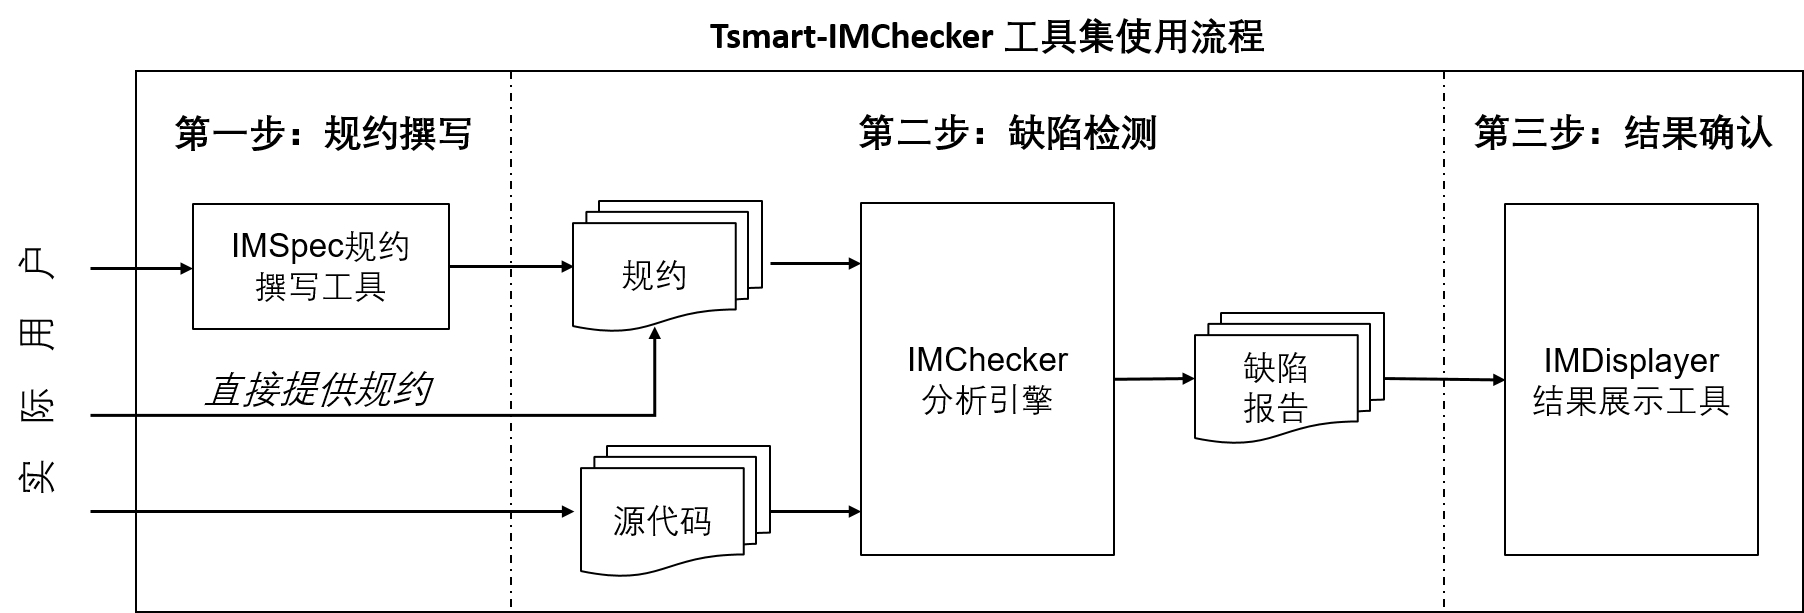
\includegraphics[width=\linewidth]{figures/cp4-overview.png}
	\caption{
		Tsmart-IMChecker工具集使用流程
	}
	\label{fig:4-3-overview}
\end{figure}

用户可以通过三个步骤使用Tsmart-IMChecker工具进行缺陷检测:
撰写规约、缺陷检测和结果确认。
首先,开发者通过IMSpec规约撰写工具,对目标接口的使用约束进行描述。
如果开发者理解IMSpec的语法结构,也可以通过直接撰写文本格式的接口使用约束条件。
在第二步,开发者通过调用缺陷检测引擎,基于提供的约束描述对源代码进行分析。
最后开发者可以直接通过生成的报告核对缺陷检测结果,
也可以通过可视化IMDisplayer工具对检测结果进行确认。
本节将在剩下的内容中对每个模块进行详细介绍。


\subsection{规约撰写模块}
接口使用约束已经被证明能够有效地应用于软件工程领域的不同任务中。
特别地,这些约束能够帮助开发者理解如何正确使用API,
以及帮助测试人员对接口误用缺陷进行检测。
然而人工撰写这些约束条件需要大量的时间与精力,
同时容易在撰写中产生错误。
为减轻使用者撰写IMSpec约束的负担、提高撰写规约语法的准确性,
本文设计并实现图形化支撑的IMSpec规约撰写工具。

如图\ref{fig:4-3-IMSpec-writer}中所示,IMSpec规约撰写工具包含三个部分:
\begin{itemize}
	\item {\kaishu 规约列表}
	界面的最左侧是规约列表,用于展示使用者已经完成的IMSpec接口约束实例。
	用户可以在列表中直观地了解已经完成的约束描述。
	目前,IMSpec撰写工具将一个复杂规约分解成多个子约束,供缺陷分析引擎使用从而提高检测精度。
	因此,显示结果为分解后的约束条件。
	\item {\kaishu 编辑区} 
	界面的右侧为规约编辑区,用于对IMSpec规约进行编辑。
	编辑区包括三大主要区域:目标对象区域、前置条件编写和后置条件编写区域。
	用户在确定目标接口的名称和参数以后,可以在下列的Ref区域选择性地填写与目标API相关的因果调用关系函数。
	例如:目标接口是\texttt{fopen()}函数,
	那么用户可以在Ref区域通过填写\texttt{fclose()}函数地定义进而强化因果调用关系。
	用户可以根据具体的接口使用约束,对前置条件和后置条件进行编辑。
	特别地,IMSpec规约撰写工具在IMSpec语法基础之上,
	在界面显示中进行细微的调整,以提供更直观、准确的功能。
	在规约撰写中,用户可以使用宏定义以保持程序语义一致性和简洁性。
	在缺陷检测阶段提供宏定义的头文件即可。
	\item {\kaishu 文件操作区} 
	界面的左下角是文件操作区域,包括加载宏定义文件、加载文件和导出三个功能。
	
\end{itemize}

\begin{figure}[t]
	\centering
	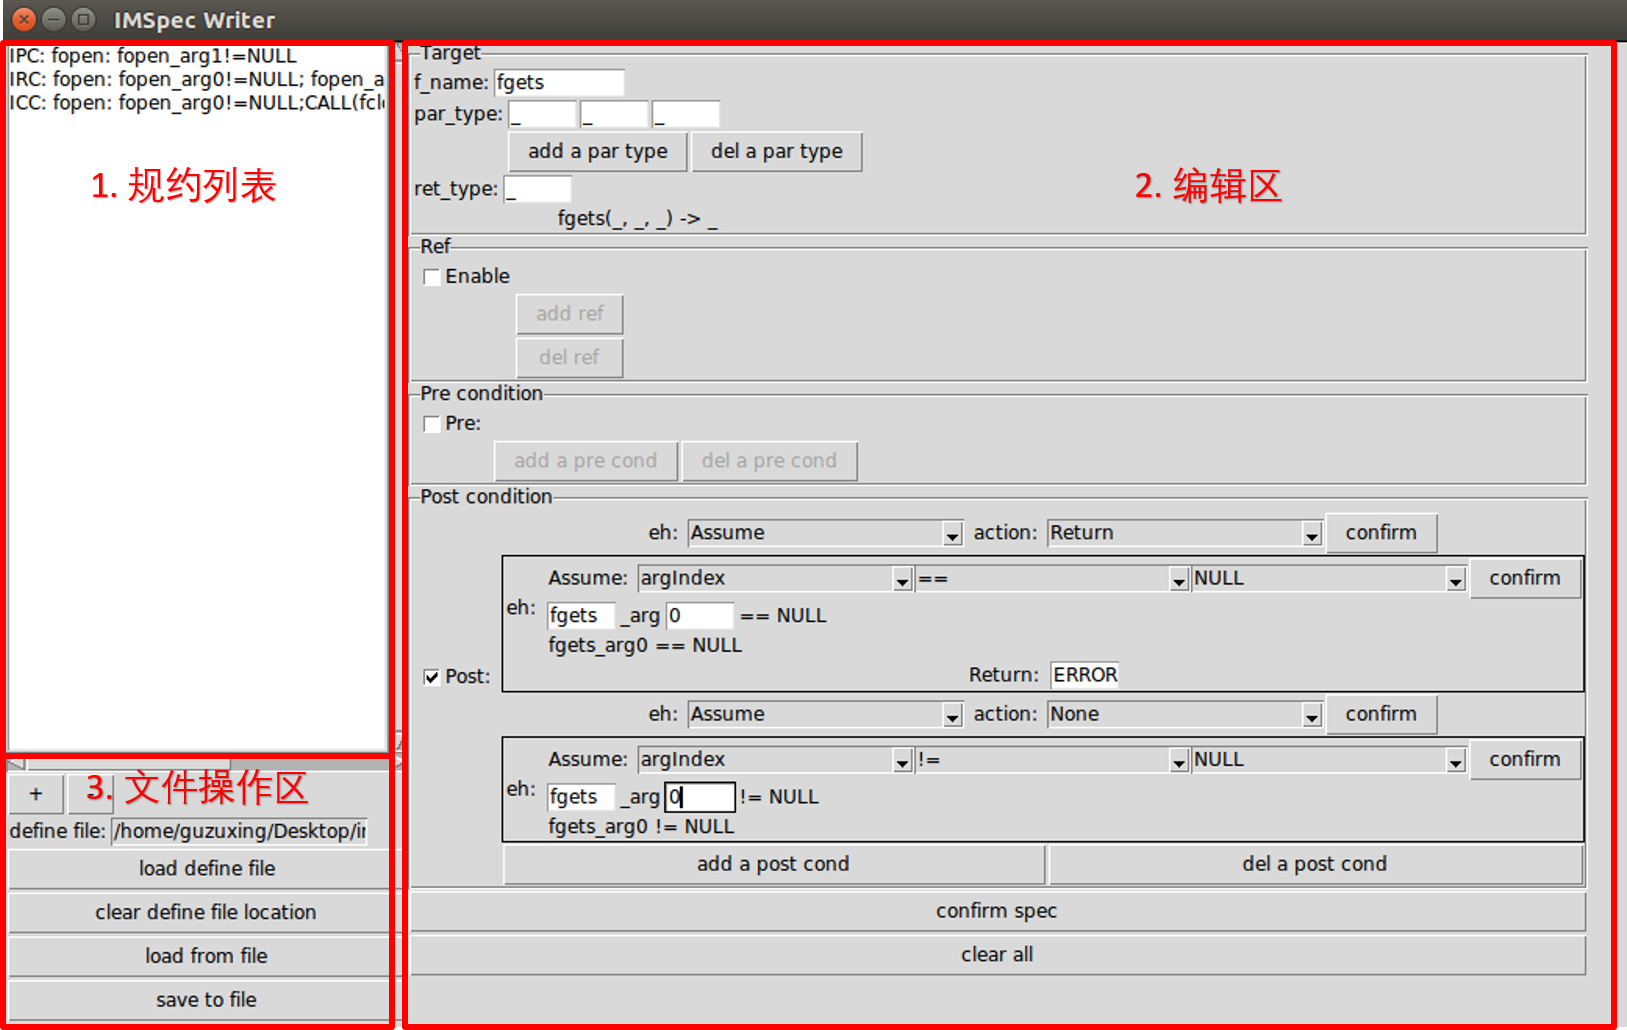
\includegraphics[width=0.85\linewidth]{figures/cp4-IMSpec-writer.png}
	\caption{
		IMSpec规约撰写工具截图
	}
	\label{fig:4-3-IMSpec-writer}
\end{figure}

用户通过命令行,执行imspec\_writer.py文件运行该工具:
\begin{lstlisting}[language={bash},
basicstyle=\linespread{0.8}\listingsfont,
numbers=none,
xleftmargin=.3\textwidth]
(*@\textcolor{blue}{Ubuntu@~:Python3}@*) imspec_writer.py
\end{lstlisting}
其运行结果被保存在用户选择目录的*.yaml文件中,
例如图\ref{fig:2-4-example-imspec}中IMSpec实例。
此外,为帮助使用者维持项目特定的语义及特殊定义,
IMSpec规约撰写工具提供了define.h文件供使用者定义宏参数。
例如,对于图\ref{fig:2-4-example-imspec}中IMSpec实例,
用户可以在define.h中定义如下宏:
\begin{lstlisting}[language={C},
basicstyle=\linespread{0.8}\listingsfont,
numbers=none,
xleftmargin=.3\textwidth]
#define SUCCESS 1
#define FILEERR -1
#define IOERR -2
\end{lstlisting}
在后续解析IMSpec语言时,解析器会进行宏定义的展开从而与程序中的语义保持一致。




\subsection{缺陷检测模块}
\begin{figure}[b]
	\centering
	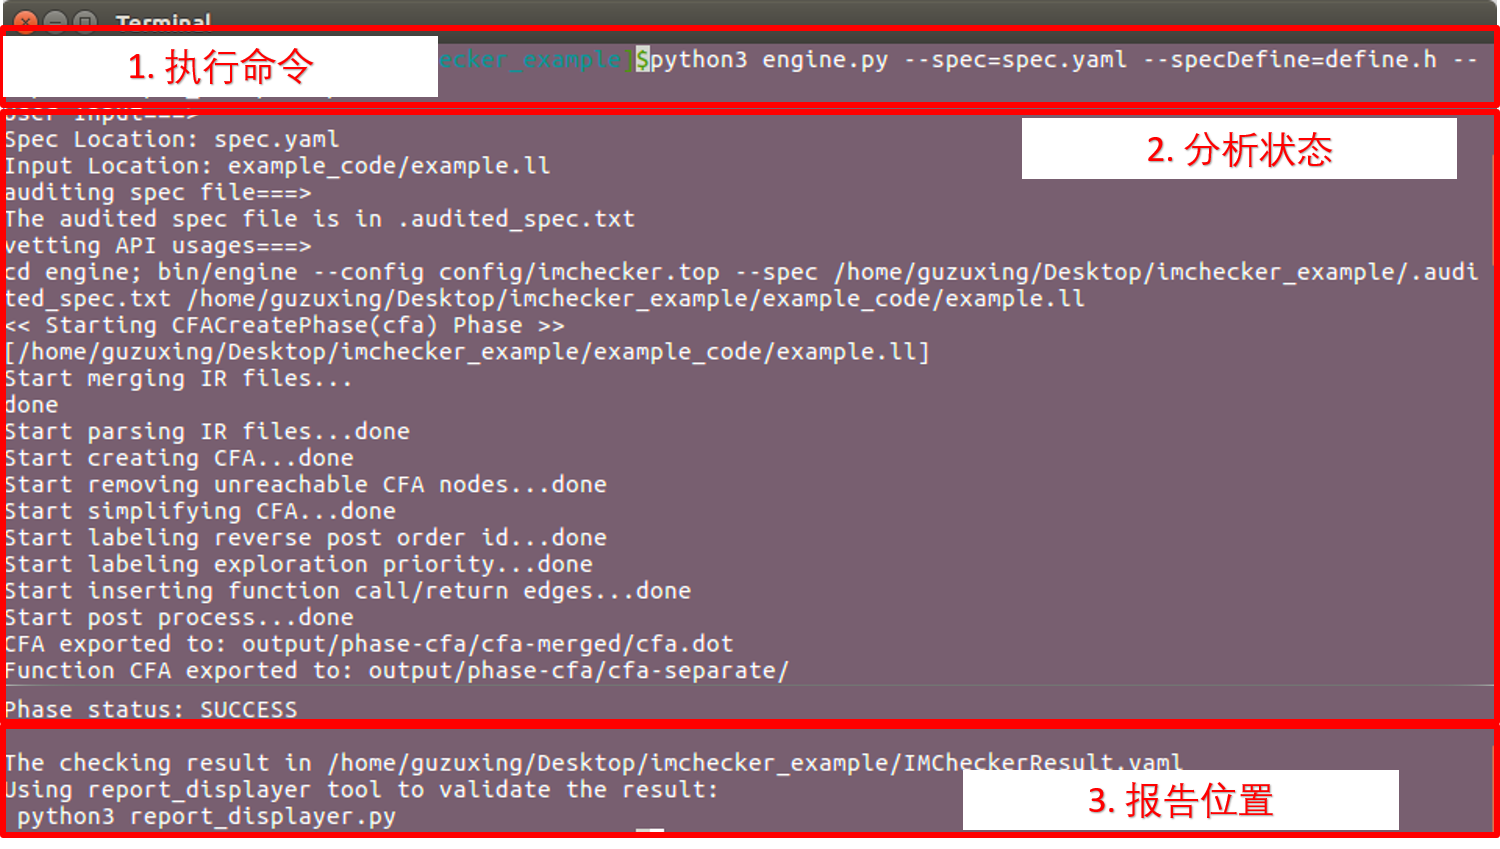
\includegraphics[width=0.85\linewidth]{figures/cp4-IMChecker-engine.png}
	\caption{
		IMChecker分析引擎运行时截图
	}
	\label{fig:4-3-IMChecker-engine}
\end{figure}

研究人员和工具开发人员通过简单易用的用户接口提高工具的实用性,减轻使用者的负担。
特别地,每个工具针对自己应用对象的不同,在工具接口上都有自己的设计目的和特点。
本文对IMChecker方法实现和封装,以命令行的方式帮助开发者直接调用分析引擎,
并生成对应的缺陷分析报告。

如图\ref{fig:4-3-IMChecker-engine}所示,IMChecker分析引擎在命令行中通过直接调用如下指令即可运行,
\begin{lstlisting}[language={bash},
basicstyle=\linespread{0.8}\listingsfont,
numbers=none,
xleftmargin=.1\textwidth]
(*@\textcolor{blue}{Ubuntu@~:Python3}@*) engine.py --spec=XXX --specDefine=XXX --input=XXX
\end{lstlisting}
其中,参数的具体含义如下:
\begin{itemize}
	\item spec: 目标接口使用约束IMSpec文件。
	该文件可以由IMSpec规约撰写工具生成,也可以用户直接根据IMSpec语法进行撰写,
	其内容如图\ref{fig:2-4-example-imspec}中IMSpec实例所示。
	\item specDefine: 规约实例中宏参数的具体定义。在分析阶段,分析引擎会根据宏定义对IMSpec规约进行展开,
	并应用于缺陷检测,
	例如在上文中介绍的define.h文件。
	\item input: 待分析文件。目前,分析引擎在单独使用时
	接受单独可编译的C程序源代码,以及预处理后的LLVM-IR中间表达。
	TsmartV3提供Build-capture编译抓取工具,
	能够自动生成LLVM-IR表达。
	使用者亦可以通过Clang对项目进行编译,通过-S指令生成LLVM-IR表达。
	如果用户通过TsmartV3工具对接口缺陷进行检测,则不需要考虑预处理操作,
	详细使用说明可以参考TsmartV3用户手册~\cite{tsmart}。
\end{itemize}

在分析过程中,IMChecker分析引擎将运行时状态输出到控制台中,以帮助开发者获得分析进展情况。
同时,对于分析中遇到的问题,开发者可以获知原因并进行修复。
如图\ref{fig:4-3-IMChecker-engine}所示,分析引擎首先对IMSpec规约文件进行解析,
接着进入预处理阶段创建CFA、分析阶段,最后针对于分析结果输出到缺陷检测结果报告IMCheckerResult.yaml中。

\begin{figure}[b]
	\centering
	\begin{minipage}{0.7\linewidth}
\begin{lstlisting}[language={C},
basicstyle=\linespread{0.7}\listingsfont,
numbers=none,frame=trBL,
xleftmargin=0pt]
  - (*@\textcolor{blue}{Bug}@*):
    (*@\textcolor{blue}{API}@*): fopen
    (*@\textcolor{blue}{Type}@*): IPC
    (*@\textcolor{blue}{Spec}@*):  fopen==> fopen_arg1!=NULL
    (*@\textcolor{blue}{Reason}@*): Missing or incorrect validation of parameter
    (*@\textcolor{blue}{Error}@*): 
      - IMChecker/tools/example_code/example.c:bad1:14
    (*@\textcolor{blue}{Good}@*): 
      - IMChecker/tools/example_code/example.c:good1:52
\end{lstlisting}
	\end{minipage}
	\caption{
		IMChecker分析结果示例
	}
	\label{fig:4-3-Result}
\end{figure}

IMChecker分析引擎将结果输出到缺陷检测报告中,针对每一个目标API的一种缺陷模式,
缺陷检测结果将汇总在一个“Bug”标签中。
图\ref{fig:4-3-Result}中给出图\ref{fig:2-4-example}中程序检测的一个缺陷实例,其中:
\begin{itemize}
	\item Bug标签为一个目标API某一种缺陷的起始标记符号。
	\item API标签给出目标API的函数名。
	\item Type标签给出缺陷的具体类型。在实际应用场景中,本文将缺陷的类型进行进一步扩展从而展示更具体的缺陷原因。
	例如,IPC表示不正确地参数使用。
	具体参数定义可以参见TsmartV3用户手册。
	\item Spec标签给出导致误用的具体约束条件。图中所描述的约束是第一个参数不可以为NULL。
	\item Reason标签给出基于自然语言的缺陷原因。目前针对于每一个缺陷类型,IMChecker提供一段自然语言描述的缺陷原因。
	\item Error标签给出具体缺陷发生的程序位置。
	\item Good标签给出针对目标API正确使用的程序位置,即满足约束的函数调用位置。
\end{itemize}
如果,该类型的错误存在多个实例或者存在多个正确的使用实例,则Error和Good标签拥有多个实例。
使用者可以通过缺陷检测结果报告对缺陷进行核对,也可以通过IMDisplayer工具进行分析。
此外,该缺陷报告也可以供其他工具的开发者利用。


\subsection{结果展示模块}
\begin{figure}[b]
	\centering
	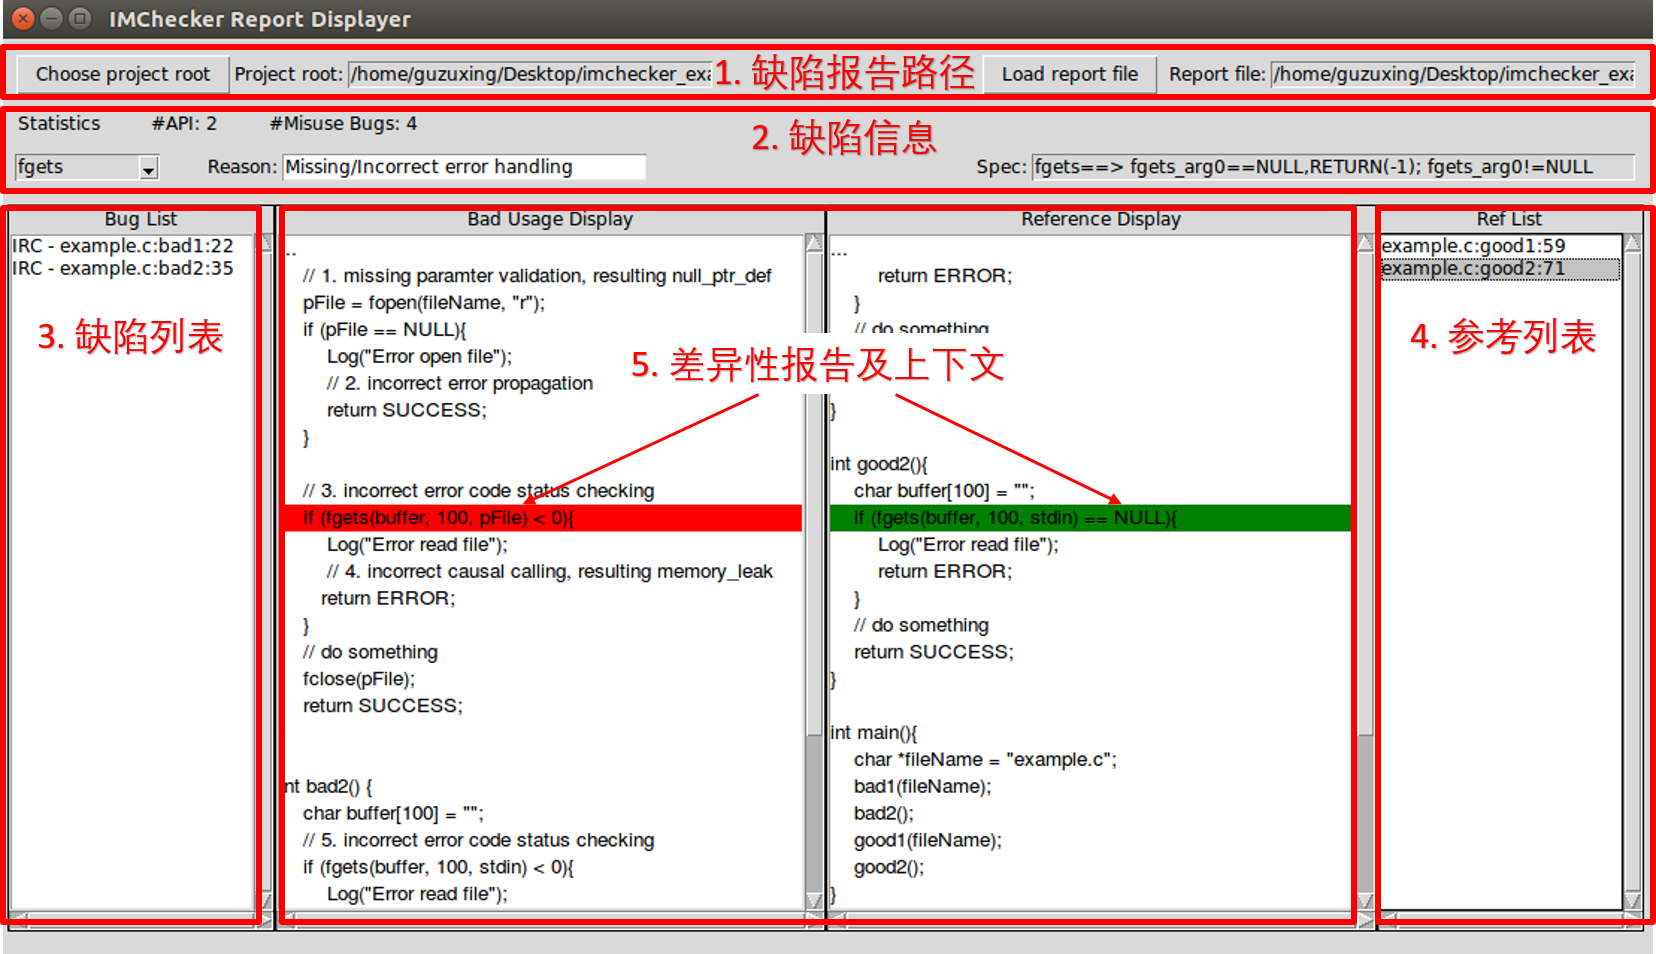
\includegraphics[width=0.85\linewidth]{figures/cp4-IMDisplayer.png}
	\caption{
		IMDisplayer结果展示工具运行时截图
	}
	\label{fig:4-3-IMDisplayer}
\end{figure}

为更好地对缺陷结果进行展示,研究人员和开发者设计并实现各种各样的GUI界面。
针对接口使用和接口误用缺陷的特点,本文设计并实现IMDisplayer结果展示工具,
通过差异性结果对比的方式,帮助开发者深入理解API使用上下文的不同,
并为开发者修复缺陷提供参考。

IMDisplayer结果展示工具在命令行中通过直接调用如下指令即可运行,
\begin{lstlisting}[language={bash},
basicstyle=\linespread{0.8}\listingsfont,
numbers=none,
xleftmargin=.3\textwidth]
(*@\textcolor{blue}{Ubuntu@~:Python3}@*) report_displayer.py
\end{lstlisting}
如图\ref{fig:4-3-IMDisplayer}所示,IMDisplayer工具包含五个部分:
缺陷报告路径选择模块、缺陷信息展示模块、缺陷列表、参考列表以及差异性报告及上下文信息。
用户在使用该工具时,首先要选择缺陷报告的路径信息。
基于缺陷报告,IMDisplayer工具会自动统计缺陷报告中的缺陷实例,
并将误用API数目、缺陷实例数目展示在界面上。
用户通过下拉菜单选择目标API。
如图中所示,目标接口为\texttt{fgets()}函数。
在用户选择目标API后,IMDisplayer工具会更新左侧的缺陷列表,以展示该接口所有误用的情况。
此后,用户可以通过点击左侧的缺陷列表选择具体要审查的缺陷实例。
在用户进行选择后,IMDisplayer会更新缺陷实例的原因、违反的约束,以及右侧参考列表。
用户可以通过对参考列表中的使用实例进行选择,
在缺陷展示框中对缺陷和正确使用进行差异性对比。
例如,图中红色和绿色为缺陷发生的位置和对应的正确使用的位置以及上下文信息。

IMDisplayer的设计动机来源于两点:
(1)IMSpec有效性评估结果显示,相对于自然语言IMSpec规约描述语言对接口使用约束描述更加有效,
即开发者更容易理解使用约束的条件。
因此,作者将缺陷具体违反的约束IMSpec形式展示在界面中,帮助开发者理解缺陷发生的原因。
(2)在应用阶段,开发者提交缺陷报告给对应的开发者。
最初只提供缺陷发生的原因和路径信息,
开发者则表示如果能提供过多的语义信息将有助于理解缺陷的原因。
因此,作者扩展缺陷分析引擎IMChecker,并设计IMDisplayer工具。
特别地,在分析过程中将正确使用的路径进行记录。
在IMDisplayer中,通过差异性比对的方式展现缺陷和正确使用代码片段。
不仅能够有效地帮助使用者理解缺陷的原因,同时能够提供缺陷修复的参考代码。
(3)IMDisplayer独立于分析引擎,通过解析缺陷报告中的标签来展示。
因此,该工具能够扩展到其他应用场景。

\section{案例应用}
\label{sec:4.4}
本文工作旨在对实际项目中C程序接口误用缺陷进行检测,以提高代码质量、应对现代软件开发的迫切需求。
因此,本章将Tsmar-IMChecker工具应用于广泛使用的开源项目中评估本文研究的有效性。
本小结将对应用对象和方法进行介绍、总结应用的结果、
并讨论实际应用中的发现和不足,
为研究人员和开发人员提供思路。

\subsection{实验准备}
\paragraph{应用对象}
本文选取三个典型领域的开源项目作为应用对象,评估Tsmar-IMChecker工具在实际项目中的有效性,
包括:操作系统Linux内核、广泛使用的第三方库OpenSSL安全库和
使用第三方库的应用软件。
其中,应用软件为Ubuntu16.04中,使用OpenSSL安全库的应用软件。
Ubuntu系统提供多个版本的OpenSSL安全库的实现,
本文采用libssl1.0.0\footnote{https://packages.ubuntu.com/xenial/libssl1.0.0}作为应用对象。

应用软件的选择步骤如下。
首先,本文通过Ubuntu系统提供的软件包依赖管理工具搜索所有使用libssl1.0.0的应用软件包,
即通过如下命令,
\begin{lstlisting}[language={bash},
basicstyle=\linespread{0.8}\listingsfont,
numbers=none,
xleftmargin=.25\textwidth]
(*@\textcolor{blue}{Ubuntu@~:}@*) apt-cache rdepends libssl1.0.0
\end{lstlisting}
\texttt{apt-cache rdepends}命令\footnote{http://manpages.ubuntu.com/manpages/bionic/man1/apt-rdepends.1.html}
能够查看一个软件包被哪些软件包所依赖。
搜索的结果显示,超过1200应用软件包依赖于libssl1.0.0。
接着,对于这些软件包本文在Github中搜索是否存在这些软件包的源代码。
目的在于找到这些应用对象中哪些仍然活跃于开源社区中,
从而提交的缺陷报告可以及时获得回复。
对于软件包进行编译、分析需要大量的时间,
因此本文共选择15个广泛使用、不同应用领域、开发者持续维护的应用软件。
为有效评估Tsmar-IMChecker的检测能力(是否能够发现未知的接口误用缺陷),所有应用对象选择截止至2018年7月10-15日的最新稳定版本,
即Linux内核4.18-rc4,OpenSSL-1.1.1-pre8,以及Ubuntu操作系统中应用软件:
\begin{itemize}
	\item dma: 邮件服务,主分支,86个关注(Star数目)
	\item exim: 邮件服务,版本4.91,393个关注
	\item hexchat: 网络实时聊天,版本2.14.1,1949个关注
	\item httping: 针对HTTP请求的Ping服务,主分支,302个关注
	\item ipmitool: 针对智能平台管理接口(Intelligent Platform Management Interface,IPMI)的控制系统,主分支,122个关注
	\item open-vm-tools: WMware软件管理,版本10.3.0,956个关注
	\item irssi: 通信软件,版本1.1.1,1918个关注
	\item keepalive: 负载均衡管理软件,版本2.0.5,1717个关注
	\item thc-ipv6: IPV6攻击测试软件,主分支,442个关注
	\item freeradius-server: 多协议服务器,主分支,943个关注
	\item trafficserver: 网络代理服务器,版本7.1.3,907个关注
	\item tinc: VPN后台服务,版本1.1-pre16,854个关注
	\item sslplit: SSL/TLS攻击测试工具,主分支,1106个关注
	\item rdesktop: 远程桌面服务,主分支,577个关注
	\item proxytunnel: 网络代理服务,主分支,155个关注
\end{itemize}

\paragraph{目标API}
目标API包括两个部分:
(1)对于Linux内核和OpenSSL,本文将第\ref{sec:2.5}节中撰写的IMSpec约束作为目标API,
旨在通过这些被误用过的API再次对这些项目进行检测,从而观察是否依旧存在误用情况。
(2)对于15个Ubuntu中的应用软件,
本文首先通过GNU cflow\footnote{http://www.gnu.org/software/cflow/}抽取这些应用软件的函数调用图。
基于函数调用图和OpenSSL提供的用户手册,选择调用图中使用OpenSSL库中的接口。
例如在dma项目中,通过cflow和OpenSSL用户手册比对的结果,
本文发现该项目使用OpenSSL中包含\texttt{SSL\_connect()}等17个不同的API。
接着在15个项目中,本文将API的使用情况进行总结,选取至少使用过三次的接口。
最终共选择78个不同的API作为检测目标。
本文将这些目标API的IMSpec规约描述文件公开\footnote{https://github.com/tomgu1991/IMChecker/tree/master/imspec},
供研究人员和开发者使用。

\begin{table}[b]
	\centering
	\begin{minipage}[t]{0.7\linewidth} % 如果想在表格中使用脚注,minipage是个不错的办法
		\caption{Tsmart-IMChecker实际项目应用结果}
		\label{tab:4-4-result}
		\begin{tabular}{cccc}
			\hline
			项目名称 & 缺陷报告总数 & 确认未修复 & 已经修复 \\
			\hline
			Linux内核 & 30 & 20 & 5 \\
			 OpenSSL & 17 & 5 & 12\\
			  dma  & 1 & 0 & 1\\
			   exim   &2  & 0 & 2\\
			    hexchat    & 2 & 1 & 0\\
			   httping & 1 & 1 & 0\\
			   ipmitool  & 1 & 1 & 0\\
			    open-vm-tools   &2  & 0 & 2\\
			     irssi    & 2 & 1 & 0\\
			 keepalive & 2 & 0 & 2\\
			 thc-ipv6 & 2 & 0 & 2\\
			 freeradius-server & 2 & 0 & 2\\
			 trafficserver & 3 & 0 & 0\\  
			  tinc  & 2 & 0 & 2\\
			   sslplit   & 2 & 0 & 2\\
			   rdesktop     & 2 & 0 & 0\\
			      proxytunnel    & 2 & 0 & 0\\
			      总计 & 75 & 29 & 32 \\
			\hline
		\end{tabular}
	\end{minipage}
\end{table}


\paragraph{实验环境}
本文在一台装有64位Ubuntu 16.04的台式机上进行实验。
该机器配有Intel(R) Core(R) i5-3470@3.20GHz-4核心CPU和32GB内存。
Tsmart-IMChecker工具需要通过Clang对项目进行预处理,抽取LLVM-IR的中间表达。
然而,部分项目无法完全被Clang支持,例如Linux内核。
同时,部分项目依赖于旧版本的编译环境或者其他编译库难以满足。
针对于这些情况,本文通过人工编译的方式,对这项目中使用目标API的文件进行单独编译,
并将这些能够编译的文件作为分析目标提供给分析引擎。
为控制分析的时间和输出结果,本文每次分析执行一个目标API。
所有的分析中,本文以3小时作为时间界限,即如果三小时无法完成,则将已有分析结果输出。
对于所有找到的实际缺陷,本文进行缺陷理解和归纳,
并在对应的项目中提交缺陷报告或者提交修改申请(Pull Request)。

\subsection{缺陷检测结果}
%https://github.com/tomgu1991/IMChecker/blob/master/evaluation_data/new_bugs/bug_list.md

如表\ref{tab:4-4-result}所示,
Tsmart-IMChecker工具针对于上述17个开源项目共检测到超过100个实际缺陷,
并对其中75个缺陷进行整理提交缺陷报告。
在第一列中,给出项目的名称;
在第二列中,对缺陷提交总数进行展示;
第三列和第四列分别给出在提交的缺陷中,开发者已经确认但没有修复的个数,
以及开发者确认并且修复的缺陷报告个数。
在所有提交的实际接口误用缺陷报告中,
Linux内核有30个,25个已经被开发者确认,其中5个已经在最新的代码中进行修复与集成。
OpenSSL共报告17个缺陷,全部被开发者确认,其中12个已经被修复并集成到主分支和发布版本中。
Ubuntu系统中的应用软件分别报告1-3个缺陷,每个项目具体数据如表中所示。
综合来看,提交的75个缺陷报告中,61个已经被开发者确认。
在确认的报告中,32个已经被成功修复。
下文将对Linux内核、OpenSSL和Ubuntu应用软件中的缺陷进行详细讨论。

\begin{table}[!b]
	\centering
	\scriptsize
	\setlength{\tabcolsep}{4.25pt}
	\begin{minipage}[t]{0.97\linewidth} % 如果想在表格中使用脚注,minipage是个不错的办法
		\caption{Linux内核-4.18rc4缺陷检测结果}
		\scriptsize
		\label{tab:4-4-linux}
		\begin{tabular}{ccclcc}
			\hline
			\multirow{2}{*}{编号}& 缺陷 & \multirow{2}{*}{误用API} & \multicolumn{1}{c}{文件位置} & 缺陷 & \multirow{2}{*}{状态\footnote{$\checkmark\checkmark$为已经修复的缺陷,$\checkmark$为确认的缺陷,$P$为未确认的缺陷。}} \\
			& 编号 & & \multicolumn{1}{c}{文件名:调用函数} & 种类 & \\
			\hline
1 & 200489 & kzalloc & tlb\_uv.c: \textbf{init\_per\_cpu} & ICC & \checkmark \\
2 & 200505 & alloc\_disk & pktcdvd.c: \textbf{pkt\_setup\_dev}& IEH & \checkmark\checkmark \\
3 & 200511& kzalloc & clk-pxa.c: \textbf{clk\_pxa\_cken\_init} & ICC & \checkmark \\
4 & 200519& devm\_clk\_get & hci\_bcm.c: \textbf{bcm\_get\_resources} & IPU & \checkmark \\
5 & 200521& kzalloc & ip22-gio.c: \textbf{ip22\_check\_gio} & ICC & \checkmark \\
6 & 200533& nla\_nest\_start & ncsi-netlink.c: \textbf{ncsi*\_nl}& IPU & \checkmark\checkmark \\
7 & 200535 & nla\_nest\_start & conntrack.c: \textbf{ovs*\_get}& IPU & \checkmark\checkmark \\
8 & 200537 & nla\_nest\_start & datapath.c: \textbf{queue*\_packet} & IPU & \checkmark \\
9 & 200539 & alloc\_skb & chtls\_cm.c: \textbf{chtls*\_conn} & ICC & \checkmark \\
10 & 200541 & \_\_send*alloc\_skb & team.c: \textbf{team\_*\_get} & ICC & \checkmark \\
11 & 200543 & devm\_kzalloc & gpio-tegra.c: \textbf{tegra\_gpio\_probe}& IEH & \checkmark \\
12 & 200545 & devm\_kzalloc & core.c: \textbf{rsnd\_probe}& IEH & \checkmark \\
13 & 200547 & devm\_kzalloc & atmel*\_output.c: \textbf{atmel\_*\_endpoint} & ICC & $P$ \\
14 & 200549 & pci*ext\_capability & nic\_main.c: \textbf{pci*\_capability} & IPU & \checkmark \\
15 & 200551 & pci*ext\_capability & dpc.c: \textbf{dpc\_probe} & IPU & \checkmark\checkmark \\
16 & 200555 & devm*init\_i2c & hmc5843\_i2c.c: \textbf{hmc5843*\_probe} & IPU & \checkmark \\
17 & 200557 & devm\_ioremap & pata\_pxa.c: \textbf{pxa\_ata\_probe} & IEH & \checkmark \\
18 & 200559 & alloc\_workqueue & fm10k\_main.c: \textbf{fm10k*\_module} & ICC & \checkmark \\
19 & 200561 & ida\_pre\_get & namespace.c: \textbf{mnt*\_id} & IPU & \checkmark\checkmark \\
20 & 200563 & wm831x*\_read & clk-wm831x.c: \textbf{wm831x*prepared} & IEH & \checkmark \\
21 & 200565 & dma\_mapping\_error & qib\_sdma.c: \textbf{qib*send} & IEH & \checkmark \\
22 & 200567 & get\_zeroed\_page & sysinfo.c: \textbf{sysinfo\_show} & IEH & \checkmark \\
23 & 200569 & kzalloc & mach-mx27ads.c: \textbf{mx27ads*\_init} & ICC & $P$ \\
24 & 200571 & kzalloc & board-v7.c: \textbf{i2c\_quirk} & ICC & \checkmark \\
25 & 200573 & kzalloc & coherency.c: \textbf{armada\_*\_init} & ICC & \checkmark \\
26 & 200575 & kzalloc & octeon-irq.c: \textbf{octeon*\_map} & ICC & \checkmark \\
27 & 200577 & kzalloc & gptu.c: \textbf{clkdev*\_gptu} & ICC & $P$ \\
28 & 200579& kzalloc & octeon-irq.c: \textbf{octeon*\_map} & ICC & $P$ \\
29 & 200581 & kzalloc & sysctrl.c: \textbf{clkdev\_add\_pci} & ICC  & $P$ \\
30 & 200583 & kzalloc & msi-xlp.c: \textbf{xlp*\_irqs} & ICC & \checkmark \\
			\hline
		\end{tabular}
	\end{minipage}
\end{table}

\paragraph{Linux内核}
如表\ref{tab:4-4-linux}中所示,在Linux内核中
Tsmart-IMChecker工具共提交30个未被报告的接口缺陷。
针对于每一个缺陷报告,本者首先在Linux的缺陷报告系统\footnote{https://bugzilla.kernel.org}中进行查询,
是否已经有相关缺陷报告。
如果没有,则对缺陷报告进行提交。
在提交报告给开发者后,其中25个已经被开发者确认并收到开发者回复的邮件。
至今,5个已经被维护者接受。
其中2个已经集成到Linux最新版当中,3个在进行代码风格修改。

\begin{figure}[b]
	\centering
	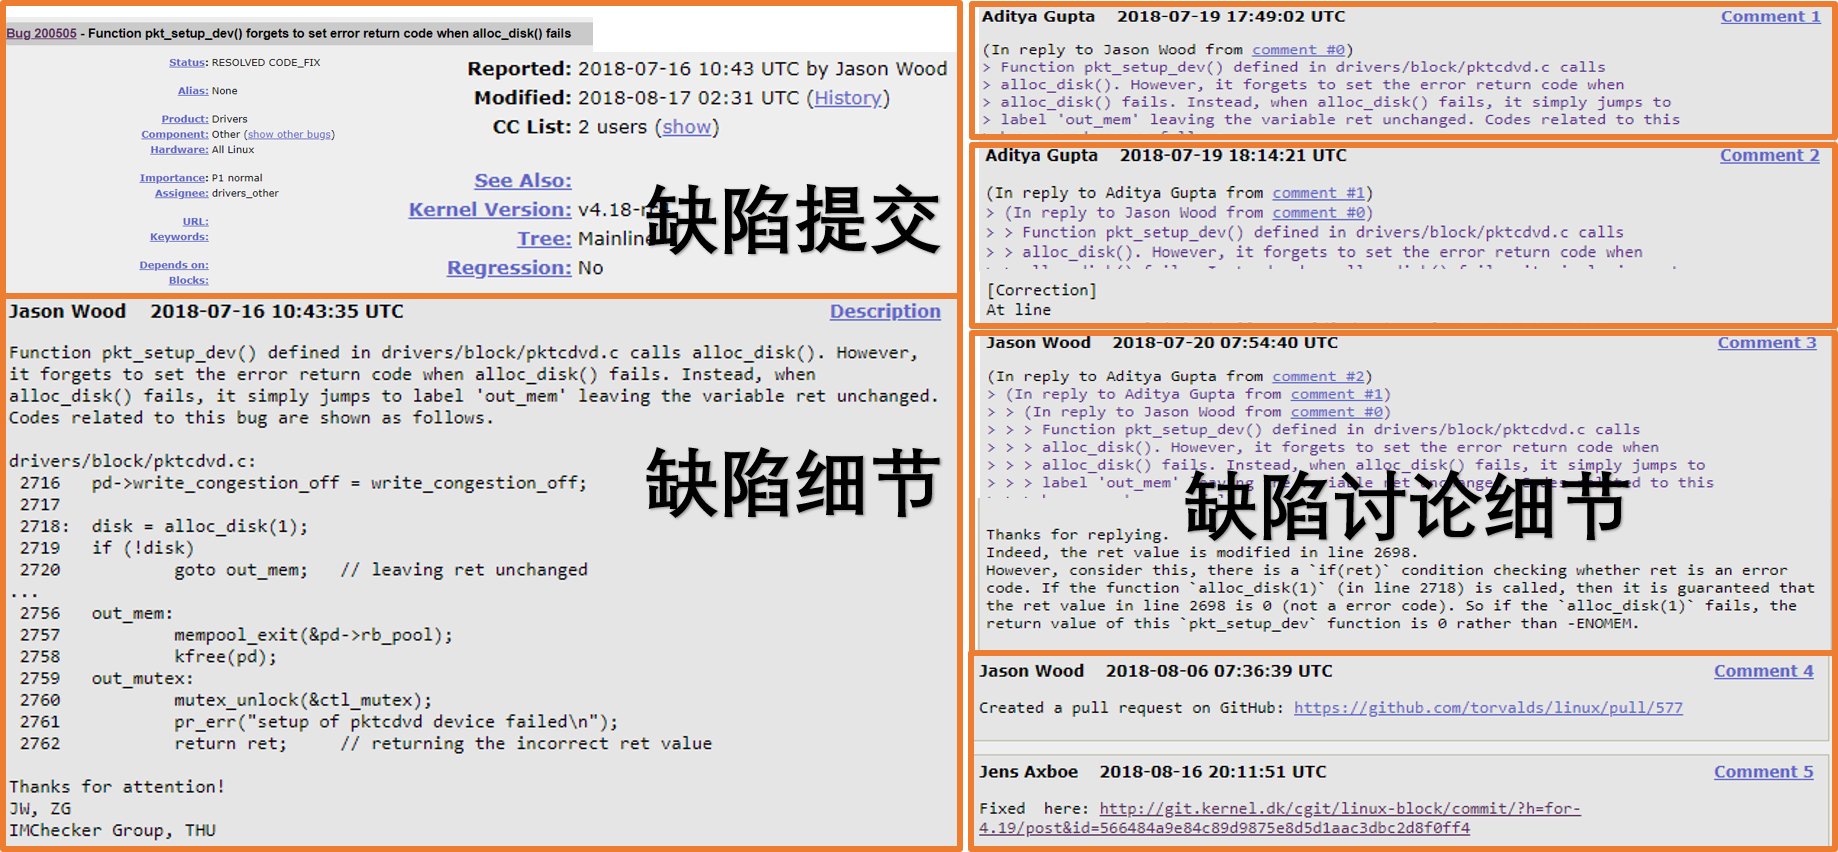
\includegraphics[width=\linewidth]{figures/cp4-linux-example.png}
	\caption{
		Linux接口误用缺陷200505提交和讨论记录
	}
	\label{fig:4-4-linux-example}
\end{figure}

\begin{figure}[t]
	\centering
	\begin{lstlisting}
(*@\textcolor{black}{"summary": "fix setting of 'ret' error return for a few cases",}@*)
"date": "2018-08-16",
"author": "Jens Axboe",
drivers/block/pktcdvd.c
=======================================================
@@ -2740,6 +2740,7 @@ static int pkt_setup_dev(dev_t dev, dev_t* pkt_dev)
pd->write_congestion_on  = write_congestion_on;
pd->write_congestion_off = write_congestion_off;

+	ret = -ENOMEM;
	disk = alloc_disk(1);
	if (!disk)
		goto out_mem;
	\end{lstlisting}
	\caption{
		Linux接口缺陷200505修复细节。
	}
	\label{fig:4-4-linux-example-fix}
\end{figure}


图\ref{fig:4-4-linux-example}为作者将误用接口\texttt{alloc\_disk()}的缺陷实例细节提交以及修复的记录截图。
根据Linux中错误处理机制,接口\texttt{alloc\_disk()}出错时,
外层调用者需要返回\textbf{-ENOMEM}来表示内存不足的错误信息。
然而在drivers/block/pktcdvd.c文件的\texttt{pkt\_setup\_dev()}函数中2718行调用该接口后,
在异常处理路径上并有对返回值进行修改,导致一个不正确的异常处理缺陷(IEH)。
在对该缺陷进行仔细核对后,本文将缺陷提交到Linux缺陷报告系统中,编号为200505。
该缺陷报告在提交后,获得维护者的回复。
在经过三轮的缺陷细节讨论过后,该缺陷被维护者确认,并修改和集成到Linux内核的主分支中。
缺陷修复的细节如图\ref{fig:4-4-linux-example-fix}中所示,
即在返回之前对返回值赋值为错误代码\textbf{-ENOMEM}。


\paragraph{OpenSSL}
\begin{table}[!b]
	\centering
	\scriptsize
	\setlength{\tabcolsep}{4.25pt}
	\begin{minipage}[t]{0.97\linewidth} % 如果想在表格中使用脚注,minipage是个不错的办法
		\caption{OpenSSL-1.1.1-pre8缺陷检测结果}
		\scriptsize
		\label{tab:4-4-openssl}
		\begin{tabular}{ccclcc}
			\hline
			\multirow{2}{*}{编号}& 缺陷 & \multirow{2}{*}{误用API} & \multicolumn{1}{c}{文件位置} & 缺陷 & \multirow{2}{*}{状态\footnote{$\checkmark\checkmark$为已经修复的缺陷,$\checkmark$为确认的缺陷。}} \\
			& 编号 & & \multicolumn{1}{c}{文件名:调用函数} & 种类 & \\
			\hline
1 & 6567 & RAND\_bytes & speed.c: \textbf{RAND*\_loop} & IEH & \checkmark\checkmark \\
2 & 6568 & ASN1\_INTEGER\_get & tasn\_utl.c: \textbf{asn1\_do\_adb} & IPU & \checkmark \\
3 & 6569& ASN1\_INTEGER\_set & p12\_init.c: \textbf{PK*init} & IPU & \checkmark\checkmark \\
4 & 6570& ASN1\_object\_size & asn1\_gen.c: \textbf{generate\_v3 } & IEH & \checkmark \\
5 & 6572& BN\_set\_word & t1\_lib.c: \textbf{ssl*\_dh} & IEH & \checkmark\checkmark \\
6 & 6573& HMAC\_Init\_ex & apps/speed.c: \textbf{HMAC\_loop} & IEH & \checkmark \\
7 & 6574 & EVP\_PKEY\_get0\_DH & statem\_srvr.c: \textbf{tls*\_dhe} & IPU & \checkmark\checkmark \\
8 & 6575 & EC\_KEY\_generate\_key & speed.c: \textbf{run\_benchmark} & IEH & \checkmark \\
9 & 6781 & EC*new*\_name & ec\_ameth.c: \textbf{eckey\_type2param} & ICC & \checkmark\checkmark \\
10 & 6789 & ASN1\_INTEGER\_set & v3\_tlsf.c: \textbf{v2i*FEATURE} & IEH & \checkmark\checkmark \\
11 & 6820 & ASN1\_INTEGER\_to\_BN & ts\_lib.c: \textbf{TS*\_bio} & IPU & \checkmark\checkmark \\
12 & 6822 & BN\_sub & rsa\_ossl.c: \textbf{rsa*\_encrypt} & IEH & \checkmark\checkmark \\
13 & 6973 & EVP\_MD\_CTX\_new & ocsp\_srv.c: \textbf{OCSP*\_sign} & IPU & \checkmark\checkmark \\
14 & 6977 & ASN1\_INTEGER\_set & pk7\_lib.c: \textbf{PKCS7*type} & IEH & \checkmark\checkmark \\
15 & 6982 & OBJ\_nid2obj & asn\_moid.c: \textbf{do\_create} & IEH & \checkmark\checkmark \\
16 & 6983 & BN\_sub & bn\_x931p.c: \textbf{BN*\_Xpq} & IEH & \checkmark\checkmark \\
17 & 7235 & DH\_set0\_key & dh\_lib.c: \textbf{DH*\_key} & IEH & \checkmark \\
			\hline
		\end{tabular}
	\end{minipage}
\end{table}

\begin{figure}[t]
	\centering
	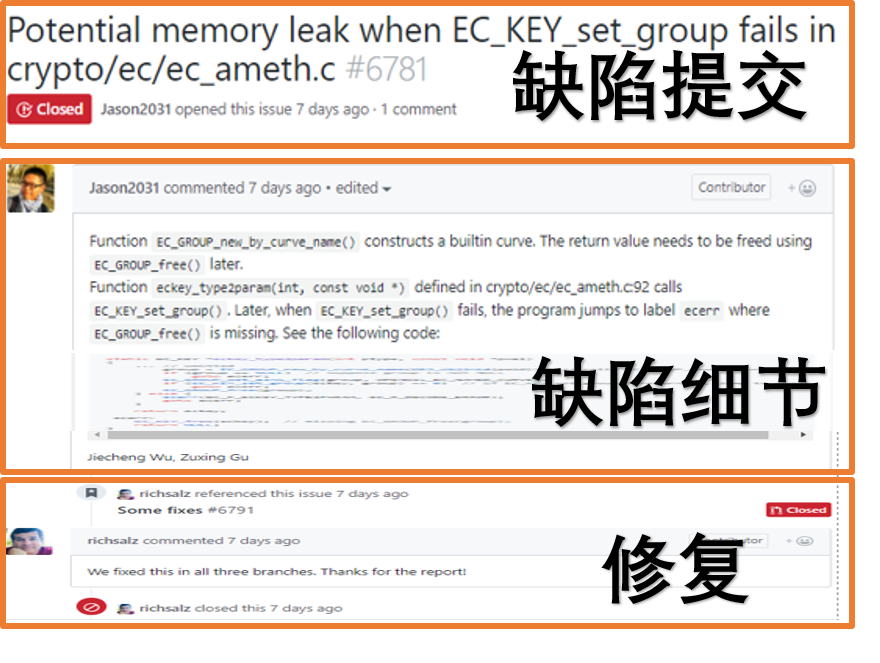
\includegraphics[width=0.8\linewidth]{figures/cp4-openssl-example.png}
	\caption{
		OpenSSL缺陷6781提交和修复记录
	}
	\label{fig:4-4-openssl-example}
\end{figure}



如表\ref{tab:4-4-openssl}中所示,在OpenSSL中Tsmart-IMChecker工具共提交17个未被报告的接口缺陷。
针对于每一个缺陷报告,本文首先在Github中OpenSSL代码库中提交Issue。
在提交报告给开发者后,所有的缺陷报告都获得开发者的回复。
其中12个已经被维护者修复并集成在主分支内,5个被标记为待评估(Assessed)。
OpenSSL与Linux内核的缺陷报告系统不同通过Github的Issue系统维护,
因此缺陷的提交和修复能够获得及时的反馈。

\begin{figure}[t]
	\centering
	\begin{lstlisting}
(*@\textcolor{black}{"summary": "Avoid memory leak on failure path.Thanks to Jiecheng Wu, Zuxing Gu for the report.",}@*)
"date": "2018-07-26",
"author": "richsalz",
=======================================================
@@ -122,13 +122,12 @@ static TLS_FEATURE *v2i_TLS_FEATURE(const X509V3_EXT_METHOD *method,
+   EC_GROUP *group = NULL;
	[...]
	else if (ptype == V_ASN1_OBJECT) {
		const ASN1_OBJECT *poid = pval;
-		EC_GROUP *group;
		[...]
		group = EC_GROUP_new_by_curve_name(OBJ_obj2nid(poid));
		if (group == NULL)
			goto ecerr;
		EC_GROUP_set_asn1_flag(group, OPENSSL_EC_NAMED_CURVE);
		if (EC_KEY_set_group(eckey, group) == 0)
			goto ecerr;
		EC_GROUP_free(group);
	} else {
	[...]
ecerr:
	EC_KEY_free(eckey);
+	EC_GROUP_free(group);
	return NULL;
	\end{lstlisting}
	\caption{
		OpenSSL缺陷6781修复细节
	}
	\label{fig:4-4-openssl-example-fix}
\end{figure}

图\ref{fig:4-4-openssl-example}是作者在OpenSSL项目检测到的一个内存泄漏缺陷。
OpenSSL设计接口\texttt{EC\_GROUP\_new\_by\_curve\_name()}来创建EC\_GROUP对象。
该对象在生命周期结束后需要通过\texttt{EC\_GROUP\_free()}进行释放。
然而在ec\_ameth.c文件的\texttt{eckey\_type2param()}的函数体内,
在一条异常处理路径上开发者并没有进行释放导致一个内存泄漏错误。
如图\ref{fig:4-4-openssl-example-fix}中所示,
开发者在12行进行内存对象的申请,
然而在16行的if判断错误处理中直接通过goto语句跳转到21行继续执行。
因此这条异常处理路径上,忽视了对于12行申请内存对象\texttt{group}的释放。
在作者提交缺陷报告并说明出错路径后,开发者在12小时内完成修复。
修复细节如图\ref{fig:4-4-openssl-example-fix}所示。

OpenSSL项目设计明确的错误代码机制,并在用户手册中提供基于自然语言的描述。
然而,项目的开发者却忽略大量的异常处理检测。
例如,缺陷6572、6789和6982,均由不正确的异常处理原因导致的软件缺陷。
作者在提交缺陷报告后,开发者均进行相应的修复。




\paragraph{应用程序}

\begin{table}[!t]
	\centering
	\setlength{\tabcolsep}{2.25pt}
	\begin{minipage}[t]{\linewidth} % 如果想在表格中使用脚注,minipage是个不错的办法
		\caption{Ubuntu16.04应用软件缺陷检测结果}
		\label{tab:4-4-apps}
		\begin{tabular}{ccclcc}
			\hline
			 项目 & 缺陷 & \multirow{2}{*}{误用API} & \multicolumn{1}{c}{文件位置} & 缺陷 & \multirow{2}{*}{状态\footnote{$\checkmark\checkmark$为已经修复的缺陷,$\checkmark$为确认的缺陷,$P$为未确认的缺陷。}} \\
			名称 & 编号 & & \multicolumn{1}{c}{文件名:调用函数} & 种类 & \\
			\hline
dma & 59 & SSL\_connect & crypto.c: \textbf{smtp*\_crypto} & IEH & \checkmark\checkmark \\
\cline{1-1}
\multirow{2}{*}{exim} & 2316 & X509\_NAME\_oneline & tls-openssl.c: \textbf{x509*\_names} & IEH & \checkmark\checkmark \\
    & 2317 & SSL\_CTX*\_list & tls-openssl.c: \textbf{tls*\_cb} & IEH & \checkmark\checkmark \\
\cline{1-1}
\multirow{2}{*}{hexchat} & 2244 & BN\_set\_word & dh1080.c: \textbf{dh1080\_init} & IEH & \checkmark \\
    & 2245 & DH\_set0\_key & dh1080.c: \textbf{dh1080\_compute\_key} & IEH & $P$ \\
\cline{1-1}
\multirow{1}{*}{httping} & 41 & SSL\_CTX\_new & mssl.c: \textbf{initialize\_ctx} & ICC & \checkmark \\
\cline{1-1}
\multirow{1}{*}{ipmitool} & 37 & MD2\_Init & auth.c: \textbf{ipmi\_auth\_md2} & IEH & \checkmark \\
\cline{1-1}
\multirow{1}{*}{open-} & 291 & SSL\_*list & sslDirect.c: \textbf{SSL\_NewContext} & IEH & \checkmark\checkmark \\
vm-tools & 292 & X509*\_current\_cert & certverify.c: \textbf{VerifyCallback} & IPU & \checkmark\checkmark \\
\cline{1-1}
\multirow{2}{*}{irssi} & 943 & SSL*\_certificate & net*-openssl.c: \textbf{irssi*\_handshake} & IPU & $P$ \\
    & 944 & BIO\_read & certverify.c: \textbf{set*\_info} & IEH & \checkmark \\
\cline{1-1}
\multirow{2}{*}{keepalive} & 1003 & SSL*\_new & ssl.c: \textbf{build*\_ctx} & ICC & \checkmark\checkmark \\
    & 1004 & SSL\_new & ssl.c: \textbf{ssl\_connect} & ICC & \checkmark\checkmark \\
\cline{1-1}
\multirow{2}{*}{thc-ipv6} & 28 & BN\_new & thc-ipv6-lib.c: \textbf{thc\_memstr} & ICC & \checkmark\checkmark \\
    & 29 & BN\_set\_word & thc-ipv6-lib.c: \textbf{thc\_memstr} & IEH & \checkmark\checkmark \\
\cline{1-1}
\multirow{2}{*}{FreeRADIUS} & 2309 & BIO\_new & session.c: \textbf{tls*\_cert} & ICC & \checkmark\checkmark \\
    & 2310 & i2a\_ASN1\_OBJECT & session.c: \textbf{tls*\_cert} & IEH & \checkmark\checkmark \\
\cline{1-1}
\multirow{3}{*}{trafficserver} & 4292 & SSL\_CTX\_new & http\_load.c: \textbf{handle\_connect} & ICC & $P$ \\
    & 4293 & SSL\_new & http\_load.c: \textbf{handle\_connect} & ICC & $P$ \\
    & 4294 & SSL\_write & http\_load.c: \textbf{handle\_connect} & IEH & $P$ \\
\cline{1-1}
\multirow{2}{*}{tinc} & 205 & BN\_hex2bn & tincd.c: \textbf{keygen} & IPU & \checkmark\checkmark \\
    & 206 & RAND\_load\_file & tincd.c: \textbf{main} & IEH & \checkmark\checkmark \\
\cline{1-1}
\multirow{2}{*}{sslsplit} & 224 & SSL*\_certificate & pxyconn.c: \textbf{pxy*\_create} & IEH & \checkmark\checkmark \\
    & 225 & SSL*\_PrivateKey & pxyconn.c: \textbf{pxy*\_create} & IEH & \checkmark\checkmark \\
\cline{1-1}
\multirow{2}{*}{rdesktop} & 280 & BN\_bin2bn& ssl.c: \textbf{rdssl*\_encrypt} & IEH & $P$ \\
    & 281 & BN\_mod\_exp & ssl.c: \textbf{rdssl*\_encrypt} & IEH & $P$ \\
\cline{1-1}
\multirow{2}{*}{proxytunnel} & 36 & SSL\_connect & ptstream.c: \textbf{stream*\_ssl} & IEH & $P$ \\
    & 37 & SSL\_new& ptstream.c: \textbf{stream*\_ssl} & ICC & $P$ \\
			\hline
		\end{tabular}
	\end{minipage}
\end{table}

OpenSSL软件库是网络通信领域广泛使用的安全库,这些接口误用会极大地损害系统的可靠性。
因此,对OpenSSL项目中接口缺陷检测本身具有重要意义。
一方面,可以提高软件库本身的质量;
另一方面,通过完善软件库代码的质量,能够有效地为使用者提供可靠的使用样例。

我们在Ubuntu16.04的应用软件中,对OpenSSL软件库接口缺陷进行检查。
检测结果显式,这些应用软件存在大量的接口误用缺陷。
本文在对结果分析、核对和整理后,
将28检测结果提交到对应的15个项目中。
如表\ref{tab:4-4-apps}所示,28个缺陷中19个被开发者接受,其中15个已经被成功修复。
特别地,dma、exim、open-vm-tools、keepalive、thc-ipv6、FreeRADIUS、tinc和sslplit八个项目,对缺陷报告进行及时的确认和修复。
虽然其他项目对缺陷报告没有修复,但部分报告已经被开发者确认并标记为下一个版本需要处理的问题。
其他报告则处于没有回复的阶段,即开发者并没有否定检测结果为误报。
同时,相应的缺陷模式已经在其他的项目中获得认可。
因此,本文认为这些缺陷具有极高的可信度。

\begin{figure}[t]
	\centering
	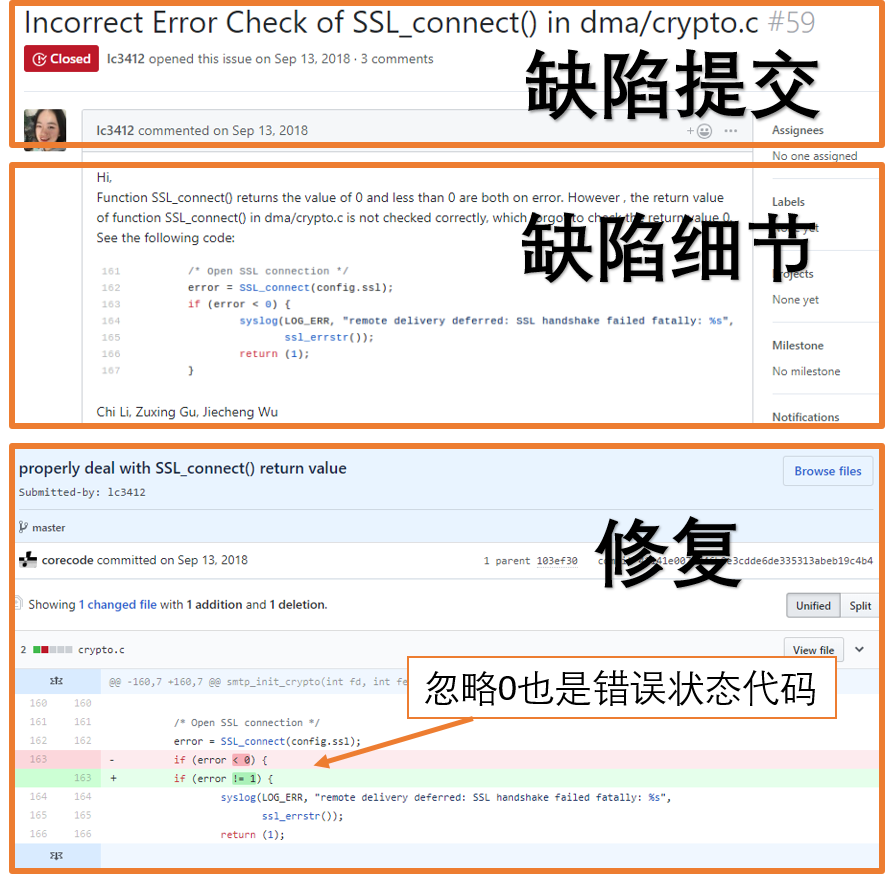
\includegraphics[width=0.8\linewidth]{figures/cp4-dma-example.png}
	\caption{
		dma缺陷59提交和修复记录
	}
	\label{fig:4-4-dma-example}
\end{figure}

图\ref{fig:4-4-dma-example}是本文在dma项目检测到的一个不正确的异常处理错误。
OpenSSL的官方用户手册中指出,接口\texttt{SSL\_connect()}用于初始化TSL/SSL服务器握手操作(handshake)。
根据TSL/SSL协议本身,当握手失败时该函数的实现返回0代表链接被成功关闭,返回负数则代表错误发生在协议层、链接等等。
因此,该接口的错误状态代码有两种情况,针对该函数的异常处理也需要考虑这两种情况。
如图中代码所示,在dma项目中开发者只对负数进行检查,而忽略错误状态代码为0的情况。
因此,当\texttt{SSL\_connect()}函数在执行时返回0时,该项目的异常处理机制将失效,程序的鲁棒性将会被破坏。
dma项目为邮件服务,因此该错误极大可能被攻击者利用从而产生漏洞。
本文在提交缺陷报告后,开发者进行了即使修复。
如图中所示,开发者对错误状态代码的判断进行完善,从而正确执行异常处理机制。



\subsection{应用经验总结}
本文将Tsmart-IMChecker应用于实际开源项目中,
对接口缺陷进行分析并将缺陷报告提交给相应的开发者。
本文将缺陷检测、报告提交、开发者讨论和后续跟进工作中
遇到的困难、发现和项目应用经验总结在下文中。
主要包括如下几个方面:
接口误用缺陷、现有文档、缺陷提交和开发者态度。

\paragraph{接口误用缺陷}
同第\ref{sec:2.3}节调研结果一致,接口误用缺陷并不是个例,普遍存在于各种软件系统中。
特别地,本文共找到超过100个实际缺陷,并提交75个缺陷报告给实际开发者。
其中61个(81.33\%)被开发者接受,32个(42.67\%)已经被开发者修复。
在本文分析之前Linux内核和OpenSSL软件库作为广泛使用的基础软件,
两者代码已经被著名的分析工具(例如,商业工具Coverity~\cite{coverity}和学术工具Clang Static Analysis)检测过。
更严重的是这些缺陷的目标API均从已有的缺陷修改记录中获得,
即这些缺陷已经在过去发生过。
同时,被分析的应用软件中每个都至少误用一个OpenSSL的接口。
%我们在后续的研究中,在其他的应用软件中发现同样的现象。
在对缺陷模式、细节分析后,本文发现这些缺陷产生存在两方面的原因:
(1)软件库开发者间缺少缺陷报告分享机制。
开发者经常会忘记接口使用的约束。
特别地,即使新的代码中存在和过去发生的缺陷的模式一样,
并没有一个能够自动检测的方法,对开发者进行提示。
(2)客户端开发者缺少足够的领域知识,导致误用库函数,
即客户端开发者在使用OpenSSL软件库时,没有深入理解或者参考文档,
导致接口使用错误。

总结来说,开发者在开发过程中难免会产生接口误用,无论是无意忘记约束,还是本身缺少理解。
因此,规模化、高效的分析工具对接口误用缺陷检测具有重要的实际意义。
特别地,Tsmart-IMChecker基于规约描述语言进行检测,
集成大量的领域知识并容易扩展。
同时可以渐进式分析,即可以只应用于新修改的代码中。

\begin{figure}[b]
	\centering
	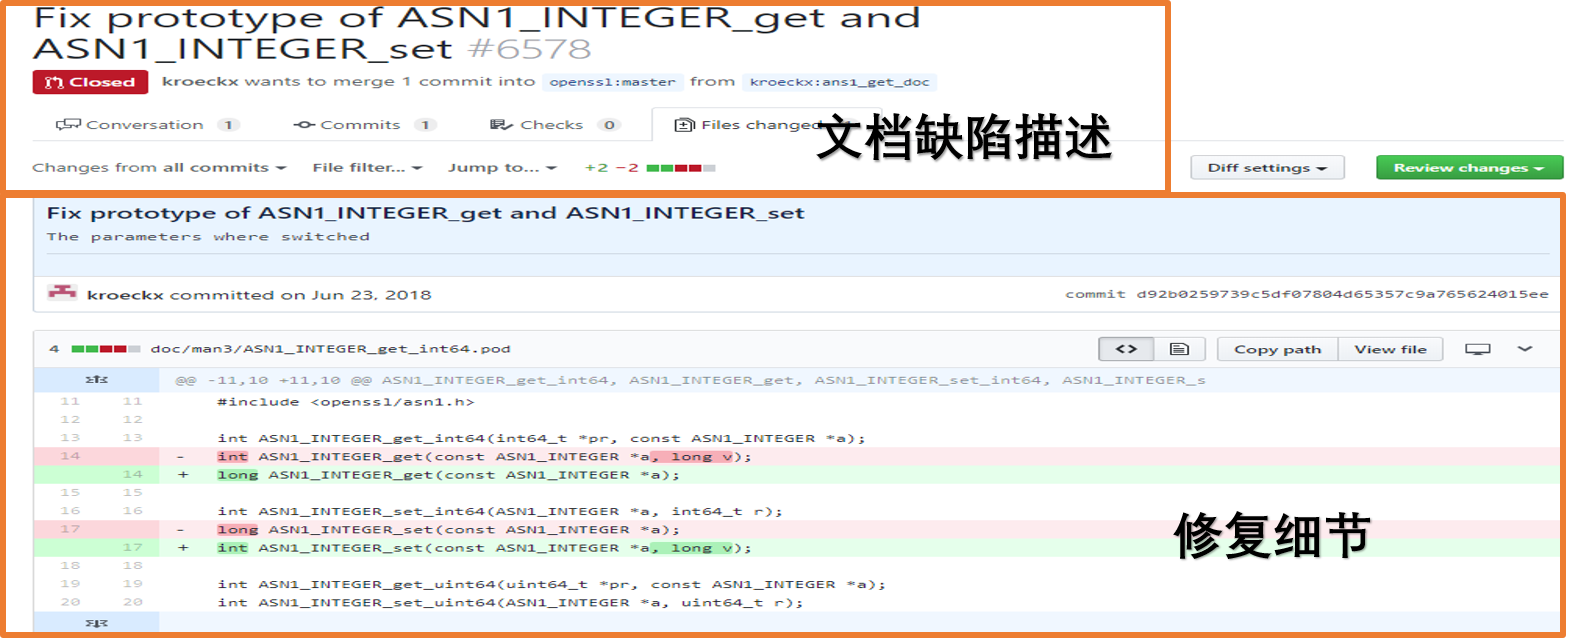
\includegraphics[width=\linewidth]{figures/cp4-doc-bug.png}
	\caption{
		OpenSSL中接口用户手册缺陷修复记录
	}
	\label{fig:4-4-doc-bug}
\end{figure}
\begin{figure}[t]
	\centering
	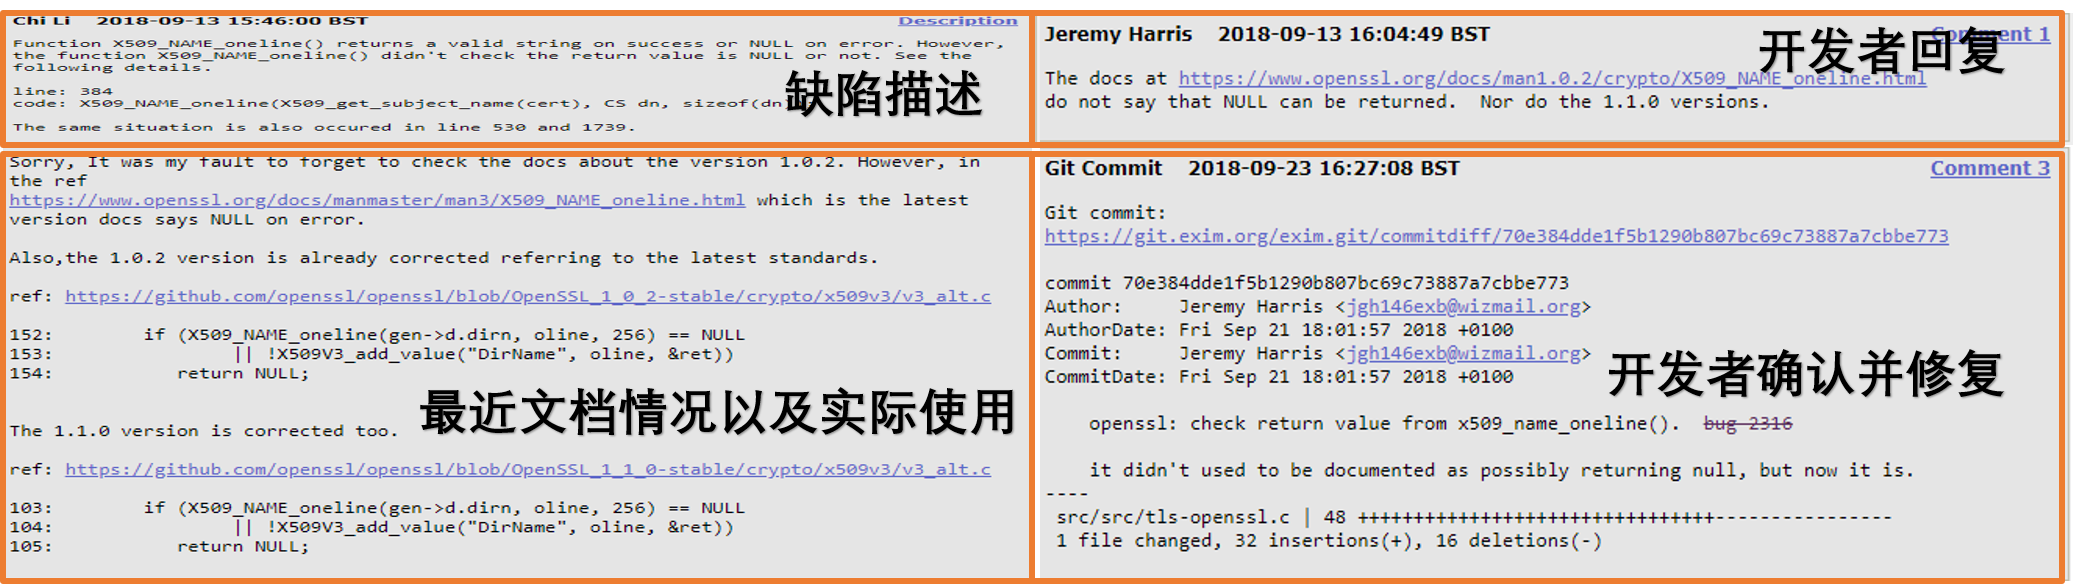
\includegraphics[width=\linewidth]{figures/cp4-exim-bug.png}
	\caption{
		exim项目中缺陷2316修复记录
	}
	\label{fig:4-4-exim-bug}
\end{figure}
\paragraph{现有文档}
虽然OpenSSL软件库为使用者提供格式优良的自然语言描述的接口使用约束和解释,
然而在本文分析的15个应用软件中,依旧存在大量的接口误用缺陷。
对缺陷报告和文档进行分析后,现有的文档存在如下几个不足:
\begin{itemize}
	\item 文档自身存在错误。在OpenSSL的缺陷检测中,本文发现OpenSSL提供的官方文档中存在错误。
	在进行代码具体使用情况和文档描述的核对后,本文提交文档和接口缺陷报告(Issue-6569)。
	开发者在收到缺陷报告后,1天内对文档进行修复,如图\ref{fig:4-4-doc-bug}中所示。
	\item 文档利用率不足。一方面,软件库的代码实现中本身存在对库接口的误用;
	另一方面,客户端开发者对文档参考不足,误用这些接口。
	在和开发者讨论接口误用原因时,超过一半的开发者表示
	在遇到使用问题时更喜欢去Google或者Stack-overflow中搜索,
	而不是参考官方文档。
	\item 客户端未能感知软件库的更新。
	如图\ref{fig:4-4-exim-bug}中所示,在exim项目中作者在提交缺陷报告(ID-2316\footnote{https://bugs.exim.org/show\_bug.cgi?id=2316})后,
	开发者根据旧版本的用户手册认为缺陷不成立。
	然而,在OpenSSL最新的用户手册和最新的代码中,已经对相应的接口进行更新。
	在提交相应的说明后,开发者对缺陷修复。
\end{itemize}

总结来说,即使现有的软件库提供格式良好的使用说明和参考用例,
开发者在遇到问题时,依旧首选网络平台进行咨询。
然而,根据调研结果显示~\cite{18-icse-stack},网络平台中的代码质量并不可靠。
特别地,随着开源软件社区的蓬勃发展,大量的软件库缺少文档。
所以,现有的文档形式难以满足用户的需求。
因此,本文基于缺陷模式设计面向C程序接口使用约束的领域特定语言IMSpec。
该语言旨在和现有的自然语言描述形成互补,以提供更好的接口使用约束描述方法。



\paragraph{缺陷提交}
在缺陷检测后,本文针对于选择的缺陷实例细节进行深入分析,并提交缺陷报告给相应的开发者。
起初,在缺陷报告中只包含错误的位置和原因。
开发者很少反馈,或者希望作者提供更多的有效信息。
在此基础之上,作者丰富缺陷报告,
即在报告中包含:缺陷位置、原因、具体路径信息和对比正确使用片段,
供开发者更好地理解缺陷。
对于改进后的缺陷报告,提交的多数报告被开发者接受并修复。
作者将缺陷报告提交中的经验总结如下:
\begin{itemize}
	\item 开发者更喜欢提交代码修复(Pull Request)。
	在缺陷提交的过程中,Linux内核的维护者表示只接受修复提交。
	同样,Ubuntu的应用软件的开发者则更欢迎提交修复代码。
	OpenSSL开发者欢迎提交修复代码,同时积极地在帮助作者进行缺陷修复。
	\item 提交策略。
	在缺陷报告提交初期,本文连续地提交数十个缺陷报告,
	获得回复较少。
	一个可能的原因为开发者认为这样的缺陷报告是批量产生,质量不高。
	此后,作者降低提交频率,不仅获得较多回复,同时缺陷的认可和修复率都提高。
	\item 缺陷报告信息要充分。
	如上文所述,丰富缺陷报告信息,能够有效地帮助开发者理解缺陷细节。特别是缺陷产生的上下文,以及如何正确使用目标接口。
\end{itemize}

总结来说,缺陷提交需要大量的人力进行信息核对和确认。
在提交过程中,作者发现开发者更喜欢接受修复代码。
然而,缺陷修复需要大量的领域知识和上下文信息。
此外,基于差异性的路径信息能够有效地帮助开发者理解缺陷原因,并提供可能的缺陷修复模式。
因此,在Tsmart-IMChecker工具集中本文设计并实现基于差异性对比的缺陷结果展示工具IMDisplayer。

\begin{figure}[b]
	\centering
	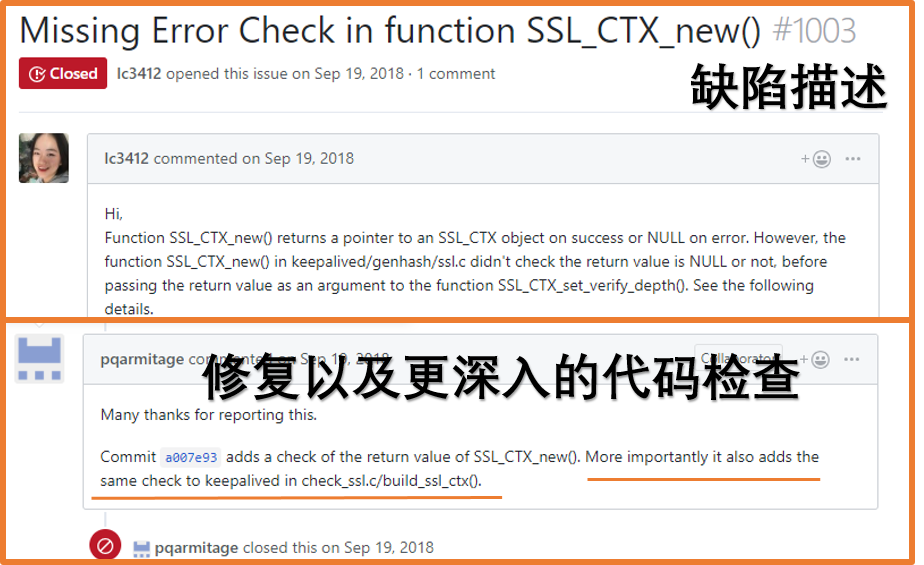
\includegraphics[width=0.8\linewidth]{figures/cp4-keepalived-fix.png}
	\caption{
		keepalived开发者根据本文缺陷报告进行深入的代码检查
	}
	\label{fig:4-4-keepalived-fix}
\end{figure}

\paragraph{开发者态度}
在缺陷报告的过程中,开发者展现出不同的态度。
一方面,开发者对缺陷报告进行积极响应,例如OpenSSL的开发者多数在1天就完成缺陷的修复。
另一方面,开发者则更希望作者提供实际的运行轨迹或者提供修复代码,而不仅仅是缺陷报告。
本文将与开发者的交流和讨论中总结出的特殊发现描述如下,
\begin{itemize}
	\item 开发者自身忽视接口使用的约束。
	在实际开发过程中,开发者难以做到完全正确。
	即使是简单的参数检查和返回值检查,在大量的代码中普遍存在这种缺陷。
	然而,这些缺陷难以通过人工的方式进行一一排查。
	特别地,当开发者认识到这些缺陷时,会对其他代码中同样的缺陷模式进行检测。
	如图\ref{fig:4-4-keepalived-fix}所示,在keepalived项目中,
	本文提交缺陷报告后,开发者不仅修复对应的缺陷,还对其他的代码进行类似缺陷的检测和修复。
	\item 特殊目的。
	虽然有些接口确实被误用,但是开发者故意为之或者在特殊的应用内无需修复。
	例如OpenSSL项目提供app/speed.c文件用于测试算法速度。
	因此在代码中,存在大量的缺少必要返回值检查的接口误用(IssueID-6575)。
	OpenSSL一个开发者认为这些误用在这个上下文中并不需要关注。
	然而,其他开发者认为这部分代码作为应用中的案例,是其他开发者的重要参考需要重视。
	开发者进行深入的讨论后,决定在后续的开发过程中进行统一处理(Assessed)。
	另一方面,由于C程序缺少异常处理机制,开发者会故意忽略部分异常检测,
	因为软件设计时本身就没有考虑这些情况。
\end{itemize}

总结来说,基于有效信息的缺陷报告能够获得开发者积极的反馈。
同时并不是所有的接口误用都会引起开发者的关注,
特别地有一些误用是开发者故意为之。
例如,提高运行效率、C程序无法支持的异常处理情况和接口本身的特殊性等等。


\section{本章小结}
\label{sec:4.5}
本章将C程序接口使用约束领域特定语言IMSpec和规模化接口误用缺陷检测方法IMChecker在实际项目中进行应用。
为帮助研究人员和开发者理解接口误用缺陷,本文整理C程序接口误用缺陷数据集APIMU4C。
该数据集包含来源于实际项目的接口误用案例库以及接口误用测试数据集,
从而帮助研究人员和开发者对检测工具的性能进行评估、针对性选择检测工具以及设计设计新的检测算法。
同时,本章设计并实现可视化支撑的C程序接口误用缺陷检测工具集Tsmart-IMChecker,
并将工具集应用于开源项目缺陷检测中。
应用结果显示,本文的方法能够有效地检测到实际项目中的未被发现的接口误用缺陷,并
在Linux内核、OpenSSL库和Ubuntu系统应用软件的最新稳定版本中提交75个实际缺陷报告。
其中62个已经被开发者确认,32个被开发者修复。
\chapter{结束语}
\label{cha:con}

\section{工作总结}
本文针对C程序接口缺陷的检测问题,从接口使用规约描述、缺陷检测算法和实际项目应用三个角度展开系统性研究,取得相应理论成果、实现相应的工具集合。本文的工作具体总结如下:
\begin{enumerate}
	\item 提出基于缺陷模式的接口使用规约描领域特定语言IMSpec。
	为理解C程序接口缺陷特性,本文对六个不同领域被广泛使用的开源软件中830个接口误用缺陷修复报告进行研究,总结出三大类通用接口缺陷模式(参数、异常处理和函数调用关系)。
	基于缺陷模式特性,本文提出接口使用特定相关的规约描述语言IMSpec,并给出IMSpec语言的设计思路、语法结构与形式化语义。
	IMSpec能够有效的描述实际项目中接口误用实例的接口使用约束,为形式化定义接口使用约束条件与接口缺陷检测打下基础。
	
	\item 设计基于接口使用约束的规模化接口缺陷检测引擎IMChecker-engine。
	该引擎通过对目标接口的使用情况进行计算,构造分析上下文环境。通过多入口分析策略将大规模代码静态分析任务分解为独立的子任务。
	针对每一个子任务,即一个目标接口的某个特定调用上下文,通过提取和目标接口缺陷相关的程序语句,并利用抽象符号对路径的语义信息进行记录。
	最后基于目标接口的使用约束对抽象路径上进行缺陷检测。
	对于多入口分析带来的精度损失,本文通过基于上下文的语义信息以及基于使用情况的统计信息两种策略对检测结果进行过滤与排序。
	本文在公开数据集Juliet Test Suite的13个接口缺陷相关的CWE分类上取得了13.21\%的误报率和16.80\%的漏报率。
	该结果领先于主流的开源静态分析工具。
	
	\item 开发C程序接口缺陷检测工具集Tsmart-IMChecker。
	该工具集包含可视化规约撰写工具IMSpec-write、缺陷分析引擎IMChecker-engine以及基于差异性对比的结果展示工具IMDisplayer。
	本文将Tsmart-IMChecker工具集应用于开源项目中,在最新的Linux内核、OpenSSL安全协议加密库以及Ubuntu操作系中应用软件中找到75个新的接口误用缺陷,并提交缺陷报告给相应的开发者。
	其中61个已经被开发者确认,32个被开发者修复。
	本文将实际项目应用中的结果和经验进行总结。
	同时,基于接口缺陷实例,本文构造了C程序接口误用数据集APIMU4C,以帮助研究人员和开发者更好的理解C程序接口缺陷、评估检测工具的能力以及展开新的研究工作。
	
\end{enumerate}


\section{研究展望}
在现有的研究基础上,为进一步保障C程序接口的正确使用,拟从如下3 个方面开展进一步的研究:
\begin{enumerate}
	\item 目前IMSpec规约描述语言由人工撰写。虽然IMSpec提供了轻量级的语法形式以及IMSpec-writer可视化撰写工具,人工撰写规约依旧需要一定工作量。特别是针对于没有文档的接口以及缺少领域经验的开发者,接口使用规约的正确性难以保证。
	自动规约挖掘技术能够从大量的代码库中学习接口使用规约。
	因此可以集成现有基于数据挖掘技术的规约推理工具,以利用自动化学习的结果。
	目前,IMSpec能够有效的支持现有挖掘技术的规约模式。
	一个可能的工作流程可以是,首先利用自动挖掘技术对规约进行学习并生成规约列表,供用户选择和修改。
	针对缺失的规约,用户可以直接撰写相应的约束条件。
	此外,一个可靠的规约分享平台能够有效的在不同开发者间分享已有规约描述。
	
	\item 为了支持大规模代码缺陷检测,本文采取了基于多入口的分析策略。
	因此分析中引入上下文信息丢失带来的精度损失。
	可能解决方案包括:
	(1)增加跨函数的摘要信息计算,以获得更加准确的上下文信息,提升过滤效果;
	(2)设计基于概率模型的排序算法,以优先展示具有高置信度、高影响域的缺陷检测结果;
	(3)设计基于缺陷模式的领域特定路径提取策略,以优化、针对性的获取更加丰富的语义信息。
	
	
	\item 研究自动化接口缺陷修复技术,以辅助开发者修复缺陷。
	本文在对接口缺陷检测的过程中,记录正确的使用路径以帮助开发者理解缺陷原因、提供缺陷修改意见。
	后续,可以结合代码综合技术,自动化生成修复补丁,降低开发者的维护成本。
	另一方面,针对修复后的代码,可以采用回归分析的策略,降低代码分析成本。
	特别地,对已经检测过得目标接口,如果对应的上下文情况没有修改,则不必进行缺陷检测。
\end{enumerate}
%(18P161)



%%% 其它部分
\backmatter

%% 本科生要这几个索引,研究生不要。选择性留下。
% 插图索引
%\listoffigures
% 表格索引
%\listoftables
% 公式索引
%\listofequations


%% 参考文献
% 注意:至少需要引用一篇参考文献,否则下面两行可能引起编译错误。
% 如果不需要参考文献,请将下面两行删除或注释掉。
% 数字式引用
\bibliographystyle{thuthesis-numeric}
% 作者-年份式引用
% \bibliographystyle{thuthesis-author-year}
\bibliography{ref/refs}


%% 致谢
% 如果使用声明扫描页,将可选参数指定为扫描后的 PDF 文件名,例如:
% \begin{acknowledgement}[scan-statement.pdf]
\begin{acknowledgement}
  首先衷心感谢导师顾明老师和孙家广老师对本人精心的指导。
  依旧记得在本科保研的时候,顾老师对我提出的要求和希望,
  是我一辈子的目标。
  在五年的博士生活中每当遇到困难和疑惑时,
  与顾老师的讨论总能帮我找到可行的解决方案。
  特别感谢顾老师肯定我的能力,支持我的研究工作,并提供给我全方面的帮助。
  孙老师是我最敬仰的老师之一,
  他严谨、勤奋、谦卑的工作态度让我终生受益。
  难以忘记每天早上和孙老师在实验室讨论工作,
  给我分享成功的秘诀、深刻的软件工程思想。
  特别感谢孙老师派我到美国交换,让我开阔视野。

  
  在美国伊利诺伊斯大学厄巴纳香槟分校进行六个月的交换学习期间,
  承蒙Lui Sha教授热心指导与Andrew Ou热心帮助,不胜感激。
  初到美国,感谢Andrew帮助我解决日常生活中的困难,
  带我领略异国他乡的风采,品尝当地美食。
  在研究期间,感谢Lui教授教我如何快速学习领域知识、
  如何与非计算机专业人士进行有效沟通,
  以及为我介绍领域专家帮我开拓研究领域。
  

  感谢实验室的老师和师兄一直以来对我的指导和照顾。
  感谢周旻老师带领我们静态分析小组。
  感谢姜宇老师,帮我分析我的研究内容、指导我的论文写作,
  在平时督催我、在困难时给我鼓励。
  感谢刘浛和刘嘉祥两位师兄教我如何做学术报告、帮我修改论文、给我鼓励和信心。
  感谢张华枫师兄在我入组以来,在生活中对我无微不至的关怀,并指出我的不足。  
  感谢吴捷成和李池,无条件信任我的决策,加入到我的博士论文工作当中。
  特别感谢我的博士同窗于庆涵,在我住院时对我的照顾,平日里一起吃饭、讨论、相互鼓励,
  愿我们的友谊地久天长。
  
  
  感谢我的女友刘畅。我们2007年高中相识,至今已经12年。
  六年的恋爱时间里,我们从异地到异国再到异地。
  感谢你一直以来对我的理解和关怀,陪我一起坚守这份感情。
  在我情绪低落时为我鼓励加油,在我骄傲满足时提醒我。
  你最美丽的年华陪我度过,我必不辜负于你。
  
  最后感谢我的父母。你们的包容、支持和关爱是我顺利走过博士求学之路最大保障。
  我们每年只有过年的10天能够团聚,平日里你们也担心打扰我的工作,
  每次回家我总能感受到家的温馨与快乐。
  父母对我的为人处世的教导以及社会经验的传授让我受益匪浅。
  
  本课题承蒙多项国家基金的支持,特此致谢。
\end{acknowledgement}


%% 附录
%\begin{appendix}
%\chapter{外文资料原文}
\label{cha:engorg}

\title{The title of the English paper}

\textbf{Abstract:} As one of the most widely used techniques in operations
research, \emph{ mathematical programming} is defined as a means of maximizing a
quantity known as \emph{bjective function}, subject to a set of constraints
represented by equations and inequalities. Some known subtopics of mathematical
programming are linear programming, nonlinear programming, multiobjective
programming, goal programming, dynamic programming, and multilevel
programming$^{[1]}$.

It is impossible to cover in a single chapter every concept of mathematical
programming. This chapter introduces only the basic concepts and techniques of
mathematical programming such that readers gain an understanding of them
throughout the book$^{[2,3]}$.


\section{Single-Objective Programming}
The general form of single-objective programming (SOP) is written
as follows,


%\end{appendix}

%% 个人简历
\begin{resume}

  \resumeitem{个人简历}

  1991 年 06 月 02 日出生于 辽宁 省 大连 市。

  2010 年 9 月考入 南开 大学 软件学院  软件工程 专业,2014 年 7 月本科毕业并获得 工学 学士学位。

  2014 年 9 月免试进入 清华 大学 软件 学院攻读 博士 学位至今。

  \researchitem{发表的学术论文} % 发表的和录用的合在一起

  % 1. 已经刊载的学术论文(本人是第一作者,或者导师为第一作者本人是第二作者)
  \begin{publications}
    %\item Yang Y, Ren T L, Zhang L T, et al. Miniature microphone with silicon-
    %  based ferroelectric thin films. Integrated Ferroelectrics, 2003,
    %  52:229-235. (SCI 收录, 检索号:758FZ.)
    \item \textbf{Gu Z}, Jiang Y, et al. A Cyber-Physical System Framework for Early Detection of Paroxysmal Diseases[J]. IEEE Access, 2018, 6: 34834-34845. (SCI 收录, 检索号:GN6RX,影响因子4.199)
    \item Wang Y, \textbf{Gu Z}, et al. A constraint-pattern based method for reachability determination[C]//Proceedings of the 41st IEEE Annual Computer Software and Application Conference, Turin, Italy, 2017: 85-90. (CCF-C 类会议,EI 检索号:20174304306998)
    \item \textbf{Gu Z}, Song H, et al. An integrated Medical CPS for early detection of paroxysmal sympathetic hyperactivity[C]//2016 IEEE International Conference on Bioinformatics and Biomedicine (BIBM), Shenzhen, China, 2016, pp. 818-822. (CCF-B 类会议,EI 检索号:20170803377769)
  \end{publications}

  % 2. 尚未刊载,但已经接到正式录用函的学术论文(本人为第一作者,或者
  %    导师为第一作者本人是第二作者)。
  \begin{publications}[before=\publicationskip,after=\publicationskip]
    %\item Yang Y, Ren T L, Zhu Y P, et al. PMUTs for handwriting recognition. In
    %  press. (已被 Integrated Ferroelectrics 录用. SCI 源刊.)
    \item \textbf{Gu Z}, Wu J C, et al. Vetting API Usages in C Programs with IMChecker. In press. (已被41th International Conference on Software Engineering录用,CCF-A 类会议)
    \item \textbf{Gu Z}, Zhou M, et al. IMSpec: An Extensible Approach to Exploring the Incorrect Usage of APIs. In press. (已被13th International Symposium on Theoretical Aspects of Software Engineering录用,CCF-C 类会议)
    \item \textbf{Gu Z}, Wu J C, et al. An Empirical Study on API-Misuse Bugs in Open-Source C Programs. In press. (已被 43rd IEEE Annual Computer Software and Application Conference录用,CCF-C 类会议)
    \item \textbf{Gu Z}, Wu J C, et al. SSLDoc: Automatically Diagnosing Incorrect SSL API Usages in C Programs. In press. (已被 The 31st International Conference on Software Engineering \& Knowledge Engineering录用,CCF-C 类会议)
    \item Li Chi, Zhou Min, \textbf{Gu Z}, et al. VBSAC: A Value-Based Static Analyzer for C. In press. (已被 28th ACM SIGSOFT International Symposium on Software Testing and Analysis录用,CCF-A 类会议)
  \end{publications}


  \researchitem{参与的科研项目}
  \begin{achievements}
  	\item 2016.4-2016.12:国家自然科学基金重大集成项目“可信嵌入式软件系统试验环境与示范应用”(No.91218302)
  	\item 2016.9 至今:科技部国家重点研发计划“规模化漏洞分析与应用关键技术研究”(No.2016QY07X1402)
  	
  	
  \end{achievements}

  \researchitem{研究成果} % 有就写,没有就删除
  \begin{achievements}
    %\item 任天令, 杨轶, 朱一平, 等. 硅基铁电微声学传感器畴极化区域控制和电极连接的
    %  方法: 中国, CN1602118A. (中国专利公开号)
    \item TsmartV3工具集:http://tsmart.tech
    \item APIMU4C数据集:https://github.com/imchecker/compsac19
  \end{achievements}

\end{resume}


%% 本科生进行格式审查是需要下面这个表格,答辩可能不需要。选择性留下。
% 综合论文训练记录表
%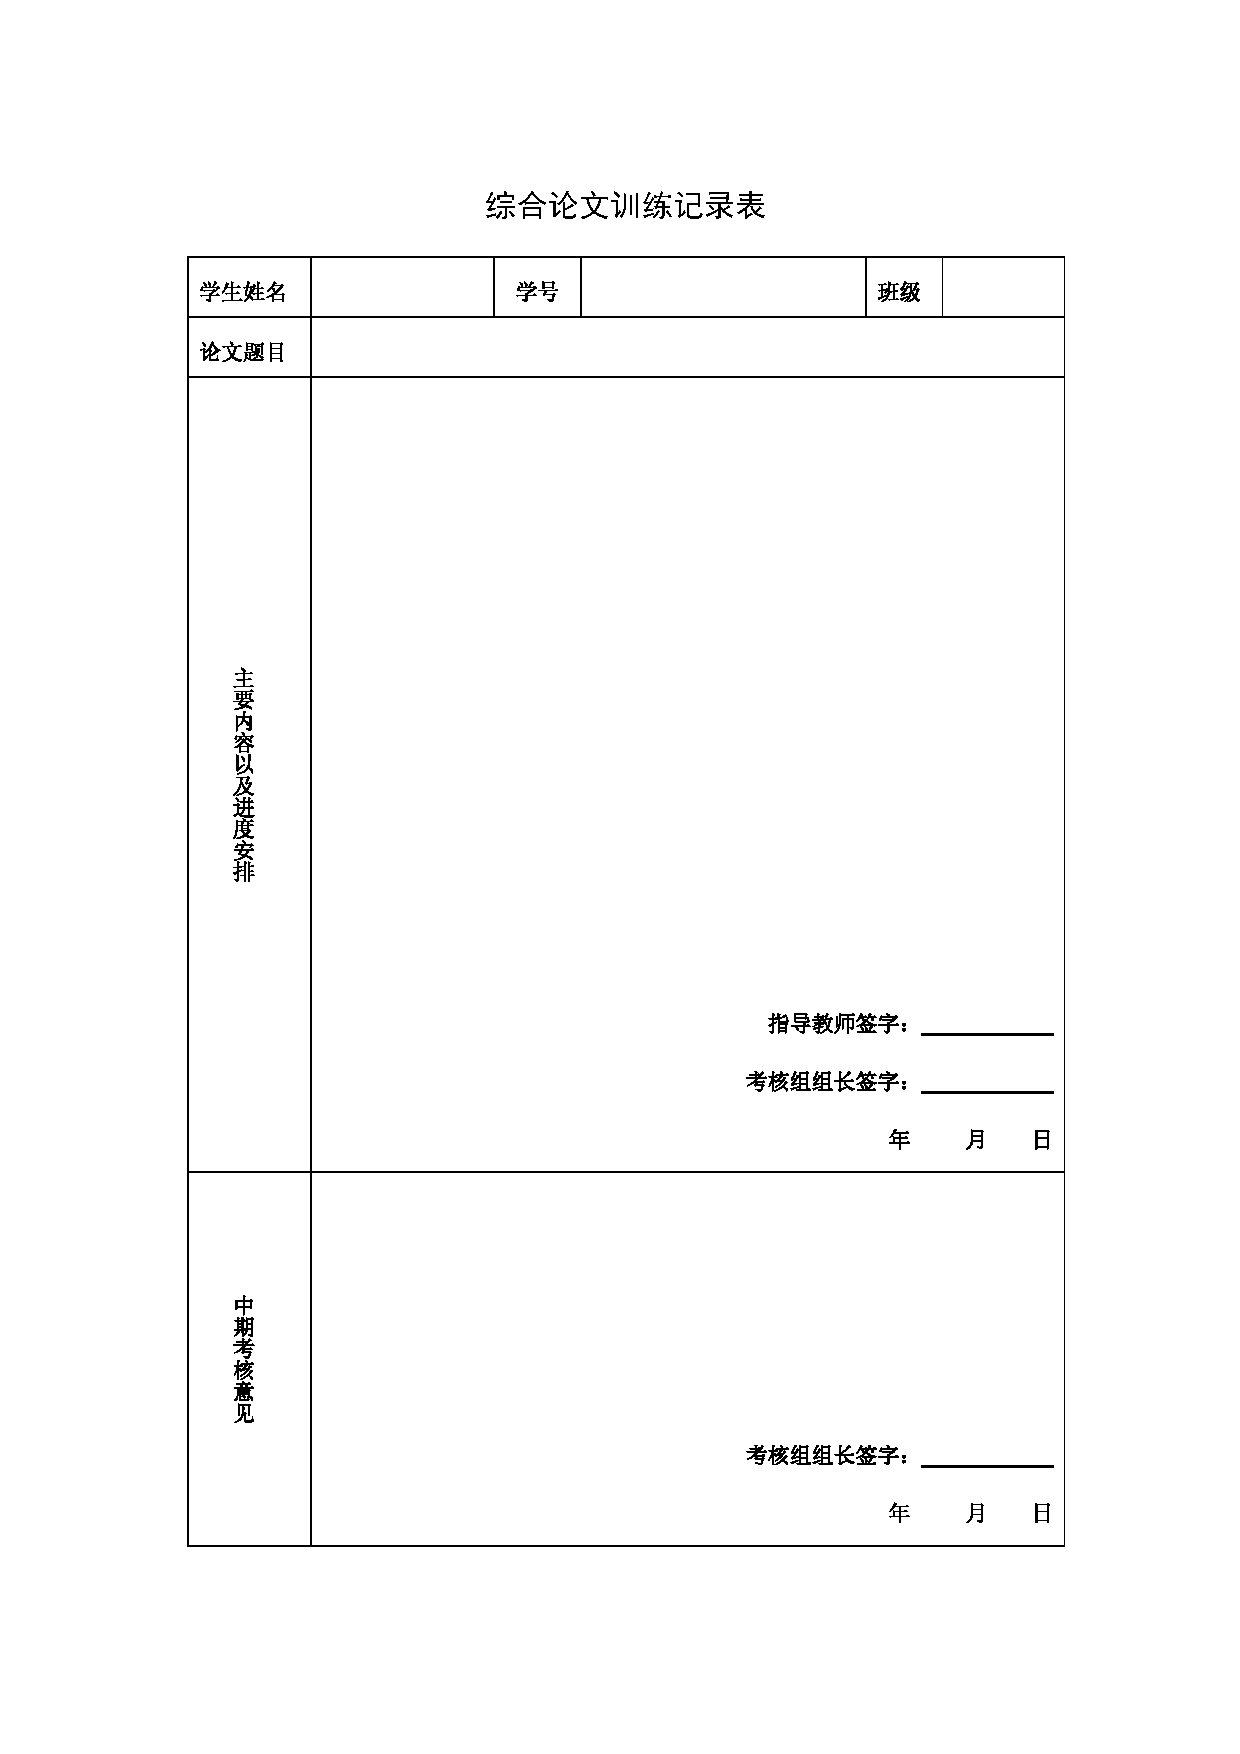
\includepdf[pages=-]{scan-record.pdf}
\end{document}
